%%%%%%%%%%%%%%%%%%%%%%%% editor.tex %%%%%%%%%%%%%%%%%%%%%%%%%%%%%
%
% sample root file for the contributions of a "contributed volume"
%
% Use this file as a template for your own input.
%
%%%%%%%%%%%%%%%%%%%%%%%%%%%%% Springer %%%%%%%%%%%%%%%%%%%%%%%%%%


% RECOMMENDED %%%%%%%%%%%%%%%%%%%%%%%%%%%%%%%%%%%%%%%%%%%%%%%%%%%
\documentclass[graybox, envcountchap]{styles/svmult}

% general metadata:
\author{soulmachine@gmail.com}
\title{Machine Learning Cheat Sheet}
\subtitle{Classical equations, diagrams and tricks in machine learning}

% choose options for [] as required from the list
% in the Reference Guide

\usepackage{amssymb,amsmath,bm}
\DeclareMathAlphabet{\mathcal}{OMS}{cmsy}{m}{n}
\usepackage{textcomp}
\newcommand\abs[1]{\left\lvert#1\right\rvert}
\usepackage{longtable}
\usepackage{algorithm2e}
\usepackage{tocbibind}
\renewcommand{\bibname}{References}
\usepackage{mathptmx}        % selects Times Roman as basic font
\usepackage{helvet}          % selects Helvetica as sans-serif font
\usepackage{courier}         % selects Courier as typewriter font
%\usepackage{type1cm}        % activate if the above 3 fonts are 
                             % not available on your system

\usepackage{makeidx}         % allows index generation
\usepackage{graphicx}        % standard LaTeX graphics tool
                             % when including figure files
\usepackage[justification=centering]{caption}
\usepackage{multicol}        % used for the two-column index
\usepackage[bottom]{footmisc}% places footnotes at page bottom
\usepackage[bookmarksnumbered=true,
            bookmarksopen=true,
            colorlinks=true,
            linkcolor=blue,
            anchorcolor=blue,
            citecolor=blue
           ]{hyperref}

\graphicspath{{figures/}}

% see the list of further useful packages in the Reference Guide

\makeindex             % used for the subject index
                       % please use the style svind.ist with
                       % your makeindex program

%%%%%%%%%%%%%%%%%%%%%%%%%%%%%%%%%%%%%%%%%%%%%%%%%%%%%%%%%%%%%%%%%

\begin{document}

\frontmatter%%%%%%%%%%%%%%%%%%%%%%%%%%%%%%%%%%%%%%%%%%%%%%%%%%%%%%

\begin{titlepage}

\url{https://github.com/soulmachine/machine-learning-cheat-sheet}

\end{titlepage}

\newpage

\noindent \textcopyright  2013 soulmachine \\
Except where otherwise noted, This document is licensed under a Creative Commons 
Attribution-ShareAlike 3.0 Unported (CC BY-SA3.0) license \\ (\url{http://creativecommons.org/licenses/by/3.0/}).

%%%%%%%%%%%%%%%%%%%%%%%% dedic.tex %%%%%%%%%%%%%%%%%%%%%%%%%%
%
% sample dedication
%
% Use this file as a template for your own input.
%
%%%%%%%%%%%%%%%%%%%%%%%% Springer %%%%%%%%%%%%%%%%%%%%%%%%%%

\begin{dedication}
This book is dedicated to my girl friend Jie Liu, thanks for her companion.
\end{dedication}




%%%%%%%%%%%%%%%%%%%%%%%foreword.tex%%%%%%%%%%%%%%%%%%%%%%%%%%%
% sample foreword
%
% Use this file as a template for your own input.
%
%%%%%%%%%%%%%%%%%%%%%%%% Springer %%%%%%%%%%%%%%%%%%%%%%%%%%

\foreword

Use the template \textit{foreword.tex} together with the Springer document class SVMono (monograph-type books) or SVMult (edited books) to style your foreword\index{foreword} in the Springer layout. 

The foreword covers introductory remarks preceding the text of a book that are written by a \textit{person other than the author or editor} of the book. If applicable, the foreword precedes the preface which is written by the author or editor of the book.


\vspace{\baselineskip}
\begin{flushright}\noindent
Place, month year\hfill {\it Firstname  Surname}\\
\end{flushright}



%%%%%%%%%%%%%%%%%%%%%%preface.tex%%%%%%%%%%%%%%%%%%%%%%%%%%%%%%%%%%%%%%%%%
% sample preface
%
% Use this file as a template for your own input.
%
%%%%%%%%%%%%%%%%%%%%%%%% Springer %%%%%%%%%%%%%%%%%%%%%%%%%%

\preface

This cheat sheet contains many classical equations and diagrams on machine learning, which will help you quickly recall knowledge and ideas in machine learning.

This cheat sheet has three significant advantages:
\begin{enumerate}
\item Strong typed. Compared to programming languages, mathematical formulas are weekly typed. For example, $X$ can be a set, a random variable, or a matrix. This causes difficulty in understanding the meaning of formulas. In this cheat sheet, I try my best to standardize symbols used, see section \S \ref{sec:Notation}.
\item More parentheses. In machine leaning, authors are prone to omit parentheses, brackets and braces,  this usually causes ambiguity in mathematical formulas. In this cheat sheet, I use parentheses(brackets and braces) at where they are needed, to make formulas easy to understand.
\item Less thinking jumps. In many books, authors are prone to omit some steps that are trivial in his option. But it often makes readers get lost in the middle way of derivation.
\end{enumerate}

\vspace{\baselineskip}
\begin{flushright}\noindent
At Tsinghua University, May 2013\hfill {\it soulmachine} \\
\end{flushright}



%%%%%%%%%%%%%%%%%%%%%%%acknow.tex%%%%%%%%%%%%%%%%%%%%%%%%%%%%%%%%%%%%%%%%%
% sample acknowledgement chapter
%
% Use this file as a template for your own input.
%
%%%%%%%%%%%%%%%%%%%%%%%% Springer %%%%%%%%%%%%%%%%%%%%%%%%%%

\extrachap{Acknowledgements}

Use the template \emph{acknow.tex} together with the Springer document class SVMono (monograph-type books) or SVMult (edited books) if you prefer to set your acknowledgement section as a separate chapter instead of including it as last part of your preface.



\tableofcontents
%%%%%%%%%%%%%%%%%%%%clist.tex %%%%%%%%%%%%%%%%%%%%%%%%
%                                                    
% sample list of contributors and their addresses    
%                                                    
% Use this file as a template for your own input.    
%                                                    
%%%%%%%%%%%%%%%%%%%%%%%% Springer %%%%%%%%%%%%%%%%%%%%
\contributors

\begin{thecontriblist}
Wei Zhang
\at PhD candidate at the Institute of Software, Chinese Academy of Sciences (ISCAS), Beijing, P.R.CHINA, \email{zh3feng@gmail.com}, has written chapters of Naive Bayes and SVM.
\and
Fei Pan
\at Master at Beijing University of Technology, Beijing, P.R.CHINA, \email{example@gmail.com}, has written chapters of KMeans, AdaBoost.
\and
Yong Li
\at PhD candidate at the Institute of Automation of the Chinese Academy of Sciences (CASIA), Beijing, P.R.CHINA, \email{liyong3forever@gmail.com}, has written chapters of Logistic Regression.
\and
Jiankou Li
\at PhD candidate at the Institute of Software, Chinese Academy of Sciences (ISCAS), Beijing, P.R.CHINA, \email{lijiankoucoco@163.com}, has written chapters of BayesNet.
\end{thecontriblist}
%%%%%%%%%%%%%%%%%%%%%%%acronym.tex%%%%%%%%%%%%%%%%%%%%%%%%%%%%%%%%%%%%%%%%%
% sample list of acronyms
%
% Use this file as a template for your own input.
%
%%%%%%%%%%%%%%%%%%%%%%%% Springer %%%%%%%%%%%%%%%%%%%%%%%%%%

\extrachap{Acronyms}

Use the template \emph{acronym.tex} together with the Springer document class SVMono (monograph-type books) or SVMult (edited books) to style your list(s) of abbreviations or symbols in the Springer layout.

Lists of abbreviations\index{acronyms, list of}, symbols\index{symbols, list of} and the like are easily formatted with the help of the Springer-enhanced \verb|description| environment.

\begin{description}[CABR]
\item[ABC]{Spelled-out abbreviation and definition}
\item[BABI]{Spelled-out abbreviation and definition}
\item[CABR]{Spelled-out abbreviation and definition}
\end{description}
\Extrachap{Notation}
\label{sec:Notation}

\section*{Introduction}
It is very difficult to come up with a single, consistent notation to cover the wide variety of
data, models and algorithms that we discuss. Furthermore, conventions difer between machine
learning and statistics, and between different books and papers. Nevertheless, we have tried
to be as consistent as possible. Below we summarize most of the notation used in this book,
although individual sections may introduce new notation. Note also that the same symbol may
have different meanings depending on the context, although we try to avoid this where possible.


\section*{General math notation}

\begin{longtable}{ll}
\hline\noalign{\smallskip}
\textbf{Symbol} & \textbf{Meaning} \\
\noalign{\smallskip}\hline\noalign{\smallskip}
$\lfloor x \rfloor$ & Floor of $x$, i.e., round down to nearest integer\\
$\lceil x \rceil$ & Ceiling of $x$, i.e., round down to nearest integer\\
$\vec{x} \otimes \vec{y}$ & Convolution of $\vec{x}$ and $\vec{y}$\\
$\vec{x} \odot \vec{y}$ & Hadamard (elementwise) product of $\vec{x}$ and $\vec{y}$\\
$a \wedge b$ & logical AND\\
$a \vee b$ & logical OR\\
$\neg a$ & logical NOT\\
$\mathbb{I}(x)$ & Indicator function, $\mathbb{I}(x)=1$ if x is true, else $\mathbb{I}(x)=0$\\
$\infty$ & Infinity\\
$\rightarrow$ & Tends towards, e.g., $n \rightarrow \infty$\\
$\propto$ &Proportional to, so $y = ax$ can be written as $y \propto x$\\
$\abs{x}$ & Absolute value\\
$\abs{\mathcal{S}}$ & Size (cardinality) of a set\\
$n!$ & Factorial function\\
$\nabla$ & Vector of first derivatives\\
$\nabla^2$ & Hessian matrix of second derivatives\\
$\triangleq$ & Defined as\\
$O(\cdot)$ & Big-O: roughly means order of magnitude\\
$\mathbb{R}$ & The real numbers\\
$1:n$ & Range (Matlab convention): $1:n = {1, 2,...,n}$\\
$\approx$ & Approximately equal to\\
$\arg\max\limits_x f(x)$ & Argmax: the value $x$ that maximizes $f$\\
$B(a,b)$ & Beta function, $B(a,b)=\dfrac{\Gamma(a)\Gamma(b)}{\Gamma(a+b)}$\\
$B(\vec{\alpha})$ & Multivariate beta function, $\dfrac{\prod\limits_k \Gamma(\alpha_k)}{\Gamma(\sum\limits_k \alpha_k)}$\\
$\binom{n}{k}$ & $n$ choose $k$ , equal to $n!/(k!(n−k )!)$\\
$\delta(x)$ & Dirac delta function,$\delta(x)=\infty$ if $x=0$, else $\delta(x)=0$\\
$exp(x)$ & Exponential function $e^x$\\
$\Gamma(x)$ & Gamma function, $\Gamma(x)=\int_0^\infty u^{x-1}e^{-u}\mathrm{d}u$\\
$\Psi(x)$ &  Digamma function,$Psi(x)=\dfrac{d}{dx}\log\Gamma(x)$\\
$\mathcal{X}$ & A set from which values are drawn (e.g.,$\mathcal{X}=\mathbb{R}^D$)\\
\noalign{\smallskip}\hline\noalign{\smallskip}
\end{longtable}


\section*{Linear algebra notation}
We use boldface lower-case to denote vectors, such as $\vec{x}$, and boldface upper-case to denote matrices, such as $\vec{X}$. We denote entries in a matrix by non-bold upper case letters, such as $X_{ij}$. 

Vectors are assumed to be column vectors, unless noted otherwise. We use $(x_1,\cdots,x_D)$ to denote a column vector created by stacking $D$ scalars. If we write $\vec{X}=(\vec{x}_1,\cdots,\vec{x}_n)$, where the left hand side is a matrix, we mean to stack the $\vec{x}_i$ along the columns, creating a matrix. 

\begin{longtable}{ll}
\hline\noalign{\smallskip}
\textbf{Symbol} & \textbf{Meaning} \\
\noalign{\smallskip}\hline\noalign{\smallskip}
$\vec{X} \succ 0$ & $\vec{X}$ is a positive definite matrix\\
$tr(\vec{X})$ & Trace of a matrix\\
$det(\vec{X})$ & Determinant of matrix $\vec{X}$\\
$\abs{\vec{X}}$ & Determinant of matrix $\vec{X}$\\
$\vec{X}^{-1}$ & Inverse of a matrix\\
$\vec{X}^{\dagger}$ & Pseudo-inverse of a matrix\\
$\vec{X}^T$ & Transpose of a matrix\\
$\vec{x}^T$ & Transpose of a vector\\
$diag(x)$ & Diagonal matrix made from vector $\vec{x}$\\
$diag(X)$ & Diagonal vector extracted from matrix $\vec{X}$\\
$\vec{I}$ or $\vec{I}_d$ & Identity matrix of size $d \times d$ (ones on diagonal, zeros of)\\
$\vec{1}$ or $\vec{1}_d$ & Vector of ones (of length $d$)\\
$\vec{0}$ or $\vec{0}_d$ & Vector of zeros (of length $d$)\\
$\abs{\abs{\vec{x}}}=\abs{\abs{\vec{x}}}_2$ & Euclidean or $\ell_2$ norm $\sqrt{\sum\limits_{j=1}^{d} x_j^2}$\\
$\abs{\abs{\vec{x}}}_1$ & $\ell_1$ norm $\sum\limits_{j=1}^{d} \abs{x_j}$\\
$\vec{X}_{:,j}$ & j'th column of matrix\\
$\vec{X}_{i,:}$ & transpose of $i$'th row of matrix (a column vector)\\
$\vec{X}_{i,j}$ & Element $(i,j)$ of matrix $\vec{X}$ \\
$\vec{x} \otimes \vec{y}$ & Tensor product of $\vec{x}$ and $\vec{y}$\\
\noalign{\smallskip}\hline\noalign{\smallskip}
\end{longtable}


\section*{Probability notation}
We denote random and fixed scalars by lower case, random and fixed vectors by bold lower case, and random and fixed matrices by bold upper case. Occasionally we use non-bold upper case to denote scalar random variables. Also, we use $p()$ for both discrete and continuous random variables

\begin{longtable}{ll}
\hline\noalign{\smallskip}
\textbf{Symbol} & \textbf{Meaning} \\
\noalign{\smallskip}\hline\noalign{\smallskip}
$X,Y$ & Random variable\\
$P()$ & Probability of a random event\\
$F()$ & Cumulative distribution function(CDF), also called distribution function\\
$p(x)$ & Probability mass function(PMF)\\
$f(x)$ & probability density function(PDF) \\
$F(x,y)$ & Joint CDF\\
$p(x,y)$ & Joint PMF \\
$f(x,y)$ & Joint PDF\\
$p(X|Y)$ & Conditional PMF, also called conditional probability\\
$f_{X|Y}(x|y)$ & Conditional PDF\\
$X \perp Y$ & X is independent of Y\\
$X \not\perp Y$ & X is not independent of Y\\
$X \perp Y | Z $ & X is conditionally independent of Y given Z\\
$X \not\perp Y | Z $ & X is not conditionally independent of Y given Z\\
$X \sim p$ & X is distributed according to distribution $p$\\
$\vec{\alpha}$ & Parameters of a Beta or Dirichlet distribution\\
$\mathrn{cov}[X]$ & Covariance of X\\
$\mathbb{E}[X]$ & Expected value of X\\
$\mathbb{E}_q[X]$ & Expected value of X wrt distribution $q$\\
$\mathbb{H}(X)$ or $\mathbb{H}(p)$ & Entropy of distribution $p(X)$\\
$\mathbb{I}(X;Y)$ & Mutual information between X and Y\\
$\mathbb{KL}(p||q)$ & KL divergence from distribution $p$ to $q$\\
$\ell(\vec{\theta})$ & Log-likelihood function\\
$L(\theta,a)$ & Loss function for taking action $a$ when true state of nature is $\theta$\\
$\lambda$ & Precision (inverse variance) $\lambda=1/\sigma^2$\\
$\Lambda$ & Precision matrix $\Lambda=\Sigma^{-1}$\\
mode$[\vec X]$ & Most probable value of $\vec X$\\
$\mu$ & Mean of a scalar distribution\\
$\vec{\mu}$ & Mean of a multivariate distribution\\
$\Phi$ & cdf of standard normal\\
$\phi$ & pdf of standard normal\\
$\vec{\pi}$ & multinomial parameter vector, Stationary distribution of Markov chain\\
$\rho$ & Correlation coefficient \\
sigm($x$) & Sigmoid (logistic) function,$\dfrac{1}{1+e^{-x}}$\\
$\sigma^2$ & Variance\\
$\Sigma$ & Covariance matrix\\
var[$x$] & Variance of $x$\\
$\nu$ & Degrees of freedom parameter\\
Z & Normalization constant of a probability distribution\\
\noalign{\smallskip}\hline\noalign{\smallskip}
\end{longtable}

\section*{Machine learning/statistics notation}
In general, we use upper case letters to denote constants, such as $C, K, M, N, T$, etc. We use lower case letters as dummy indexes of the appropriate range, such as $c=1:C$ to index classes, $i=1:M$ to index data cases, $j=1:N$ to index input features, $k=1:K$ to index states or clusters, $t=1:T$ to index time, etc.

We use $x$ to represent an observed data vector. In a supervised problem, we use $y$ or $\vec{y}$ to represent the desired output label. We use $\vec{z}$ to represent a hidden variable. Sometimes we also use $q$ to represent a hidden discrete variable.

\begin{longtable}{ll}
\hline\noalign{\smallskip}
\textbf{Symbol} & \textbf{Meaning} \\
\noalign{\smallskip}\hline\noalign{\smallskip}
$C$ & Number of classes\\
$D$ & Dimensionality of data vector (number of features)\\
$N$ & Number of data cases\\
$N_c$ & Number of examples of class $c$,$N_c=\sum_{i=1}^{N}\mathbb{I}(y_i=c)$\\
$R$ & Number of outputs (response variables)\\
$\mathcal{D}$ & Training data $\mathcal{D}=\left\{(\vec{x}_i,y_i) | i=1:N\right\}$\\
$\mathcal{D}_{test}$ & Test data\\
$\mathcal{X}$ & Input space\\
$\mathcal{Y}$ & Output space\\
$K$ & Number of states or dimensions of a variable (often latent)\\
$k(x,y)$ & Kernel function\\
$\vec{K}$ & Kernel matrix\\
$\mathcal{H}$ & Hypothesis space\\
$L$ & Loss function \\
$J(\vec{\theta})$ & Cost function\\
$f(\vec{x})$ & Decision function\\
$P(y|\vec{x})$ & TODO\\
$\lambda$ & Strength of $\ell_2$ or $\ell_1 regularizer$\\
$\phi(x)$ & Basis function expansion of feature vector $\vec{x}$\\
$\Phi$ & Basis function expansion of design matrix $\vec{X}$\\
$q()$ & Approximate or proposal distribution\\
$Q(\vec{\theta},\vec{\theta}_{old})$ & Auxiliary function in EM\\
$T$ & Length of a sequence\\
$T(\mathcal{D})$ & Test statistic for data\\
$\vec{T}$ & Transition matrix of Markov chain\\
$\vec{\theta}$ & Parameter vector\\
$\vec{\theta}^{(s)}$ & $s$'th sample of parameter vector\\
$\hat{\vec{\theta}}$ & Estimate (usually MLE or MAP) of $\vec{\theta}$\\
$\hat{\vec{\theta}}_{MLE}$ & Maximum likelihood estimate of $\vec{\theta}$\\
$\hat{\vec{\theta}}_{MAP}$ & MAP estimate of $\vec{\theta}$\\
$\bar{\vec{\theta}}$ & Estimate (usually posterior mean) of  $\vec{\theta}$\\
$\vec{w}$ & Vector of regression weights (called $\vec{\beta}$ in statistics)\\
b & intercept (called $\varepsilon$ in statistics)\\
$\vec{W}$ & Matrix of regression weights\\
$x_{ij}$ & Component (i.e., feature) $j$ of data case $i$ ,for $i=1:N ,j=1:D$\\
$\vec{x}_i$ & Training case, $i=1:N$\\
$\vec{X}$ & Design matrix of size $N \times D$\\
$\bar{\vec{x}}$ & Empirical mean $\bar{\vec{x}}=\dfrac{1}{N}\sum_{i=1}^{N} \vec{x}_i$\\
$\tilde{\vec{x}}$ & Future test case\\
$\vec{x}_*$ & Feature test case\\
$\vec{y}$ & Vector of all training labels $\vec{y} =(y_1,...,y_N)$\\
$z_{ij}$ & Latent component $j$ for case $i$\\
\noalign{\smallskip}\hline\noalign{\smallskip}
\end{longtable}

\twocolumn


\mainmatter%%%%%%%%%%%%%%%%%%%%%%%%%%%%%%%%%%%%%%%%%%%%%%%%%%%%%%%
%%%%%%%%%%%%%%%%%%%%%%part.tex%%%%%%%%%%%%%%%%%%%%%%%%%%%%%%%%%%
% 
% sample part title
%
% Use this file as a template for your own input.
%
%%%%%%%%%%%%%%%%%%%%%%%% Springer %%%%%%%%%%%%%%%%%%%%%%%%%%

\begin{partbacktext}
\part{Part Title}
\noindent Use the template \emph{part.tex} together with the Springer document class SVMono (monograph-type books) or SVMult (edited books) to style your part title page and, if desired, a short introductory text (maximum one page) on its verso page in the Springer layout.

\end{partbacktext}
\chapter{Introduction}

\section{Types of machine learning}
\begin{equation}\nonumber
\text{Machine learning}\begin{cases}
\text{Supervised learning} \begin{cases} \text{Classfication} \\ \text{Regression} \end{cases}\\
\text{Unsupervised learning} \begin{cases} \text{Discovering clusters} \\ \text{Discovering latent factors} \\ \text{Discovering graph structure} \\ \text{Matrix completion} \end{cases}\\
\end{cases}
\end{equation}


\section{Three elements of a machine learning model}

\textbf{Model = Representation + Evaluation + Optimization}\footnote{Domingos, P. A few useful things to know about machine learning. Commun. ACM. 55(10):78–87 (2012).}


\subsection{Representation}
In supervised learning, a model must be represented as a conditional probability distribution $P(y|\vec{x})$(usually we call it classifier) or a decision function $f(x)$. The set of classifiers(or decision functions) is called the hypothesis space of the model. Choosing a representation for a model is tantamount to choosing the hypothesis space that it can possibly learn. 


\subsection{Evaluation}
In the hypothesis space, an evaluation function (also called objective function or risk function) is needed to distinguish good classifiers(or decision functions) from bad ones.


\subsubsection{Loss function and risk function}
\label{sec:Loss-function-and-risk-function}

\begin{definition}
In order to measure how well a function fits the training data, a \textbf{loss function} $L:Y \times Y \rightarrow R \geq 0$ is defined. For training example $(x_i,y_i)$, the loss of predicting the value $\widehat{y}$ is $L(y_i,\widehat{y})$.
\end{definition}

The following is some common loss functions:
\begin{enumerate}
\item 0-1 loss function $L(Y,f(X))=I(Y,f(X))=\begin{cases} 1, & Y=f(X) \\ 0, & Y \neq f(X) \end{cases}$
\item Quadratic loss function $L(Y,f(X))=\left(Y-f(X)\right)^2$
\item Absolute loss function $L(Y,f(X))=\abs{Y-f(X)}$
\item Logarithmic loss function $L(Y,P(Y|X))=-\log{P(Y|X)}$
\end{enumerate}

\begin{definition}
The risk of function $f$ is defined as the expected loss of $f$:
\begin{equation}\label{eqn:expected-loss}
R_{exp}(f)=E_p\left[L\left(Y,f(X)\right)\right]=\int _{X \times Y} L\left(y,f(x)\right)P(x,y)\mathrm{d}x\mathrm{d}y
\end{equation}
which is also called expected loss or \textbf{risk function}.
\end{definition}

\begin{definition}
The risk function $R_{exp}(f)$ can be estimated from the training data as
\begin{equation}
R_{emp}(f)=\dfrac{1}{N}\sum\limits_{i=1}^{N} L\left(y_i,f(x_i)\right)
\end{equation}
which is also called empirical loss or \textbf{empirical risk}.
\end{definition}

You can define your own loss function, but if you're a novice, you're probably better off using one from the literature. There are conditions that loss functions should meet\footnote{\url{http://t.cn/zTrDxLO}}:
\begin{enumerate}
\item They should approximate the actual loss you're trying to minimize. As was said in the other answer, the standard loss functions for classification is zero-one-loss (misclassification rate) and the ones used for training classifiers are approximations of that loss.
\item The loss function should work with your intended optimization algorithm. That's why zero-one-loss is not used directly: it doesn't work with gradient-based optimization methods since it doesn't have a well-defined gradient (or even a subgradient, like the hinge loss for SVMs has).

The main algorithm that optimizes the zero-one-loss directly is the old perceptron algorithm(chapter \S \ref{chap:Perceptron}).
\end{enumerate}


\subsubsection{ERM and SRM}
\begin{definition}
ERM(Empirical risk minimization)
\begin{equation}
\min\limits _{f \in \mathcal{F}} R_{emp}(f)=\min\limits _{f \in \mathcal{F}} \dfrac{1}{N}\sum\limits_{i=1}^{N} L\left(y_i,f(x_i)\right)
\end{equation}
\end{definition}

\begin{definition}
Structural risk
\begin{equation}
R_{smp}(f)=\dfrac{1}{N}\sum\limits_{i=1}^{N} L\left(y_i,f(x_i)\right) +\lambda J(f)
\end{equation}
\end{definition}

\begin{definition}
SRM(Structural risk minimization)
\begin{equation}
\min\limits _{f \in \mathcal{F}} R_{srm}(f)=\min\limits _{f \in \mathcal{F}} \dfrac{1}{N}\sum\limits_{i=1}^{N} L\left(y_i,f(x_i)\right) +\lambda J(f)
\end{equation}
\end{definition}


\subsection{Optimization}
Finally, we need a \textbf{training algorithm}(also called \textbf{learning algorithm}) to search among the classifiers in the the hypothesis space for the highest-scoring one. The choice of optimization technique is key to the \textbf{efficiency} of the model.


\section{Cross validation}
\label{sec:Cross-validation}
\begin{definition}
\textbf{Cross validation}, sometimes called \emph{rotation estimation}, is a \emph{model validation} technique for assessing how the results of a statistical analysis will generalize to an independent data set\footnote{\url{http://en.wikipedia.org/wiki/Cross-validation_(statistics)}}.
\end{definition}

Common types of cross-validation:
\begin{enumerate}
\item K-fold cross-validation. In k-fold cross-validation, the original sample is randomly partitioned into k equal size subsamples. Of the k subsamples, a single subsample is retained as the validation data for testing the model, and the remaining k − 1 subsamples are used as training data.
\item 2-fold cross-validation. Also, called simple cross-validation or holdout method. This is the simplest variation of k-fold cross-validation, k=2.
\item Leave-one-out cross-validation(\emph{LOOCV}). k=M, the number of original samples.
\end{enumerate}

\chapter{Probability}

\section{Frequentists vs. Bayesians}
what is probability? 

One is called the \textbf{frequentist} interpretation. In this view, probabilities represent long run frequencies of events. For example, the above statement means that, if we flip the coin many times, we expect it to land heads about half the time.

The other interpretation is called the \textbf{Bayesian} interpretation of probability. In this view, probability is used to quantify our \textbf{uncertainty} about something; hence it is fundamentally related to information rather than repeated trials (Jaynes 2003). In the Bayesian view, the above statement means we believe the coin is equally likely to land heads or tails on the next toss

One big advantage of the Bayesian interpretation is that it can be used to model our uncertainty about events that do not have long term frequencies. For example, we might want to compute the probability that the polar ice cap will melt by 2020 CE. This event will happen zero or one times, but cannot happen repeatedly. Nevertheless, we ought to be able to quantify our uncertainty about this event. To give another machine learning oriented example, we might have observed a “blip” on our radar screen, and want to compute the probability distribution over the location of the corresponding target (be it a bird, plane, or missile). In all these cases, the idea of repeated trials does not make sense, but the Bayesian interpretation is valid and indeed quite natural. We shall therefore adopt the Bayesian interpretation in this book. Fortunately, the basic rules of probability theory are the same, no matter which interpretation is adopted.


\section{A brief review of probability theory}


\subsection{Basic concepts}
We denote a random event by defining a \textbf{random variable} $X$.

\textbf{Descrete random variable}: $X$ can take on any value from a finite or countably infinite set.

\textbf{Continuous random variable}: the value of $X$ is real-valued.


\subsubsection{CDF}

\begin{equation}
F(x) \triangleq P(X \leq x)=\begin{cases}
\sum_{u \leq x}p(u) & \text{, discrete}\\
\int_{-\infty}^{x} f(u)\mathrm{d}u & \text{, continuous}\\
\end{cases}
\end{equation}


\subsubsection{PMF and PDF}
For descrete random variable, We denote the probability of the event that $X=x$ by $P(X=x)$, or just $p(x)$ for short. Here $p(x)$ is called a \textbf{probability mass function} or \textbf{PMF}.A probability mass function is a function that gives the probability that a discrete random variable is exactly equal to some value\footnote{\url{http://en.wikipedia.org/wiki/Probability_mass_function}}. This satisfies the properties $0 \leq p(x) \leq 1$ and $\sum_{x \in \mathcal{X}} p(x)=1$.

For continuous variable, in the equation $F(x)=\int_{-\infty}^{x} f(u)\mathrm{d}u$, the function $f(x)$ is called a \textbf{probability density function} or \textbf{PDF}. A probability density function is a function that describes the relative likelihood for this random variable to take on a given value\footnote{\url{http://en.wikipedia.org/wiki/Probability_density_function}}.This satisfies the properties $f(x) \geq 0$ and $\int_{-\infty}^{\infty} f(x)\mathrm{d}x=1$.


\subsection{Mutivariate random variables}


\subsubsection{Joint CDF}
We denote joint CDF by $F(x,y) \triangleq P(X \leq x \cap Y \leq y)=P(X \leq x , Y \leq y)$.

\begin{equation}
F(x,y) \triangleq P(X \leq x, Y \leq y)=\begin{cases}
\sum_{u \leq x, v \leq y}p(u,v) \\
\int_{-\infty}^{x}\int_{-\infty}^{y} f(u,v)\mathrm{d}u\mathrm{d}v \\
\end{cases}
\end{equation}

\textbf{product rule}:
\begin{equation}\label{eqn:product-rule}
p(X,Y)=P(X|Y)P(Y)
\end{equation}

\textbf{Chain rule}:
\begin{equation}
p(X_{1:N})=p(X_1)p(X_3|X_2,X_1)...p(X_N|X_{1:N-1})
\end{equation}


\subsubsection{Marginal distribution}
\textbf{Marginal CDF}:
\begin{equation}\begin{split}
& F_X(x) \triangleq F(x,+\infty)= \\
& \begin{cases}
\sum\limits_{x_i \leq x}P(X=x_i)=\sum\limits_{x_i \leq x}\sum\limits_{j=1}^{+\infty}P(X=x_i,Y=y_j) \\
\int_{-\infty}^{x}f_X(u)du=\int_{-\infty}^{x}\int_{-\infty}^{+\infty} f(u,v)\mathrm{d}u\mathrm{d}v \\
\end{cases}
\end{split}\end{equation}

\begin{equation}\begin{split}
& F_Y(y) \triangleq F(+\infty,y)= \\
& \begin{cases}
\sum\limits_{y_j \leq y}p(Y=y_j)=\sum\limits_{i=1}^{+\infty}\sum_{y_j \leq y}P(X=x_i,Y=y_j) \\
\int_{-\infty}^{y}f_Y(v)dv=\int_{-\infty}^{+\infty}\int_{-\infty}^{y} f(u,v)\mathrm{d}u\mathrm{d}v \\
\end{cases}
\end{split}\end{equation}

\textbf{Marginal PMF and PDF}:
\begin{equation} \begin{cases}
P(X=x_i)=\sum_{j=1}^{+\infty}P(X=x_i,Y=y_j) & \text{, descrete}\\
f_X(x)=\int_{-\infty}^{+\infty} f(x,y)\mathrm{d}y & \text{, continuous}\\
\end{cases}\end{equation}

\begin{equation}\begin{cases}
p(Y=y_j)=\sum_{i=1}^{+\infty}P(X=x_i,Y=y_j) & \text{, descrete}\\
f_Y(y)=\int_{-\infty}^{+\infty} f(x,y)\mathrm{d}x & \text{, continuous}\\
\end{cases}\end{equation}


\subsubsection{Conditional distribution}
\textbf{Conditional PMF}:
\begin{equation}
p(X=x_i|Y=y_j)=\dfrac{p(X=x_i,Y=y_j)}{p(Y=y_j)} \text{ if } p(Y)>0
\end{equation}
The pmf $p(X|Y)$ is called \textbf{conditional probability}.

\textbf{Conditional PDF}:
\begin{equation}
f_{X|Y}(x|y)=\dfrac{f(x,y)}{f_Y(y)}
\end{equation}

\subsection{Bayes rule}
\begin{equation}
\begin{split}
p(Y=y|X=x) & =\dfrac{p(X=x,Y=y)}{p(X=x)} \\
           & =\dfrac{p(X=x|Y=y)p(Y=y)}{\sum_{y'}p(X=x|Y=y')p(Y=y')}
\end{split}
\end{equation}


\subsection{Independence and conditional independence}
We say $X$ and $Y$ are unconditionally independent or marginally independent, denoted $X \perp Y$, if we can represent the joint as the product of the two marginals, i.e.,
\begin{equation}
X \perp Y=P(X,Y)=P(X)P(Y)
\end{equation}

We say $X$ and $Y$ are conditionally independent(CI) given $Z$ if the conditional joint can be written as a product of conditional marginals:
\begin{equation}
X \perp Y|Z=P(X,Y|Z)=P(X|Z)P(Y|Z)
\end{equation}

\subsection{Quantiles}
Since the cdf $F$ is a monotonically increasing function, it has an inverse; let us denote this by $F^{-1}$. If $F$ is the cdf of $X$ , then $F^{-1}(\alpha)$ is the value of $x_{\alpha}$ such that $P(X \leq x_{\alpha})=\alpha$; this is called the $\alpha$ quantile of $F$. The value $F^{-1}(0.5)$ is the \textbf{median} of the distribution, with half of the probability mass on the left, and half on the right. The values $F^{-1}(0.25)$ and $F^{−1}(0.75)$are the lower and upper \textbf{quartiles}.

\subsection{Mean and variance}
The most familiar property of a distribution is its \textbf{mean},or \textbf{expected value}, denoted by $\mu$. For discrete rv’s, it is defined as $\mathbb{E}[X] \triangleq \sum_{x \in \mathcal{X}}xp(x)$, and for continuous rv’s, it is defined as $\mathbb{E}[X] \triangleq \int_{\mathcal{X}}xp(x)\mathrm{d}x$. If this integral is not finite, the mean is not defined (we will see some examples of this later). 

The \textbf{variance} is a measure of the “spread” of a distribution, denoted by $\sigma^2$. This is defined as follows:
\begin{align}
var[X]& =\mathbb{E}[(X-\mu)^2] \\
      & =\int{(x-\mu)^2p(x)\mathrm{d}x} \nonumber \\
      & =\int{x^2p(x)\mathrm{d}x}+{\mu}^2\int{p(x)\mathrm{d}x}-2\mu\int{xp(x)\mathrm{d}x} \nonumber \\
	  & =\mathbb{E}[X^2]-{\mu}^2
\end{align}

from which we derive the useful result
\begin{equation}
\mathbb{E}[X^2]=\sigma^2+{\mu}^2
\end{equation}

The \textbf{standard deviation} is defined as
\begin{equation}
std[X] \triangleq \sqrt{var[X]}
\end{equation}

This is useful since it has the same units as $X$ itself.

\section{Some common discrete distributions}
In this section, we review some commonly used parametric distributions defined on discrete state spaces, both finite and countably infinite.


\subsection{The Bernoulli and binomial distributions}

\begin{definition}
Now suppose we toss a coin only once. Let $X \in \{0,1\}$ be a binary random variable, with probability of “success” or “heads” of $\theta$. We say that $X$ has a \textbf{Bernoulli distribution}. This is written as $X \sim \text{Ber}(\theta)$, where the pmf is defined as 
\begin{equation}
\text{Ber}(x|\theta) \triangleq \theta^{\mathbb{I}(x=1)}(1-\theta)^{\mathbb{I}(x=0)}
\end{equation}
\end{definition}


\begin{definition}
Suppose we toss a coin $n$ times. Let $X \in \{0,1,\cdots,n\}$ be the number of heads. If the probability of heads is $\theta$, then we say $X$ has a \textbf{binomial distribution}, written as $X \sim \text{Bin}(n, \theta)$. The pmf is given by 
\begin{equation}\label{eqn:binomial-pmf}
\text{Bin}(k|n,\theta) \triangleq \dbinom{n}{k}\theta^k(1-\theta)^{n-k}
\end{equation}
\end{definition}


\subsection{The multinoulli and multinomial distributions}

\begin{definition}
The Bernoulli distribution can be used to model the outcome of one coin tosses. To model the outcome of tossing a K-sided dice, let $\vec{x} =(\mathbb{I}(x=1),\cdots,\mathbb{I}(x=K)) \in \{0,1\}^K$ be a random vector(this is called \textbf{dummy encoding} or \textbf{one-hot encoding}), then we say $X$ has a \textbf{multinoulli distribution}(or \textbf{categorical distribution}), written as $X \sim \text{Cat}(\theta)$. The pmf is given by: 
\begin{equation}
p(\vec{x}) \triangleq \prod\limits_{k=1}^K\theta_k^{\mathbb{I}(x_k=1)}
\end{equation}
\end{definition}

\begin{definition}
Suppose we toss a K-sided dice $n$ times. Let $\vec{x} =(x_1,x_2,\cdots,x_K) \in \{0,1,\cdots,n\}^K$ be a random vector, where $x_j$ is the number of times side $j$ of the dice occurs, then we say $X$ has a \textbf{multinomial distribution}, written as $X \sim \text{Mu}(n, \vec{\theta})$. The pmf is given by 
\begin{equation}\label{eqn:multinomial-pmf}
p(\vec{x}) \triangleq \dbinom{n}{x_1 \cdots x_k} \prod\limits_{k=1}^K\theta_k^{x_k}
\end{equation}
where $\dbinom{n}{x_1 \cdots x_k} \triangleq \dfrac{n!}{x_1!x_2! \cdots x_K!}$
\end{definition}

Bernoulli distribution is just a special case of a Binomial distribution with $n=1$, and so is multinoulli distribution as to multinomial distribution. See Table \ref{tab:multinomial-summary} for a summary.

\begin{table}
\caption{Summary of the multinomial and related distributions.}
\label{tab:multinomial-summary}
\centering
\begin{tabular}{llll}
\hline\noalign{\smallskip}
Name & K & n & X \\
\noalign{\smallskip}\svhline\noalign{\smallskip}
Bernoulli & 1 & 1 & $x \in \{0,1\}$ \\
Binomial & 1 & - & $\vec{x} \in \{0,1,\cdots,n\}$ \\
Multinoulli & - & 1 & $\vec{x} \in \{0,1\}^K, \sum_{k=1}^K x_k=1$ \\
Multinomial & - & - & $\vec{x} \in \{0,1,\cdots,n\}^K, \sum_{k=1}^K x_k=n$ \\
\noalign{\smallskip}\hline
\end{tabular}
\end{table} 


\subsection{The Poisson distribution}
\begin{definition}
We say that $X \in \{0,1,2,\cdots\}$ has a \textbf{Poisson distribution} with parameter $\lambda>0$, written as $X \sim \text{Poi}(\lambda)$, if its pmf is
\begin{equation}
p(x|\lambda)=e^{-\lambda}\dfrac{\lambda^x}{x!}
\end{equation}
\end{definition}

The first term is just the normalization constant, required to ensure the distribution sums to 1.

The Poisson distribution is often used as a model for counts of rare events like radioactive decay and traffic accidents. 

\begin{table*}
\caption{Summary of Bernoulli, binomial multinoulli and multinomial distributions.}
\label{tab:Summary-distribution}
\centering
\begin{tabular}{llllll}
\hline\noalign{\smallskip}
Name & Written as & X & $p(x)$(or $p(\vec{x})$) & $\mathbb{E}[X]$ & $\text{var}[X]$ \\
\noalign{\smallskip}\svhline\noalign{\smallskip}
Bernoulli & $X \sim \text{Ber}(\theta)$ & $x \in \{0,1\}$ & $\theta^{\mathbb{I}(x=1)}(1-\theta)^{\mathbb{I}(x=0)}$ & $\theta$ & $\theta(1-\theta)$ \\
Binomial & $X \sim \text{Bin}(n,\theta)$ & $x \in \{0,1,\cdots,n\}$ & $\dbinom{n}{k}\theta^k(1-\theta)^{n-k}$ & $n\theta$ & $n\theta(1-\theta)$ \\
Multinoulli & $X \sim \text{Cat}(\vec{\theta})$ & $\vec{x} \in \{0,1\}^K, \sum_{k=1}^K x_k=1$ & $\prod\limits_{k=1}^K\theta_j^{\mathbb{I}(x_j=1)}$ & - & - \\
Multinomial & $X \sim \text{Mu}(n,\vec{\theta})$ & $\vec{x} \in \{0,1,\cdots,n\}^K, \sum_{k=1}^K x_k=n$ & $\dbinom{n}{x_1 \cdots x_k} \prod\limits_{k=1}^K\theta_j^{x_j}$ & - & - \\
Poisson & $X \sim \text{Poi}(\lambda)$ & $x \in \{0,1,2,\cdots\}$ & $e^{-\lambda}\dfrac{\lambda^x}{x!}$ & $\lambda$ & $\lambda$ \\
\noalign{\smallskip}\hline
\end{tabular}
\end{table*}


\subsection{The empirical distribution}
The \textbf{empirical distribution function}\footnote{\url{http://en.wikipedia.org/wiki/Empirical_distribution_function}}, or \textbf{empirical cdf}, is the cumulative distribution function associated with the empirical measure of the sample. Let $\mathcal{D}=\{x_1,x_2,\cdots,x_N\}$ be a sample set, it is defined as 
\begin{equation}
F_n(x) \triangleq \dfrac{1}{N}\sum\limits_{i=1}^N\mathbb{I}(x_i \leq x)
\end{equation}


\section{Some common continuous distributions}
In this section we present some commonly used univariate (one-dimensional) continuous probability distributions.


\subsection{Gaussian (normal) distribution}

% \begin{table}
% \caption{Summary of Gaussian distribution}
% \centering
% \begin{tabular}{cccccc}
% \hline\noalign{\smallskip}
% Name & Written as & $f(x)$ & $\mathbb{E}[X]$ & mode & $\text{var}[X]$ \\
% \noalign{\smallskip}\svhline\noalign{\smallskip}
% Gaussian distribution & $X \sim \mathcal{N}(\mu,\sigma^2)$ & $\dfrac{1}{\sqrt{2\pi}\sigma}e^{-\frac{1}{2\sigma^2}\left(x-\mu\right)^2}$ & $\mu$ & $\mu$ & $\sigma^2$ \\
% \noalign{\smallskip}\hline
% \end{tabular}
% \end{table} 

\begin{table}
\caption{Summary of Gaussian distribution.}
\centering
\begin{tabular}{cccccc}
\hline\noalign{\smallskip}
Written as & $f(x)$ & $\mathbb{E}[X]$ & mode & $\text{var}[X]$ \\
\noalign{\smallskip}\svhline\noalign{\smallskip}
$X \sim \mathcal{N}(\mu,\sigma^2)$ & $\dfrac{1}{\sqrt{2\pi}\sigma}e^{-\frac{1}{2\sigma^2}\left(x-\mu\right)^2}$ & $\mu$ & $\mu$ & $\sigma^2$ \\
\noalign{\smallskip}\hline
\end{tabular}
\end{table} 

If $X \sim N(0,1)$,we say $X$ follows a \textbf{standard normal} distribution.

The Gaussian distribution is the most widely used distribution in statistics. There are several reasons for this. 
\begin{enumerate}
\item First, it has two parameters which are easy to interpret, and which capture some of the most basic properties of a distribution, namely its mean and variance. 
\item Second,the central limit theorem (Section TODO) tells us that sums of independent random variables have an approximately Gaussian distribution, making it a good choice for modeling residual errors or “noise”. 
\item Third, the Gaussian distribution makes the least number of assumptions (has maximum entropy), subject to the constraint of having a specified mean and variance, as we show in Section TODO; this makes it a good default choice in many cases. 
\item Finally, it has a simple mathematical form, which results in easy to implement, but often highly effective, methods, as we will see. 
\end{enumerate}
See (Jaynes 2003, ch 7) for a more extensive discussion of why Gaussians are so widely used.


\subsection{Student's t-distribution}
\begin{table}
\caption{Summary of Student's t-distribution.}
\centering
\begin{tabular}{cccccc}
\hline\noalign{\smallskip}
Written as & $f(x)$ & $\mathbb{E}[X]$ & mode & $\text{var}[X]$ \\
\noalign{\smallskip}\svhline\noalign{\smallskip}
$X \sim \mathcal{T}(\mu,\sigma^2,\nu)$ & $\dfrac{\Gamma(\frac{\nu+1}{2})}{\sqrt{\nu\pi}\Gamma(\frac{\nu}{2})}\left[1+\dfrac{1}{\nu}\left(\dfrac{x-\mu}{\nu}\right)^2\right]$ & $\mu$ & $\mu$ & $\dfrac{\nu\sigma^2}{\nu-2}$ \\
\noalign{\smallskip}\hline
\end{tabular}
\end{table}
where  $\Gamma(x)$ is the gamma function:
\begin{equation}
\Gamma(x) \triangleq \int_0^\infty u^{x-1}e^{-u}\mathrm{d}x
\end{equation}
$\mu$ is the mean, $\sigma^2>0$ is the scale parameter, and $\nu>0$ is called the \textbf{degrees of freedom}. See Figure \ref{fig:pdfs-for-NTL} for some plots.

\begin{figure}[hbtp]
\centering
\subfloat[]{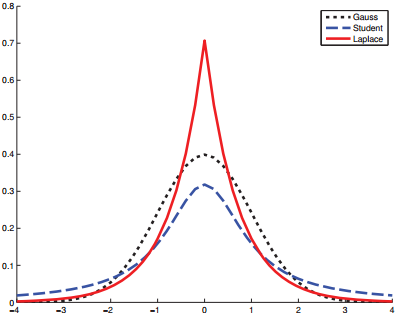
\includegraphics[scale=.70]{pdfs-for-NTL-a.png}} \\
\subfloat[]{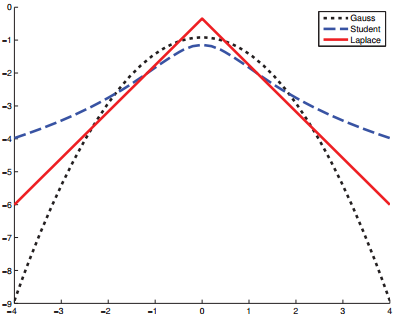
\includegraphics[scale=.70]{pdfs-for-NTL-b.png}}
\caption{(a) The pdf’s for a $\mathcal{N}(0,1)$, $\mathcal{T}(0,1,1)$ and $Lap(0,1/\sqrt{2})$. The mean is 0 and the variance is 1 for both the Gaussian and Laplace. The mean and variance of the Student is undefined when $\nu=1$.(b) Log of these pdf’s. Note that the Student distribution is not log-concave for any parameter value, unlike the Laplace distribution, which is always log-concave (and log-convex...) Nevertheless, both are unimodal.}
\label{fig:pdfs-for-NTL} 
\end{figure}

The variance is only defined if $\nu>2$. The mean is only defined if $\nu>1$.

As an illustration of the robustness of the Student distribution, consider Figure \ref{fig:robustness}. We see that the Gaussian is affected a lot, whereas the Student distribution hardly changes. This is because the Student has heavier tails, at least for small $\nu$(see Figure \ref{fig:pdfs-for-NTL}).

\begin{figure}[hbtp]
\centering
\subfloat[]{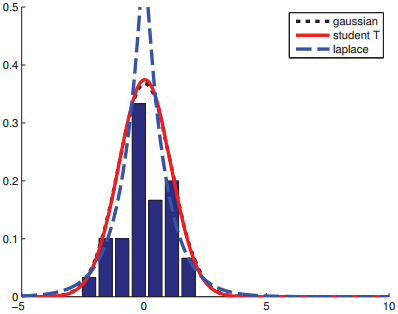
\includegraphics[scale=.70]{robustness-a.png}} \\
\subfloat[]{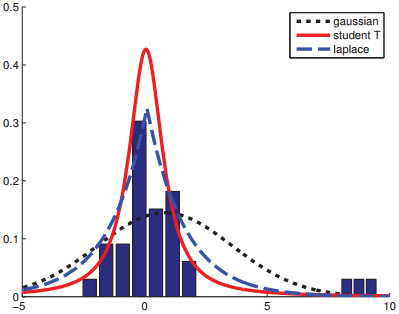
\includegraphics[scale=.70]{robustness-b.png}}
\caption{Illustration of the effect of outliers on fitting Gaussian, Student and Laplace distributions. (a) No outliers (the Gaussian and Student curves are on top of each other). (b) With outliers. We see that the Gaussian is more affected by outliers than the Student and Laplace distributions.}
\label{fig:robustness} 
\end{figure}

If $\nu=1$, this distribution is known as the \textbf{Cauchy} or \textbf{Lorentz} distribution. This is notable for having such heavy tails that the integral that defines the mean does not converge.

To ensure finite variance, we require $\nu>2$. It is common to use $\nu=4$, which gives good performance in a range of problems (Lange et al. 1989). For $\nu \gg 5$, the Student distribution rapidly approaches a Gaussian distribution and loses its robustness properties.


\subsection{The Laplace distribution}
\begin{table}
\caption{Summary of Laplace distribution.}
\centering
\begin{tabular}{cccccc}
\hline\noalign{\smallskip}
Written as & $f(x)$ & $\mathbb{E}[X]$ & mode & $\text{var}[X]$ \\
\noalign{\smallskip}\svhline\noalign{\smallskip}
$X \sim \text{Lap}(\mu,b)$ & $\dfrac{1}{2b}\exp\left(-\dfrac{|x-\mu|}{b}\right)$ & $\mu$ & $\mu$ & $2b^2$ \\
\noalign{\smallskip}\hline
\end{tabular}
\end{table}

Here $\mu$ is a location parameter and $b>0$ is a scale parameter. See Figure \ref{fig:pdfs-for-NTL} for a plot.

Its robustness to outliers is illustrated in Figure \ref{fig:robustness}. It also put mores probability density at 0 than the Gaussian. This property is a useful way to encourage sparsity in a model, as we will see in Section TODO.


\subsection{The gamma distribution}

\begin{table}
\caption{Summary of gamma distribution}
\centering
\begin{tabular}{ccccccc}
\hline\noalign{\smallskip}
Written as & $X$ & $f(x)$ & $\mathbb{E}[X]$ & mode & $\text{var}[X]$ \\
\noalign{\smallskip}\svhline\noalign{\smallskip}
$X \sim \text{Ga}(a,b)$ & $x \in \mathbb{R}^+$ & $\dfrac{b^a}{\Gamma(a)}x^{a-1}e^{-xb}$ & $\dfrac{a}{b}$ & $\dfrac{a-1}{b}$ & $\dfrac{a}{b^2}$ \\
\noalign{\smallskip}\hline
\end{tabular}
\end{table} 

Here $a>0$ is called the shape parameter and $b>0$ is called the rate parameter. See Figure \ref{fig:gamma-distribution} for some plots.

\begin{figure}[hbtp]
\centering
\subfloat[]{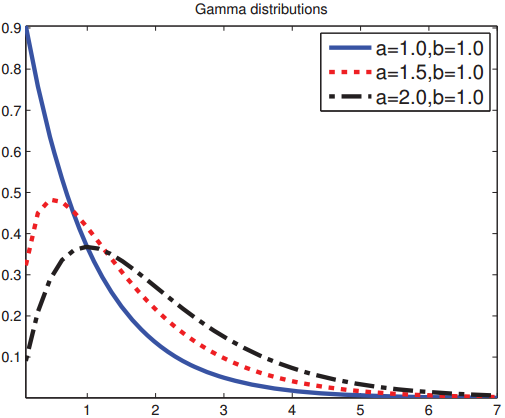
\includegraphics[scale=.50]{gamma-distribution-a.png}} \\
\subfloat[]{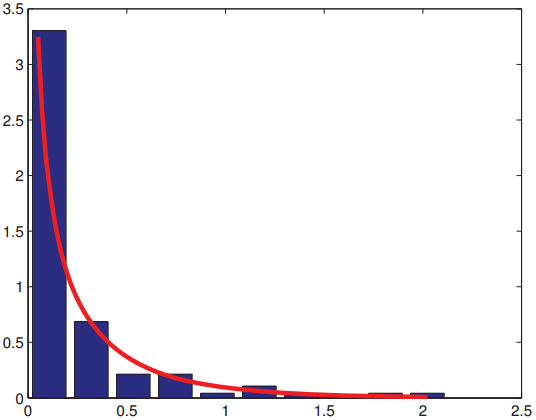
\includegraphics[scale=.50]{gamma-distribution-b.png}}
\caption{Some Ga$(a, b=1)$ distributions. If $a \leq 1$, the mode is at 0, otherwise it is $>0$.As we increase the rate $b$, we reduce the horizontal scale, thus squeezing everything leftwards and upwards. (b) An empirical pdf of some rainfall data, with a fitted Gamma distribution superimposed.}
\label{fig:gamma-distribution} 
\end{figure}


\subsection{The beta distribution}

\begin{table*}
\caption{Summary of Beta distribution}\label{tab:beta-distribution}
\centering
\begin{tabular}{ccccccc}
\hline\noalign{\smallskip}
Name & Written as & $X$ & $f(x)$ & $\mathbb{E}[X]$ & mode & $\text{var}[X]$ \\
\noalign{\smallskip}\svhline\noalign{\smallskip}
Beta distribution & $X \sim \text{Beta}(a,b)$ & $x \in [0,1]$ & $\dfrac{1}{B(a,b)}x^{a-1}(1-x)^{b-1}$ & $\dfrac{a}{a+b}$ & $\dfrac{a-1}{a+b-2}$ & $\dfrac{ab}{(a+b)^2(a+b+1)}$ \\
\noalign{\smallskip}\hline
\end{tabular}
\end{table*} 

Here $B(a, b)$is the beta function,
\begin{equation}
B(a,b) \triangleq \dfrac{\Gamma(a)\Gamma(b)}{\Gamma(a+b)}
\end{equation}

See Figure \ref{fig:beta-distribution} for plots of some beta distributions. We require  $a, b >0$ to ensure the distribution is integrable (i.e., to ensure $B(a, b)$ exists). If $a=b=1$, we get the uniform distirbution. If $a$ and $b$ are both less than 1, we get a bimodal distribution with “spikes” at 0 and 1; if $a$ and $b$ are both greater than 1, the distribution is unimodal.

\begin{figure}[hbtp]
\centering
    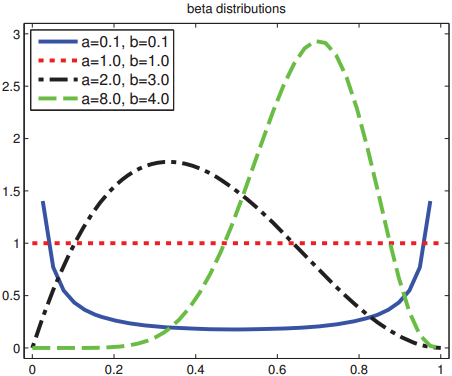
\includegraphics[scale=.60]{beta-distribution.png}
\caption{Some beta distributions.}
\label{fig:beta-distribution} 
\end{figure}


\subsection{Pareto distribution}

\begin{table*}
\caption{Summary of Pareto distribution}
\centering
\begin{tabular}{ccccccc}
\hline\noalign{\smallskip}
Name & Written as & $X$ & $f(x)$ & $\mathbb{E}[X]$ & mode & $\text{var}[X]$ \\
\noalign{\smallskip}\svhline\noalign{\smallskip}
Pareto distribution & $X \sim \text{Pareto}(k,m)$ & $x \geq m$ & $km^kx^{-(k+1)}\mathbb{I}(x \geq m)$ & $\dfrac{km}{k-1} \text{ if } k > 1$ & $m$ & $\dfrac{m^2k}{(k-1)^2(k-2)} \text{ if } k>2$ \\
\noalign{\smallskip}\hline
\end{tabular}
\end{table*} 

The \textbf{Pareto distribution} is used to model the distribution of quantities that exhibit \textbf{long tails}, also called \textbf{heavy tails}.

As $k \rightarrow \infty$, the distribution approaches $\delta(x-m)$. See Figure \ref{fig:Pareto-distribution}(a) for some plots. If we plot the distribution on a log-log scale, it forms a straight line, of the form $\log p(x)=a\log x+c$ for some constants $a$ and $c$. See Figure \ref{fig:Pareto-distribution}(b) for an illustration (this is known as a \textbf{power law}).

\begin{figure}[hbtp]
\centering
\subfloat[]{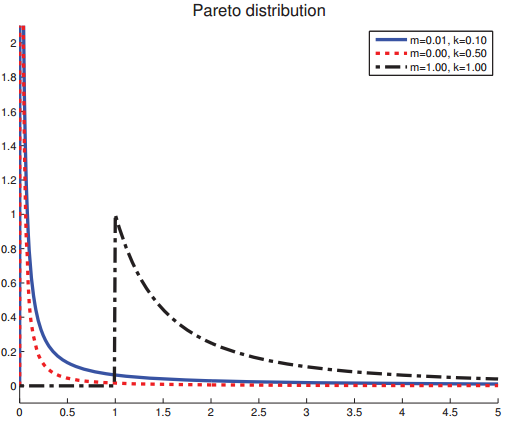
\includegraphics[scale=.50]{Pareto-distribution-a.png}} \\
\subfloat[]{\includegraphics[scale=.50]{Pareto-distribution-b.png}}
\caption{(a) The Pareto distribution Pareto$(x|m, k)$ for $m=1$. (b) The pdf on a log-log scale.}
\label{fig:Pareto-distribution} 
\end{figure}


\section{Joint probability distributions}
Given a \textbf{multivariate random variable} or \textbf{random vector} \footnote{\url{http://en.wikipedia.org/wiki/Multivariate_random_variable}} $X \in \mathbb{R}^D$, the \textbf{joint probability distribution}\footnote{\url{http://en.wikipedia.org/wiki/Joint_probability_distribution}} is a probability distribution that gives the probability that each of $X_1, X_2, \cdots,X_D$ falls in any particular range or discrete set of values specified for that variable. In the case of only two random variables, this is called a \textbf{bivariate distribution}, but the concept generalizes to any number of random variables, giving a \textbf{multivariate distribution}.

The joint probability distribution can be expressed either in terms of a \textbf{joint cumulative distribution function} or in terms of a \textbf{joint probability density function} (in the case of continuous variables) or \textbf{joint probability mass function} (in the case of discrete variables). 


\subsection{Covariance and correlation}
\begin{definition}
The \textbf{covariance} between two rv’s $X$ and $Y$ measures the degree to which $X$ and $Y$ are (linearly) related. Covariance is defined as
\begin{equation}
\begin{split}
\mathrm{cov}[X,Y] & \triangleq \mathbb{E}\left[(X-\mathbb{E}[X])(Y-\mathbb{E}[Y])\right] \\
         & =\mathbb{E}[XY]-\mathbb{E}[X]\mathbb{E}[Y]
\end{split}
\end{equation}
\end{definition}

\begin{definition}
If $X$ is a $D$-dimensional random vector, its \textbf{covariance matrix} is defined to be the following symmetric, positive definite matrix:
\begin{align}
\mathrm{cov}[X] & \triangleq \mathbb{E}\left[(X-\mathbb{E}[X])(X-\mathbb{E}[X])^T\right] \\
       &  = \left( \begin{array}{cccc}
           \text{var}[X_1] & \text{Cov}[X_1,X_2] & \cdots & \text{Cov}[X_1,X_D] \\
           \text{Cov}[X_2,X_1] & \text{var}[X_2] & \cdots & \text{Cov}[X_2,X_D] \\
		   \vdots & \vdots & \ddots & \vdots \\
           \text{Cov}[X_D,X_1] & \text{Cov}[X_D,X_2] & \cdots & \text{var}[X_D] \end{array} \right)
\end{align}
\end{definition}

\begin{definition}
The (Pearson) \textbf{correlation coefficient} between $X$ and $Y$ is defined as
\begin{equation}
\text{corr}[X,Y] \triangleq \dfrac{\text{Cov}[X,Y]}{\sqrt{\text{var}[X],\text{var}[Y]}}
\end{equation}
\end{definition}

A \textbf{correlation matrix} has the form
\begin{equation}
\mathbf{R} \triangleq \left( \begin{array}{cccc}
           \text{corr}[X_1,X_1] & \text{corr}[X_1,X_2] & \cdots & \text{corr}[X_1,X_D] \\
           \text{corr}[X_2,X_1] & \text{corr}[X_2,X_2] & \cdots & \text{corr}[X_2,X_D] \\
		   \vdots & \vdots & \ddots & \vdots \\
           \text{corr}[X_D,X_1] & \text{corr}[X_D,X_2] & \cdots & \text{corr}[X_D,X_D] \end{array} \right)
\end{equation}

The correlation coefficient can viewed as a degree of linearity between $X$ and $Y$, see Figure \ref{fig:Correlation-examples}.
\begin{figure*}[hbtp]
\centering
    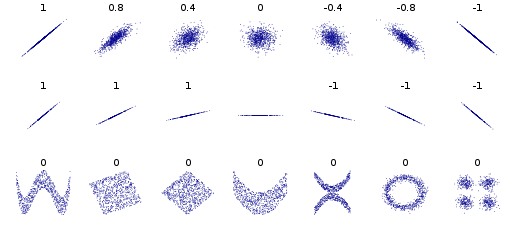
\includegraphics[scale=.80]{Correlation-examples.png}
\caption{Several sets of $(x, y)$ points, with the Pearson correlation coefficient of $x$ and $y$ for each set. Note that the correlation reflects the noisiness and direction of a linear relationship (top row), but not the slope of that relationship (middle), nor many aspects of nonlinear relationships (bottom). N.B.: the figure in the center has a slope of 0 but in that case the correlation coefficient is undefined because the variance of $Y$ is zero.Source:\url{http://en.wikipedia.org/wiki/Correlation}}
\label{fig:Correlation-examples} 
\end{figure*}

\textbf{Uncorrelated does not imply independent}. For example, let $X \sim U(-1,1)$ and $Y =X^2$. Clearly $Y$ is dependent on $X$(in fact, $Y$ is uniquely determined by $X$), yet one can show that corr$[X, Y]=0$. Some striking examples of this fact are shown in Figure \ref{fig:Correlation-examples}. This shows several data sets where there is clear dependence between $X$ and $Y$, and yet the correlation coefficient is 0. A more general measure of dependence between random variables is mutual information, see Section TODO.


\subsection{Multivariate Gaussian distribution}
\label{sec:MVN}
The \textbf{multivariate Gaussian} or \textbf{multivariate normal}(MVN) is the most widely used joint probability density function for continuous variables. We discuss MVNs in detail in Chapter 4; here we just give some definitions and plots.

The pdf of the MVN in $D$ dimensions is defined by the following:
\begin{equation}
\mathcal{N}(\vec{x}|\vec{\mu},\Sigma) \triangleq \dfrac{1}{(2\pi)^{D/2}|\Sigma|^{1/2}}\exp\left[-\dfrac{1}{2}(\vec{x}-\vec{\mu})^T\Sigma^{-1}(\vec{x}-\vec{\mu})\right]
\end{equation}
where $\vec{\mu}=\mathbb{E}[X] \in \mathbb{R}^D$ is the mean vector, and $\Sigma=\text{Cov}[X]$ is the $D \times D$ covariance matrix. The normalization constant $(2\pi)^{D/2}|\Sigma|^{1/2}$ just ensures that the pdf integrates to 1.

Figure \ref{fig:2d-Gaussions} plots some MVN densities in 2d for three different kinds of covariance matrices. A full covariance matrix has A $D(D+1)/2$ parameters (we divide by 2 since $\Sigma$ is symmetric). A diagonal covariance matrix has $D$ parameters, and has 0s in the off-diagonal terms. A spherical or isotropic covariance,$\Sigma=\sigma^2\vec{I}_D$, has one free parameter.

\begin{figure}[hbtp]
\centering
\subfloat[]{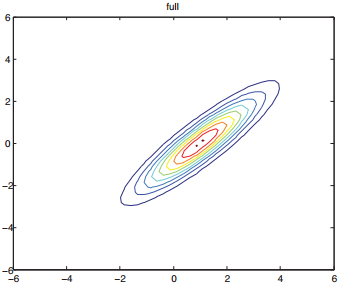
\includegraphics[scale=.60]{2d-Gaussions-a.png}} \\
\subfloat[]{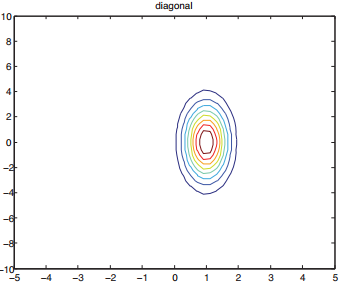
\includegraphics[scale=.60]{2d-Gaussions-b.png}} \\
\subfloat[]{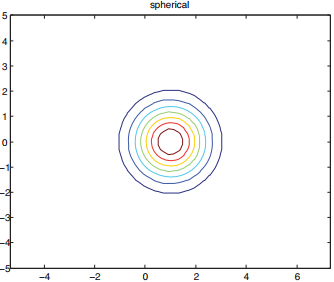
\includegraphics[scale=.60]{2d-Gaussions-c.png}} \\
\subfloat[]{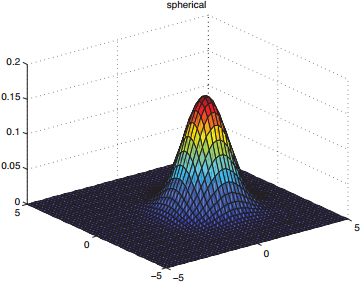
\includegraphics[scale=.60]{2d-Gaussions-d.png}}
\caption{We show the level sets for 2d Gaussians. (a) A full covariance matrix has elliptical contours.(b) A diagonal covariance matrix is an axis aligned ellipse. (c) A spherical covariance matrix has a circular shape. (d) Surface plot for the spherical Gaussian in (c).}
\label{fig:2d-Gaussions} 
\end{figure}


\subsection{Multivariate Student's t-distribution}
A more robust alternative to the MVN is the multivariate Student's t-distribution, whose pdf is given by
\begin{align}
& \mathcal{T}(x|\vec{\mu},\Sigma,\nu) \nonumber \\
& \triangleq \dfrac{\Gamma(\frac{\nu+D}{2})}{\Gamma(\frac{\nu}{2})}\dfrac{|\Sigma|^{-\frac{1}{2}}}{\left(\nu\pi\right)^{\frac{D}{2}}}\left[1+\dfrac{1}{\nu}\left(\vec{x}-\vec{\mu}\right)^T\Sigma^{-1}\left(\vec{x}-\vec{\mu}\right)\right]^{-\frac{\nu+D}{2}} \\
&= \dfrac{\Gamma(\frac{\nu+D}{2})}{\Gamma(\frac{\nu}{2})}\dfrac{|\Sigma|^{-\frac{1}{2}}}{\left(\nu\pi\right)^{\frac{D}{2}}}\left[1+\left(\vec{x}-\vec{\mu}\right)^T\vec{V}^{-1}\left(\vec{x}-\vec{\mu}\right)\right]^{-\frac{\nu+D}{2}}
\end{align}
where $\Sigma$ is called the scale matrix (since it is not exactly the covariance matrix) and $\vec{V}=\nu\Sigma$. This has fatter tails than a Gaussian. The smaller $\nu$ is, the fatter the tails. As $\nu \rightarrow \infty$, the distribution tends towards a Gaussian. The distribution has the following properties
\begin{equation}
\text{mean}=\vec{\mu} \text{ , mode}=\vec{\mu} \text{ , Cov}= \dfrac{\nu}{\nu-2}\Sigma
\end{equation}


\subsection{Dirichlet distribution}
A multivariate generalization of the beta distribution is the \textbf{Dirichlet distribution}, which has
support over the probability simplex, defined by
\begin{equation}
S_K=\left\{\vec{x}:0 \leq x_k \leq 1,\sum\limits_{k=1}^K x_k=1\right\}
\end{equation}

The pdf is defined as follows:
\begin{equation}
\text{Dir}(\vec{x}|\vec{\alpha}) \triangleq \dfrac{1}{B(\vec{\alpha})}\prod\limits_{k=1}^K x_k^{\alpha_k-1}\mathbb{I}(\vec{x} \in S_K)
\end{equation}
where $B(\alpha_1,\alpha_2,\cdots,\alpha_K)$ is the natural generalization of the beta function to $K$ variables:
\begin{equation}
B(\alpha) \triangleq \dfrac{\prod_{k=1}^K \Gamma(\alpha_k)}{\Gamma(\alpha_0)} \text{ where } \alpha_0 \triangleq \sum_{k=1}^K \alpha_k
\end{equation}

Figure \ref{fig:3d-Dirichlet} shows some plots of the Dirichlet when $K=3$, and Figure \ref{fig:5d-Dirichlet} for some sampled probability vectors. We see that $\alpha_0$ controls the strength of the distribution (how peaked it is), and theαkcontrol where the peak occurs. For example, Dir$(1,1,1)$ is a uniform distribution, Dir$(2,2,2)$ is a broad distribution centered at $(1/3,1/3,1/3)$, and Dir$(20,20,20)$ is a narrow distribution centered at $(1/3,1/3,1/3)$.If $\alpha_k < 1$ for all $k$, we get “spikes” at the corner of the simplex.

\begin{figure}[hbtp]
\centering
\subfloat[]{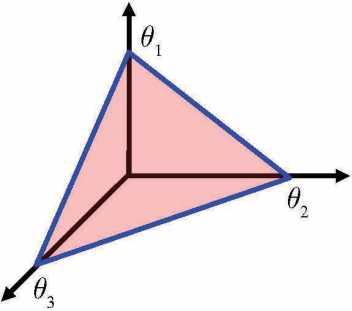
\includegraphics[scale=.50]{3d-Dirichlet-a.png}} \\
\subfloat[]{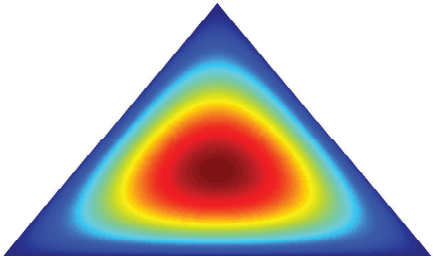
\includegraphics[scale=.60]{3d-Dirichlet-b.png}} \\
\subfloat[]{
\includegraphics[scale=.60]{3d-Dirichlet-c.png}} \\
\subfloat[]{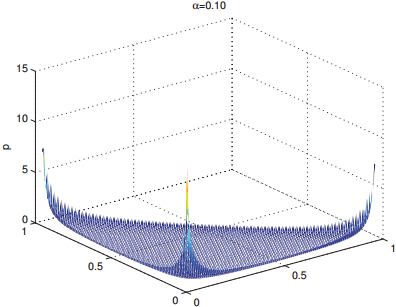
\includegraphics[scale=.60]{3d-Dirichlet-d.png}}
\caption{(a) The Dirichlet distribution when $K=3$ defines a distribution over the simplex, which can be represented by the triangular surface. Points on this surface satisfy $0 \leq \theta_k \leq 1$ and $\sum_{k=1}^K \theta_k=1$. (b) Plot of the Dirichlet density when $\vec{\alpha}=(2,2,2)$. (c) $\vec{\alpha}=(20,2,2)$.}
\label{fig:3d-Dirichlet} 
\end{figure}

\begin{figure}[hbtp]
\centering
\subfloat[$\vec{\alpha}=(0.1,\cdots,0.1)$. This results in very sparse distributions, with many 0s.]{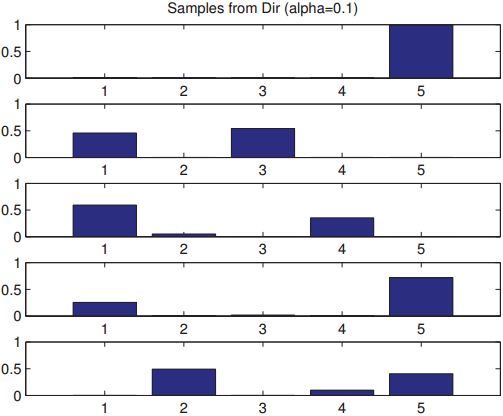
\includegraphics[scale=.50]{5d-Dirichlet-a.png}} \\
\subfloat[$\vec{\alpha}=(1,\cdots,1)$. This results in more uniform (and dense) distributions.]{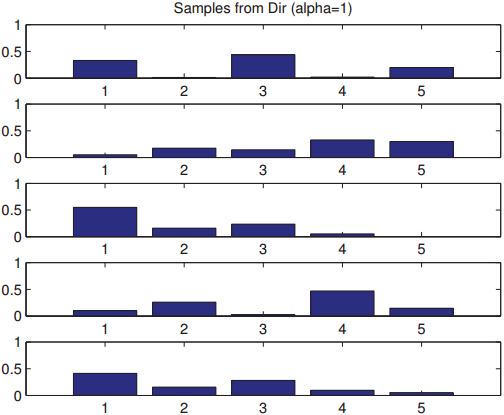
\includegraphics[scale=.50]{5d-Dirichlet-b.png}}
\caption{Samples from a 5-dimensional symmetric Dirichlet distribution for different parameter values.} 
\label{fig:5d-Dirichlet} 
\end{figure}

For future reference, the distribution has these properties
\begin{equation}\label{eqn:Dirichlet-properties}
\mathbb{E}(x_k)=\dfrac{\alpha_k}{\alpha_0} \text{, mode}[x_k]=\dfrac{\alpha_k-1}{\alpha_0-K} \text{, var}[x_k]=\dfrac{\alpha_k(\alpha_0-\alpha_k)}{\alpha_0^2(\alpha_0+1)}
\end{equation}


\section{Transformations of random variables}
If $\vec{x} \sim P()$ is some random variable, and $\vec{y}=f(\vec{x})$, what is the distribution of $Y$? This is the question we address in this section.


\subsection{Linear transformations}
Suppose $g()$ is a linear function: 
\begin{equation}
g(\vec{x})=A\vec{x}+b
\end{equation}

First, for the mean, we have
\begin{equation}
\mathbb{E}[\vec{y}]=\mathbb{E}[A\vec{x}+b]=A\mathbb{E}[\vec{x}]+b
\end{equation}
this is called the \textbf{linearity of expectation}.

For the covariance, we have
\begin{equation}
\text{Cov}[\vec{y}]=\text{Cov}[A\vec{x}+b]=A\Sigma A^T
\end{equation}


\subsection{General transformations}
\label{sec:General-transformations}
If $X$ is a discrete rv, we can derive the pmf for $y$ by simply summing up the probability mass for all the $x$’s such that $f(x)=y$:
\begin{equation}\label{eqn:transformation-discrete}
p_Y(y)=\sum\limits_{x:g(x)=y}p_X(x)
\end{equation}

If $X$ is continuous, we cannot use Equation \ref{eqn:transformation-discrete} since $p_X(x)$ is a density, not a pmf, and we cannot sum up densities. Instead, we work with cdf’s, and write
\begin{equation}
F_Y(y)=P(Y \leq y)=P(g(X) \leq y)=\int\limits_{g(X) \leq y} f_X(x)\mathrm{d}x
\end{equation}

We can derive the pdf of $Y$ by differentiating the cdf:
\begin{equation}\label{eqn:General-transformations}
f_Y(y)=f_X(x)|\dfrac{dx}{dy}|
\end{equation}

This is called \textbf{change of variables} formula. We leave the proof of this as an exercise. 

For example, suppose $X \sim U(−1,1)$, and $Y=X^2$. Then $p_Y(y)=\dfrac{1}{2}y^{-\frac{1}{2}}$.


\subsubsection{Multivariate change of variables *}
Let $f$ be a function $f:\mathbb{R}^n \rightarrow \mathbb{R}^n$, and let $\vec{y}=f(\vec{x})$. Then its Jacobian matrix $\vec{J}$ is given by
\begin{equation}
\vec{J}_{\vec{x} \rightarrow \vec{y}} \triangleq \frac{\partial \vec{y}}{\partial \vec{x}} \triangleq \left(\begin{array}{ccc}
\frac{\partial y_1}{\partial x_1} & \cdots & \frac{\partial y_1}{\partial x_n} \\
\vdots & \vdots & \vdots \\
\frac{\partial y_n}{\partial x_1} & \cdots & \frac{\partial y_n}{\partial x_n}
\end{array}\right)
\end{equation}
$|\mathrm{det}(\vec{J})|$ measures how much a unit cube changes in volume when we apply $f$.

If $f$ is an invertible mapping, we can define the pdf of the transformed variables using the Jacobian of the inverse mapping $\vec{y} \rightarrow \vec{x}$:
\begin{equation}\label{eqn:Multivariate-transformation}
p_y(\vec{y})=p_x(\vec{x})|\mathrm{det}(\frac{\partial \vec{x}}{\partial \vec{y}})|=p_x(\vec{x})|\mathrm{det}(\vec{J}_{\vec{y} \rightarrow \vec{x}})|
\end{equation}


\subsection{Central limit theorem}
Given $N$ random variables $X_1,X_2,\cdots,X_N$, each variable is \textbf{independent and identically distributed}\footnote{\url{http://en.wikipedia.org/wiki/Independent_identically_distributed}}(\textbf{iid} for short), and each has the same mean $\mu$ and variance $\sigma^2$, then
\begin{equation}
\dfrac{\sum\limits_{i=1}^n X_i-N\mu}{\sqrt{N}\sigma} \sim \mathcal{N}(0,1)
\end{equation}
this can also be written as
\begin{equation}
\dfrac{\bar{X}-\mu}{\sigma/\sqrt{N}} \sim \mathcal{N}(0,1) \quad \text{, where } \bar{X} \triangleq \dfrac{1}{N}\sum\limits_{i=1}^n X_i
\end{equation}


\section{Monte Carlo approximation}
\label{sec:Monte-Carlo-approximation}
In general, computing the distribution of a function of an rv using the change of variables formula can be difficult. One simple but powerful alternative is as follows. First we generate $S$ samples from the distribution, call them $x_1,\cdots,x_S$. (There are many ways to generate such samples; one popular method, for high dimensional distributions, is called Markov chain Monte Carlo or MCMC; this will be explained in Chapter TODO.) Given the samples, we can approximate the distribution of $f(X)$ by using the empirical distribution of $\left\{f(x_s)\right\}_{s=1}^S$. This is called a \textbf{Monte Carlo approximation}\footnote{\url{http://en.wikipedia.org/wiki/Monte_Carlo_method}}, named after a city in Europe known for its plush gambling casinos.

We can use Monte Carlo to approximate the expected value of any function of a random variable. We simply draw samples, and then compute the arithmetic mean of the function applied to the samples. This can be written as follows:
\begin{equation}
\mathbb{E}[g(X)]=\int g(x)p(x)\mathrm{d}x \approx \dfrac{1}{S}\sum\limits_{s=1}^S f(x_s)
\end{equation}
where $x_s \sim p(X)$.

This is called \textbf{Monte Carlo integration}\footnote{\url{http://en.wikipedia.org/wiki/Monte_Carlo_integration}}, and has the advantage over numerical integration (which is based on evaluating the function at a fixed grid of points) that the function is only evaluated in places where there is non-negligible probability.


\section{Information theory}

\subsection{Entropy}
\label{sec:Entropy}
The entropy of a random variable $X$ with distribution $p$, denoted by $\mathbb{H}(X)$ or sometimes $\mathbb{H}(p)$, is a measure of its uncertainty. In particular, for a discrete variable with $K$ states, it is defined by
\begin{equation}
\mathbb{H}(X) \triangleq -\sum\limits_{k=1}^{K}{p(X=k)\log_2p(X=k)}
\end{equation}

Usually we use log base 2, in which case the units are called \textbf{bits}(short for binary digits). If we use log base $e$ , the units are called \textbf{nats}. 

The discrete distribution with maximum entropy is the uniform distribution (see Section XXX for a proof). Hence for a K-ary random variable, the entropy is maximized if $p(x = k)=1/K$; in this case, $\mathbb{H}(X)=\log_2K$. 

Conversely, the distribution with minimum entropy (which is zero) is any \textbf{delta-function} that puts all its mass on one state. Such a distribution has no uncertainty.


\subsection{KL divergence}
One way to measure the dissimilarity of two probability distributions, $p$ and $q$ , is known as the \textbf{Kullback-Leibler divergence}(\textbf{KL divergence})or \textbf{relative entropy}. This is defined as follows:
\begin{equation}
\mathbb{KL}(P||Q) \triangleq 
\sum\limits_{x}{p(x)\log_2\dfrac{p(x)}{q(x)}}
\end{equation}
where the sum gets replaced by an integral for pdfs\footnote{The KL divergence is not a distance, since it is asymmetric. One symmetric version of the KL divergence is the \textbf{Jensen-Shannon divergence}, defined as $JS(p_1,p_2)=0.5\mathbb{KL}(p_1||q)+0.5\mathbb{KL}(p_2||q)$,where $q=0.5p_1+0.5p_2$}. The KL divergence is only defined if P and Q both sum to 1 and if $q(x)=0$ implies $p(x)=0$ for all $x$(absolute continuity). If the quantity  $0\ln0$ appears in the formula, it is interpreted as zero because $\lim\limits_{x \to 0}x\ln x$. We can rewrite this as
\begin{equation}\begin{split}
\mathbb{KL}(p||q) & \triangleq \sum\limits_{x}{p(x)\log_2p(x)}-\sum\limits_{k=1}^{K}{p(x)\log_2q(x)} \\
    & =\mathbb{H}(p)-\mathbb{H}(p,q)
\end{split}\end{equation}
where $\mathbb{H}(p,q)$ is called the \textbf{cross entropy},
\begin{equation}\label{eqn:cross-entropy}
\mathbb{H}(p,q)=\sum\limits_{x}{p(x)\log_2q(x)}
\end{equation}

One can show (Cover and Thomas 2006) that the cross entropy is the average number of bits needed to encode data coming from a source with distribution $p$ when we use model $q$ to define our codebook. Hence the “regular” entropy $\mathbb{H}(p)=\mathbb{H}(p,p)$, defined in section \S \ref{sec:Entropy},is the expected number of bits if we use the true model, so the KL divergence is the diference between these. In other words, the KL divergence is the average number of \emph{extra} bits needed to encode the data, due to the fact that we used distribution $q$ to encode the data instead of the true distribution $p$.

The “extra number of bits” interpretation should make it clear that $\mathbb{KL}(p||q) \geq 0$, and that the KL is only equal to zero if $q = p$. We now give a proof of this important result.

\begin{theorem}
(\textbf{Information inequality}) $\mathbb{KL}(p||q) \geq 0 \text{ with equality iff } p=q$.
\end{theorem}

One important consequence of this result is that \emph{the discrete distribution with the maximum
entropy is the uniform distribution}.


\subsection{Mutual information}
\label{sec:Mutual-information}
\begin{definition}
\textbf{Mutual information} or \textbf{MI}, is defined as follows:
\begin{equation}\begin{split}
\mathbb{I}(X;Y) & \triangleq \mathbb{KL}(P(X,Y)||P(X)P(X)) \\
    & =\sum\limits_x\sum\limits_yp(x,y)\log\dfrac{p(x,y)}{p(x)p(y)}
\end{split}\end{equation}
We have $\mathbb{I}(X;Y) \geq 0$ with equality if $P(X,Y)=P(X)P(Y)$. That is, the MI is zero if the variables are independent.
\end{definition}

To gain insight into the meaning of MI, it helps to re-express it in terms of joint and conditional entropies. One can show that the above expression is equivalent to the following:
\begin{eqnarray}
\mathbb{I}(X;Y)&=&\mathbb{H}(X)-\mathbb{H}(X|Y)\\
               &=&\mathbb{H}(Y)-\mathbb{H}(Y|X)\\
               &=&\mathbb{H}(X)+\mathbb{H}(Y)-\mathbb{H}(X,Y)\\
               &=&\mathbb{H}(X,Y)-\mathbb{H}(X|Y)-\mathbb{H}(Y|X)
\end{eqnarray}
where $\mathbb{H}(X)$ and $\mathbb{H}(Y)$ are the \textbf{marginal entropies}, $\mathbb{H}(X|Y)$ and $\mathbb{H}(Y|X)$ are the \textbf{conditional entropies}, and $\mathbb{H}(X,Y)$ is the \textbf{joint entropy} of $X$ and $Y$, see Fig. \ref{fig:mi}\footnote{\url{http://en.wikipedia.org/wiki/Mutual_information}}.

\begin{figure}[hbtp]
\centering
    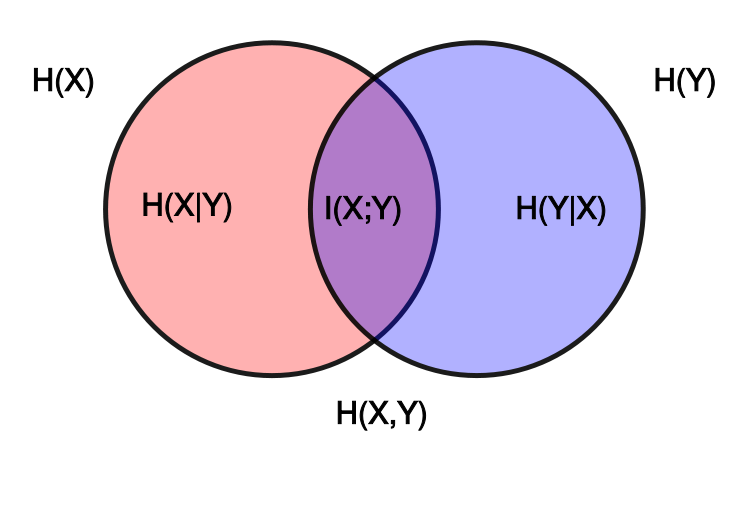
\includegraphics[scale=.25]{mutual-information.png}
\caption{Individual $\mathbb{H}(X),\mathbb{H}(Y)$, joint $\mathbb{H}(X,Y)$, and conditional entropies for a pair of correlated subsystems $X,Y$ with mutual information $\mathbb{I}(X;Y)$.}
\label{fig:mi} 
\end{figure}

Intuitively, we can interpret the MI between $X$ and $Y$ as the reduction in uncertainty about $X$ after observing $Y$, or, by symmetry, the reduction in uncertainty about $Y$ after observing $X$.

A quantity which is closely related to MI is the \textbf{pointwise mutual information} or \textbf{PMI}. For two events (not random variables) $x$ and $y$, this is defined as
\begin{equation}
PMI(x,y) \triangleq \log\dfrac{p(x,y)}{p(x)p(y)}=\log\dfrac{p(x|y)}{p(x)}=\log\dfrac{p(y|x)}{p(y)}
\end{equation}

This measures the discrepancy between these events occuring together compared to what would be expected by chance. Clearly the MI of $X$ and $Y$ is just the expected value of the PMI. Interestingly, we can rewrite the PMI as follows:
\begin{equation}
PMI(x,y)=\log\dfrac{p(x|y)}{p(x)}=\log\dfrac{p(y|x)}{p(y)}
\end{equation}

This is the amount we learn from updating the prior $p(x)$ into the posterior $p(x|y)$ , or equivalently, updating the prior $p(y)$ into the posterior $p(y |x)$ .
\chapter{Generative models for discrete data}

\section{Generative classifier}
\begin{equation}\label{eqn:Generative-classifier}
p(y=c|\vec{x},\vec{\theta})=\dfrac{p(y=c|\vec{\theta})p(\vec{x}|y=c,\vec{\theta})}{\sum_{c'}{p(y=c'|\vec{\theta})p(\vec{x}|y=c',\vec{\theta})}}
\end{equation}

This is called a \textbf{generative classifier}, since it specifies how to generate the data using the \textbf{class conditional density} $p(\vec{x}|y=c)$ and the class prior $p(y=c)$. An alternative approach is to directly fit the class posterior, $p(y=c|\vec{x})$ ;this is known as a \textbf{discriminative classifier}. 


\section{Bayesian concept learning}
Psychological research has shown that people can learn concepts from positive examples alone (Xu and Tenenbaum 2007).

We can think of learning the meaning of a word as equivalent to \textbf{concept learning}, which in turn is equivalent to binary classification. To see this, define $f(\vec{x})=1$ if xis an example of the concept $C$, and $f(\vec{x})=0$ otherwise. Then the goal is to learn the indicator function $f$, which just defines which elements are in the set $C$.


\subsection{Likelihood}
\begin{equation}
p(\mathcal{D}|h) \triangleq \left(\dfrac{1}{\text{size}(h)}\right)^N=\left(\dfrac{1}{|h|}\right)^N
\end{equation}

This crucial equation embodies what Tenenbaum calls the \textbf{size principle}, which means the model favours the simplest (smallest) hypothesis consistent with the data. This is more commonly known as \textbf{Occam’s razor}\footnote{\url{http://en.wikipedia.org/wiki/Occam\%27s_razor}}.


\subsection{Prior}
The prior is decided by human, not machines, so it is subjective. The subjectivity of the prior is controversial. For example, that a child and a math professor will reach different answers. In fact, they presumably not only have different priors, but also different hypothesis spaces. However, we can finesse that by defining the hypothesis space of the child and the math professor to be the same, and then setting the child’s prior weight to be zero on certain “advanced” concepts. Thus there is no sharp distinction between the prior and the hypothesis space.

However, the prior is the mechanism by which background knowledge can be brought to bear on a problem. Without this, rapid learning (i.e., from small samples sizes) is impossible.


\subsection{Posterior}
The posterior is simply the likelihood times the prior, normalized.
\begin{equation}
p(h|\mathcal{D}) \triangleq \dfrac{p(\mathcal{D}|h)p(h)}{\sum_{h' \in \mathcal{H}}p(\mathcal{D}|h')p(h')}=\dfrac{\mathbb{I}(\mathcal{D} \in h)p(h)}{\sum_{h' \in \mathcal{H}}\mathbb{I}(\mathcal{D} \in h')p(h')}
\end{equation}
where $\mathbb{I}(\mathcal{D} \in h)p(h)$ is 1 \textbf{iff}(iff and only if) all the data are in the extension of the hypothesis $h$.

In general, when we have enough data, the posterior $p(h|\mathcal{D})$ becomes peaked on a single concept, namely the MAP estimate, i.e.,
\begin{equation}
p(h|\mathcal{D}) \rightarrow \hat{h}^{MAP}
\end{equation}
where $\hat{h}^{MAP}$ is the posterior mode,
\begin{equation}\begin{split}
\hat{h}^{MAP} & \triangleq \arg\max\limits_h p(h|\mathcal{D})=\arg\max\limits_h p(\mathcal{D}|h)p(h) \\
    & =\arg\max\limits_h [\log p(\mathcal{D}|h) + \log p(h)]
\end{split}\end{equation}

Since the likelihood term depends exponentially on $N$, and the prior stays constant, as we get more and more data, the MAP estimate converges towards the \textbf{maximum likelihood estimate} or \textbf{MLE}:
\begin{equation}
\hat{h}^{MLE} \triangleq \arg\max\limits_h p(\mathcal{D}|h)=\arg\max\limits_h \log p(\mathcal{D}|h)
\end{equation}

In other words, if we have enough data, we see that the \textbf{data overwhelms the prior}.


\subsection{Posterior predictive distribution}
The concept of \textbf{posterior predictive distribution}\footnote{\url{http://en.wikipedia.org/wiki/Posterior_predictive_distribution}} is normally used in a Bayesian context, where it makes use of the entire posterior distribution of the parameters given the observed data to yield a probability distribution over an interval rather than simply a point estimate. 
\begin{equation}
p(\tilde{\vec{x}}|\mathcal{D}) \triangleq \mathbb{E}_{h|\mathcal{D}}[p(\tilde{\vec{x}}|h)] = \begin{cases}
\sum_h p(\tilde{\vec{x}}|h)p(h|\mathcal{D}) \\
\int p(\tilde{\vec{x}}|h)p(h|\mathcal{D})\mathrm{d}h
\end{cases}
\end{equation}

This is just a weighted average of the predictions of each individual hypothesis and is called \textbf{Bayes model averaging}(Hoeting et al. 1999). 


\section{The beta-binomial model}


\subsection{Likelihood}
Given $X \sim \text{Bin}(\theta)$, the likelihood of $\mathcal{D}$ is given by
\begin{equation}
p(\mathcal{D}|\theta)= \text{Bin}(N_1|N,\theta)
\end{equation}


\subsection{Prior}
\begin{equation}
\text{Beta}(\theta|a,b) \propto \theta^{a-1}(1-\theta)^{b-1}
\end{equation}

The parameters of the prior are called \textbf{hyper-parameters}.


\subsection{Posterior}
\begin{equation}\begin{split}\label{eqn:beta-binomial-posterior}
p(\theta|\mathcal{D}) & \propto \text{Bin}(N_1|N_1+N_0,\theta)\text{Beta}(\theta|a,b) \\
    & =\text{Beta}(\theta|N_1+a,N_0b)
\end{split}\end{equation}

Note that updating the posterior sequentially is equivalent to updating in a single batch. To see this, suppose we have two data sets $\mathcal{D}_a$ and $\mathcal{D}_b$ with sufficient statistics $N_1^a,N_0^a$ and $N_1^b,N_0^b$. Let $N_1=N_1^a+N_1^b$ and $N_0=N_0^a+N_0^b$ be the sufficient statistics of the combined datasets. In batch mode we have
\begin{align*}
p(\theta|\mathcal{D}_a,\mathcal{D}_b)& = p(\theta,\mathcal{D}_b|\mathcal{D}_a)p(\mathcal{D}_a) \\
               &\propto p(\theta,\mathcal{D}_b|\mathcal{D}_a) \\
               & = p(\mathcal{D}_b,\theta|\mathcal{D}_a) \\
			   & = p(\mathcal{D}_b|\theta)p(\theta|\mathcal{D}_a) \\
			   & \text{Combine Equation \ref{eqn:beta-binomial-posterior} and \ref{eqn:binomial-pmf}} \\
			   & =\text{Bin}(N_1^b|\theta, N_1^b+N_0^b)\text{Beta}(\theta|N_1^a+a,N_0^a+b) \\
			   & =\text{Beta}(\theta|N_1^a+N_1^b+a,N_0^a+N_0^b+b)
\end{align*}

This makes Bayesian inference particularly well-suited to \textbf{online learning}, as we will see later.

\subsubsection{Posterior mean and mode}
\label{sec:beta-binomial-Posterior-mean-and-mode}
From Table \ref{tab:beta-distribution}, the posterior mean is given by
\begin{equation}
\bar{\theta}=\dfrac{a+N_1}{a+b+N}
\end{equation}

The mode is given by
\begin{equation}
\hat{\theta}_{MAP}=\dfrac{a+N_1-1}{a+b+N-2}
\end{equation}

If we use a uniform prior, then the MAP estimate reduces to the MLE,
\begin{equation}
\hat{\theta}_{MLE}=\dfrac{N_1}{N}
\end{equation}

We will now show that the posterior mean is convex combination of the prior mean and the MLE, which captures the notion that the posterior is a compromise between what we previously believed and what the data is telling us.

\subsubsection{Posterior variance}
The mean and mode are point estimates, but it is useful to know how much we can trust them. The variance of the posterior is one way to measure this. The variance of the Beta posterior is given by
\begin{equation}
\text{var}(\theta|\mathcal{D})=\dfrac{(a+N_1)(b+N_0)}{(a+N_1+b+N_0)^2(a+N_1+b+N_0+1)}
\end{equation}

We can simplify this formidable expression in the case that $N \gg a, b$, to get
\begin{equation}
\text{var}(\theta|\mathcal{D}) \approx \dfrac{N_1N_0}{NNN}=\dfrac{\hat{\theta}_{MLE}(1-\hat{\theta}_{MLE})}{N}
\end{equation}


\subsection{Posterior predictive distribution}
So far, we have been focusing on inference of the unknown parameter(s). Let us now turn our attention to prediction of future observable data.

Consider predicting the probability of heads in a single future trial under a Beta$(a, b)$posterior. We have
\begin{align}
p(\tilde{x}|\mathcal{D})& =\int_0^1 p(\tilde{x}|\theta)p(\theta|\mathcal{D})\mathrm{d}\theta \nonumber \\
                        & =\int_0^1 \theta\text{Beta}(\theta|a,b)\mathrm{d}\theta \nonumber \\
						& =\mathbb{E}[\theta|\mathcal{D}]=\dfrac{a}{a+b}
\end{align}

\subsubsection{Overfitting and the black swan paradox}
Let us now derive a simple Bayesian solution to the problem. We will use a uniform prior, so $a=b=1$. In this case, plugging in the posterior mean gives \textbf{Laplace’s rule of succession}
\begin{equation}
p(\tilde{x}|\mathcal{D})=\dfrac{N_1+1}{N_0+N_1+1}
\end{equation}

This justifies the common practice of adding 1 to the empirical counts, normalizing and then plugging them in, a technique known as \textbf{add-one smoothing}. (Note that plugging in the MAP parameters would not have this smoothing effect, since the mode becomes the MLE if $a=b=1$, see Section \ref{sec:beta-binomial-Posterior-mean-and-mode}.)

\subsubsection{Predicting the outcome of multiple future trials}
Suppose now we were interested in predicting the number of heads, $\tilde{x}$, in $M$ future trials. This is given by
\begin{align}
p(\tilde{x}|\mathcal{D})& =\int_0^1 \text{Bin}(\tilde{x}|M,\theta)\text{Beta}(\theta|a,b)\mathrm{d}\theta \\
                        & =\dbinom{M}{\tilde{x}}\dfrac{1}{B(a,b)}\int_0^1 \theta^{\tilde{x}}(1-\theta)^{M-\tilde{x}}\theta^{a-1}(1-\theta)^{b-1}\mathrm{d}\theta
\end{align}

We recognize the integral as the normalization constant for a Beta$(a+\tilde{x}, M−\tilde{x}+b)$ distribution. Hence
\begin{equation}
\int_0^1 \theta^{\tilde{x}}(1-\theta)^{M-\tilde{x}}\theta^{a-1}(1-\theta)^{b-1}\mathrm{d}\theta=B(\tilde{x}+a,M-\tilde{x}+b)
\end{equation}

Thus we find that the posterior predictive is given by the following, known as the (compound) \textbf{beta-binomial distribution}:
\begin{equation}
Bb(x|a,b,M) \triangleq \dbinom{M}{x}\dfrac{B(x+a,M-x+b)}{B(a,b)}
\end{equation}

This distribution has the following mean and variance
\begin{equation}
\text{mean}=M\dfrac{a}{a+b} \text{ , var}=\dfrac{Mab}{(a+b)^2}\dfrac{a+b+M}{a+b+1}
\end{equation}

This process is illustrated in Figure \ref{fig:beta-binomial-distribution}. We start with a Beta$(2,2)$ prior, and plot the posterior predictive density after seeing $N_1 =3$ heads and $N_0 =17$ tails. Figure \ref{fig:beta-binomial-distribution}(b) plots a plug-in approximation using a MAP estimate. We see that the Bayesian prediction has longer tails, spreading its probability mass more widely, and is therefore less prone to overfitting and blackswan type paradoxes.

\begin{figure}[hbtp]
\centering
\subfloat[]{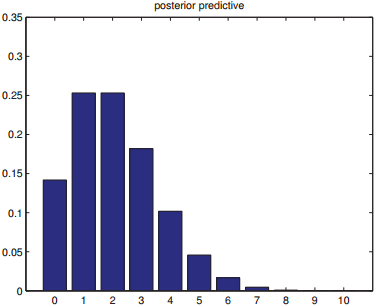
\includegraphics[scale=.60]{beta-binomial-distribution-a.png}} \\
\subfloat[]{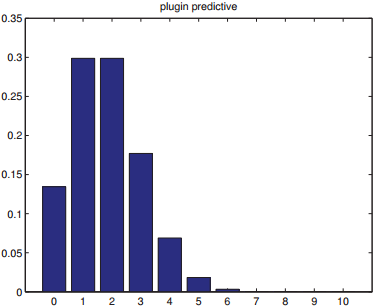
\includegraphics[scale=.60]{beta-binomial-distribution-b.png}}
\caption{(a) Posterior predictive distributions after seeing $N_1=3,N_0=17$. (b) MAP estimation.}
\label{fig:beta-binomial-distribution} 
\end{figure}


\section{The Dirichlet-multinomial model}
In the previous section, we discussed how to infer the probability that a coin comes up heads. In this section, we generalize these results to infer the probability that a dice with $K$ sides comes up as face $k$. 


\subsection{Likelihood}
Suppose we observe $N$ dice rolls, $\mathcal{D}=\{x_1,x_2,\cdots,x_N\}$, where $x_i \in \{1,2,\cdots,K\}$. The likelihood has the form
\begin{equation}
p(\mathcal{D}|\vec{\theta}) = \dbinom{N}{N_1 \cdots N_k} \prod\limits_{k=1}^K\theta_k^{N_k} \quad \text{where } N_k=\sum\limits_{i=1}^N \mathbb{I}(y_i=k)
\end{equation}
almost the same as Equation \ref{eqn:multinomial-pmf}.


\subsection{Prior}
\begin{equation}
\text{Dir}(\vec{\theta}|\vec{\alpha}) = \dfrac{1}{B(\vec{\alpha})}\prod\limits_{k=1}^K \theta_k^{\alpha_k-1}\mathbb{I}(\vec{\theta} \in S_K)
\end{equation}


\subsection{Posterior}
\begin{align}
p(\vec{\theta}|\mathcal{D})& \propto p(\mathcal{D}|\vec{\theta})p(\vec{\theta}) \\
     & \propto \prod\limits_{k=1}^K\theta_k^{N_k}\theta_k^{\alpha_k-1} = \prod\limits_{k=1}^K\theta_k^{N_k+\alpha_k-1}\\
	 & =\text{Dir}(\vec{\theta}|\alpha_1+N_1,\cdots,\alpha_K+N_K)
\end{align}

From Equation \ref{eqn:Dirichlet-properties}, the MAP estimate is given by
\begin{equation}\label{eqn:Dir-MAP}
\hat{\theta}_k=\dfrac{N_k+\alpha_k-1}{N+\alpha_0-K}
\end{equation}

If we use a uniform prior, $\alpha_k=1$, we recover the MLE:
\begin{equation}\label{eqn:Dirichlet-multinomial-posterior-MLE}
\hat{\theta}_k=\dfrac{N_k}{N}
\end{equation}


\subsection{Posterior predictive distribution}
The posterior predictive distribution for a single multinoulli trial is given by the following expression:
\begin{align}
p(X=j|\mathcal{D})& =\int p(X=j|\vec{\theta})p(\vec{\theta}|\mathcal{D})\mathrm{d}\vec{\theta} \\
    & =\int p(X=j|\theta_j)\left[\int p(\vec{\theta}_{-j}, \theta_j|\mathcal{D})\mathrm{d}\vec{\theta}_{-j}\right]\mathrm{d}\theta_j \\
	& =\int \theta_jp(\theta_j|\mathcal{D})\mathrm{d}\theta_j=\mathbb{E}[\theta_j|\mathcal{D}]=\dfrac{\alpha_j+N_j}{\alpha_0+N}
\end{align}
where $\vec{\theta}_{-j}$ are all the components of \vec{\theta} except $\theta_j$.

The above expression avoids the zero-count problem. In fact, this form of Bayesian smoothing is even more important in the multinomial case than the binary case, since the likelihood of data sparsity increases once we start partitioning the data into many categories.


\section{Naive Bayes classifiers}
\label{sec:NBC}
Assume the features are \textbf{conditionally independent} given the class label, then the class conditional density has the following form
\begin{equation}
p(\vec{x}|y,\vec{\theta})=\prod\limits_{j=1}^D p(x_j|y=c,\vec{\theta}_{jc})
\end{equation}

The resulting model is called a \textbf{naive Bayes classifier}(NBC).

The form of the class-conditional density depends on the type of each feature. We give some possibilities below:
\begin{itemize}
\item{In the case of real-valued features, we can use the Gaussian distribution: $p(\vec{x}|y,\vec{\theta})=\prod_{j=1}^D \mathcal{N}(x_j|\mu_{jc},\sigma_{jc}^2)$, where $\mu_{jc}$ is the mean of feature $j$ in objects of class $c$, and $\sigma_{jc}^2$ is its variance.}
\item{In the case of binary features, $x_j \in \{0,1\}$, we can use the Bernoulli distribution: $p(\vec{x}|y,\vec{\theta})=\prod_{j=1}^D \text{Ber}(x_j|\mu_{jc})$, where $\mu_{jc}$ is the probability that feature $j$ occurs in class $c$. This is sometimes called the \textbf{multivariate Bernoulli naive Bayes} model. We will see an application of this below.}
\item{In the case of categorical features, $x_j \in \{a_{j1},a_{j2},\cdots, a_{jS_j}\}$, we can use the multinoulli distribution: $p(\vec{x}|y,\vec{\theta})=\prod_{j=1}^D \text{Cat}(x_j|\vec{\mu}_{jc})$, where $\vec{\mu}_{jc}$ is a histogram over the $K$ possible values for $x_j$ in class $c$.}
\end{itemize}

Obviously we can handle other kinds of features, or use different distributional assumptions. Also, it is easy to mix and match features of different types.


\subsection{Optimization}
\label{sec:NBC-Optimization}
We now discuss how to “train” a naive Bayes classifier. This usually means computing the MLE or the MAP estimate for the parameters. However, we will also discuss how to compute the full posterior, $p(\vec{\theta}|\mathcal{D})$.

\subsubsection{MLE for NBC}
The probability for a single data case is given by
\begin{equation}\begin{split}
p(\vec{x}_i,y_i|\vec{\theta}) & =p(y_i|\vec{\pi})\prod\limits_j p(x_{ij}|\vec{\theta}_j) \\
  & =\prod\limits_c \pi_c^{\mathbb{I}(y_i=c)} \prod\limits_j\prod\limits_c p(x_{ij}|\vec{\theta}_{jc})^{\mathbb{I}(y_i=c)}
\end{split}\end{equation}

Hence the log-likelihood is given by
\begin{equation}
p(\mathcal{D}|\vec{\theta})=\sum\limits_{c=1}^C{N_c\log\pi_c}+ \sum\limits_{j=1}^D{\sum\limits_{c=1}^C{\sum\limits_{i:y_i=c}{\log p(x_{ij}|\vec{\theta}_{jc})}}}
\end{equation}
where $N_c \triangleq \sum\limits_i \mathbb{I}(y_i=c)$ is the number of feature vectors in class $c$.

We see that this expression decomposes into a series of terms, one concerning $\vec{\pi}$, and $DC$ terms containing the $\theta_{jc}$’s. Hence we can optimize all these parameters separately.

From Equation \ref{eqn:Dirichlet-multinomial-posterior-MLE}, the MLE for the class prior is given by
\begin{equation}
\hat{\pi}_c=\dfrac{N_c}{N}
\end{equation}

The MLE for $\theta_{jc}$’s depends on the type of distribution we choose to use for each feature. 

In the case of binary features, $x_j \in \{0,1\}$, $x_j|y=c \sim \text{Ber}(\theta_{jc})$, hence
\begin{equation}
\hat{\theta}_{jc}=\dfrac{N_{jc}}{N_c}
\end{equation}
where $N_{jc} \triangleq \sum\limits_{i:y_i=c} \mathbb{I}(y_i=c)$ is the number that feature $j$ occurs in class $c$.

In the case of categorical features, $x_j \in \{a_{j1},a_{j2},\cdots, a_{jS_j}\}$, $x_j|y=c \sim \text{Cat}(\vec{\theta}_{jc})$, hence
\begin{equation}
\hat{\vec{\theta}}_{jc}=(\dfrac{N_{j1c}}{N_c},\dfrac{N_{j2c}}{N_c}, \cdots, \dfrac{N_{jS_j}}{N_c})^T
\end{equation}
where $N_{jkc} \triangleq \sum\limits_{i=1}^N \mathbb{I}(x_{ij}=a_{jk}, y_i=c)$ is the number that feature $x_j=a_{jk}$ occurs in class $c$.


\subsubsection{Bayesian naive Bayes}
\label{sec:Bayesian-naive-Bayes}
Use a Dir$(\vec{\alpha})$ prior for $\vec{\pi}$.

In the case of binary features, use a Beta$(\beta0,\beta1)$ prior for each $\theta_{jc}$; in the case of categorical features, use a Dir$(\vec{\alpha})$ prior for each  $\vec{\theta}_{jc}$. Often we just take $\vec{\alpha}=\vec{1}$ and $\vec{\beta}=\vec{1}$, corresponding to \textbf{add-one} or \textbf{Laplace smoothing}.


\subsection{Using the model for prediction}
The goal is to compute
\begin{equation}\begin{split}
y=f(\vec{x}) & =\arg\max\limits_{c}{P(y=c|\vec{x},\vec{\theta})} \\
   & =P(y=c|\vec{\theta})\prod_{j=1}^D P(x_j|y=c,\vec{\theta})
\end{split}\end{equation}

We can the estimate parameters using MLE or MAP, then the posterior predictive density is obtained by simply plugging in the parameters $\bar{\vec{\theta}}$(MLE) or $\hat{\vec{\theta}}$(MAP). 

Or we can use BMA, just integrate out the unknown parameters.


\subsection{The log-sum-exp trick}
when using generative classifiers of any kind, computing the posterior over class labels using Equation \ref{eqn:Generative-classifier} can fail due to \textbf{numerical underflow}. The problem is that $p(\vec{x}|y=c)$ is often a very small number, especially if \vec{x} is a high-dimensional vector. This is because we require that $\sum_{\vec{x}}p(\vec{x}|y)=1$, so the probability of observing any particular high-dimensional vector is small. The obvious solution is to take logs when applying Bayes rule, as follows:
\begin{equation}
\log p(y=c|\vec{x},\vec{\theta})=b_c-\log\left(\sum\limits_{c'}e^{b_{c'}}\right)
\end{equation}
where $b_c \triangleq \log p(\vec{x}|y=c,\vec{\theta})+\log p(y=c|\vec{\theta})$.

We can factor out the largest term, and just represent the remaining numbers relative to that. For example,
\begin{equation}\begin{split}
\log(e^{-120}+e^{-121}) & =\log(e^{-120}(1+e^{-1})) \\
   & =\log(1+e^{-1})-120
\end{split}\end{equation}

In general, we have
\begin{equation}
\sum\limits_{c}e^{b_{c}}=\log\left[(\sum e^{b_c-B})e^B\right]=\log\left(\sum e^{b_c-B}\right)+B
\end{equation}
where $B \triangleq \max\{b_c\}$.

This is called the \textbf{log-sum-exp} trick, and is widely used. 


\subsection{Feature selection using mutual information}
Since an NBC is fitting a joint distribution over potentially many features, it can suffer from overfitting. In addition, the run-time cost is $O(D)$, which may be too high for some applications. 

One common approach to tackling both of these problems is to perform \textbf{feature selection}, to remove “irrelevant” features that do not help much with the classification problem. The simplest approach to feature selection is to evaluate the relevance of each feature separately, and then take the top K,whereKis chosen based on some tradeoff between accuracy and complexity. This approach is known as \textbf{variable ranking}, \textbf{filtering}, or \textbf{screening}.

One way to measure relevance is to use mutual information (Section \ref{sec:Mutual-information}) between feature $X_j$ and the class label $Y$
\begin{equation}
\mathbb{I}(X_j,Y)=\sum\limits_{x_j}{\sum\limits_{y}{p(x_j,y)\log \dfrac{p(x_j,y)}{p(x_j)p(y)}}}
\end{equation}

If the features are binary, it is easy to show that the MI can be computed as follows
\begin{equation}
\mathbb{I}_j = \sum\limits_c \left[\theta_{jc}\pi_c\log{\dfrac{\theta_{jc}}{\theta_j}}+(1-\theta_{jc})\pi_c\log{\dfrac{1-\theta_{jc}}{1-\theta_j}}\right]
\end{equation}
where $\pi_c=p(y=c)$, $\theta_{jc}=p(x_j=1|y=c)$, and $\theta_j=p(x_j=1)=\sum_{c} \pi_c\theta_{jc}$.


\subsection{Classifying documents using bag of words}
\textbf{Document classification} is the problem of classifying text documents into different categories.


\subsubsection{Bernoulli product model}
One simple approach is to represent each document as a binary vector, which records whether each word is present or not, so $x_{ij} =1$ iff word $j$ occurs in document $i$, otherwise $x_{ij}=0$. We can then use the following class conditional density:
\begin{equation}\begin{split}
p(\vec{x}_i|y_i=c,\vec{\theta}) & =\prod\limits_{j=1}^D \mathrm{Ber}(x_{ij}|\theta_{jc}) \\
  & =\prod\limits_{j=1}^D \theta_{jc}^{x_{ij}}(1-\theta_{jc})^{1-x_{ij}}
\end{split}\end{equation}

This is called the \textbf{Bernoulli product model}, or the \textbf{binary independence model}.

\subsubsection{Multinomial document classifier}
However, ignoring the number of times each word occurs in a document loses some information (McCallum and Nigam 1998). A more accurate representation counts the number of occurrences of each word. Specifically, let $\vec{x}_i$ be a vector of counts for document $i$, so $x_{ij} \in \{0,1,\cdots,N_i\}$, where $N_i$ is the number of terms in document $i$(so $\sum\limits_{j=1}^D x_{ij}=N_i$). For the class conditional densities, we can use a multinomial distribution:
\begin{equation}\label{eqn:Multinomial-document-classifier}
p(\vec{x}_i|y_i=c,\vec{\theta})=\text{Mu}(\vec{x}_i|N_i,\vec{\theta}_c)=\dfrac{N_i!}{\prod_{j=1}^D x_{ij}!}\prod\limits_{j=1}^D \theta_{jc}^{x_{ij}}
\end{equation}
where we have implicitly assumed that the document length $N_i$ is independent of the class. Here $θ_{jc}$ is the probability of generating word $j$ in documents of class $c$; these parameters satisfy the constraint that $\sum_{j=1}^D \theta_{jc}=1$ for each class c.

Although the multinomial classifier is easy to train and easy to use at test time, it does not work particularly well for document classification. One reason for this is that it does not take into account the \textbf{burstiness} of word usage. This refers to the phenomenon that most words never appear in any given document, but if they do appear once, they are likely to appear more than once, i.e., words occur in bursts.

The multinomial model cannot capture the burstiness phenomenon. To see why, note that Equation \ref{eqn:Multinomial-document-classifier} has the form $\theta_{jc}^{x_{ij}}$, and since $\theta_{jc} \ll 1$ for rare words, it becomes increasingly unlikely to generate many of them. For more frequent words, the decay rate is not as fast. To see why intuitively, note that the most frequent words are function words which are not specific to the class, such as “and”, “the”, and “but”; the chance of the word “and” occuring is pretty much the same no matter how many time it has previously occurred (modulo document length), so the independence assumption is more reasonable for common words. However, since rare words are the ones that matter most for classification purposes, these are the ones we want to model the most carefully.

\subsubsection{DCM model}
Various ad hoc heuristics have been proposed to improve the performance of the multinomial document classifier (Rennie et al. 2003). We now present an alternative class conditional density that performs as well as these ad hoc methods, yet is probabilistically sound (Madsen et al. 2005).

Suppose we simply replace the multinomial class conditional density with the \textbf{Dirichlet Compound Multinomial} or \textbf{DCM} density, defined as follows:
\begin{equation}\begin{split}
p(\vec{x}_i|y_i=c,\vec{\alpha}) & =\int \text{Mu}(\vec{x}_i|N_i,\vec{\theta}_c)\text{Dir}(\vec{\theta}_c|\vec{\alpha}_c) \\
   & =\dfrac{N_i!}{\prod_{j=1}^D x_{ij}!}\prod\limits_{j=1}^D\dfrac{B(\vec{x}_i+\vec{\alpha}_c)}{B(\vec{\alpha}_c)}
\end{split}\end{equation}

(This equation is derived in Equation TODO.) Surprisingly this simple change is all that is needed to capture the burstiness phenomenon. The intuitive reason for this is as follows: After seeing one occurence of a word, say wordj, the posterior counts on θj gets updated, making another occurence of wordjmore likely. By contrast, ifθj is fixed, then the occurences of each word are independent. The multinomial model corresponds to drawing a ball from an urn with Kcolors of ball, recording its color, and then replacing it. By contrast, the DCM model corresponds to drawing a ball, recording its color, and then replacing it with one additional copy; this is called the \textbf{Polya urn}.

Using the DCM as the class conditional density gives much better results than using the multinomial, and has performance comparable to state of the art methods, as described in (Madsen et al. 2005). The only disadvantage is that fitting the DCM model is more complex; see (Minka 2000e; Elkan 2006) for the details.

\chapter{Gaussian Models}
\label{chap:MVN}

In this chapter, we discuss the \textbf{multivariate Gaussian} or \textbf{multivariate normal(MVN)}, which is the most widely used joint probability density function for continuous variables. It will form the basis for many of the models we will encounter in later chapters.


\section{Basics}
Recall from Section ~\ref{sec:MVN} that the pdf for an MVN in $D$ dimensions is defined by the following:
\begin{equation}
\mathcal{N}(\vec{x}|\vec{\mu},\Sigma) \triangleq \dfrac{1}{(2\pi)^{D/2}|\Sigma|^{1/2}}\exp\left[-\dfrac{1}{2}(\vec{x}-\vec{\mu})^T\Sigma^{-1}(\vec{x}-\vec{\mu})\right]
\end{equation}

The expression inside the exponent is the Mahalanobis distance between a data vector $\vec{x}$ and the mean vector $\vec{\mu}$, We can gain a better understanding of this quantity by performing an \textbf{eigendecomposition} of $\vec{\Sigma}$. That is, we write $\vec{\Sigma}=\vec{U}\vec{\Lambda}\vec{U}^T$, where $\vec{U}$ is an orthonormal matrix of eigenvectors satsifying $\vec{U}^T\vec{U}=\vec{I}$, and $\vec{\Lambda}$ is a diagonal matrix of eigenvalues. Using the eigendecomposition, we have that
\begin{equation}
\vec{\Sigma}^{-1}=\vec{U}^{-T}\vec{\Lambda}^{-1}\vec{U}^{-1}=\vec{U}\vec{\Lambda}^{-1}\vec{U}^T=\sum\limits_{i=1}^D \dfrac{1}{\lambda_i}\vec{u}_i\vec{u}_i^T
\end{equation}
where $\vec{u}_i$ is the $i$’th column of $\vec{U}$, containing the $i$’th eigenvector. Hence we can rewrite the Mahalanobis distance as follows:
\begin{align}
(\vec{x}-\vec{\mu})^T\Sigma^{-1}(\vec{x}-\vec{\mu})& =(\vec{x}-\vec{\mu})^T\left(\sum\limits_{i=1}^D \dfrac{1}{\lambda_i}\vec{u}_i\vec{u}_i^T\right)(\vec{x}-\vec{\mu}) \\
    & =\sum\limits_{i=1}^D \dfrac{1}{\lambda_i}(\vec{x}-\vec{\mu})^T\vec{u}_i\vec{u}_i^T(\vec{x}-\vec{\mu})=\sum\limits_{i=1}^D \dfrac{y_i^2}{\lambda_i}
\end{align}
where $y_i \triangleq \vec{u}_i^T(\vec{x}-\vec{\mu})$. Recall that the equation for an ellipse in 2d is
\begin{equation}
\dfrac{y_1^2}{\lambda_1}+\dfrac{y_2^2}{\lambda_2}=1
\end{equation}

Hence we see that the contours of equal probability density of a Gaussian lie along ellipses. This is illustrated in Figure ~\ref{fig:2d-MVN}. The eigenvectors determine the orientation of the ellipse, and the eigenvalues determine how elogonated it is.

\begin{figure}[hbtp]
\centering
    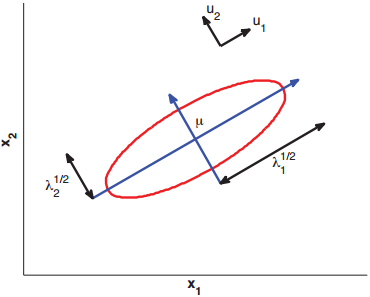
\includegraphics[scale=.70]{2d-MVN.png}
\caption{Visualization of a 2 dimensional Gaussian density. The major and minor axes of the ellipse are defined by the first two eigenvectors of the covariance matrix, namely $\vec{u}_1$ and $\vec{u}_2$. Based on Figure 2.7 of (Bishop 2006a)}
\label{fig:2d-MVN} 
\end{figure}

In general, we see that the Mahalanobis distance corresponds to Euclidean distance in a transformed coordinate system, where we shift by $\vec{\mu}$ and rotate by $\vec{U}$.


\subsection{MLE for a MVN}
\begin{theorem}(\textbf{MLE for a MVN})
If we have $N$ iid samples $\vec{x}_i \sim \mathcal{N}(\vec{\mu},\vec{\Sigma})$, then the MLE for the parameters is given by
\begin{align}
& \bar{\vec{\mu}}=\dfrac{1}{N}\sum\limits_{i=1}^N \vec{x}_i \triangleq \bar{\vec{x}} \\
& \bar{\vec{\Sigma}}=\dfrac{1}{N}\sum\limits_{i=1}^N (\vec{x}_i-\bar{\vec{x}})(\vec{x}_i-\bar{\vec{x}})^T=\dfrac{1}{N}\left(\sum\limits_{i=1}^N \vec{x}_i\vec{x}_i^T\right)-\bar{\vec{x}}\bar{\vec{x}}^T
\end{align}
\end{theorem}


\subsection{Maximum entropy derivation of the Gaussian *}
In this section, we show that the multivariate Gaussian is the distribution with maximum entropy subject to having a specified mean and covariance (see also Section TODO). This is one reason the Gaussian is so widely used: the first two moments are usually all that we can reliably estimate from data, so we want a distribution that captures these properties, but otherwise makes as few addtional assumptions as possible.

To simplify notation, we will assume the mean is zero. The pdf has the form
\begin{equation}
f(\vec{x})=\dfrac{1}{Z}\exp\left(-\dfrac{1}{2}\vec{x}^T\vec{\Sigma}^{-1}\vec{x}\right)
\end{equation}


\section{Gaussian discriminant analysis}
One important application of MVNs is to define the the class conditional densities in a generative classifier, i.e.,
\begin{equation}
p(\vec{x}|y=c,\vec{\theta})=\mathcal{N}(\vec{x}|\vec{\mu}_c,\vec{\Sigma}_c)
\end{equation}

The resulting technique is called (Gaussian) \textbf{discriminant analysis} or \textbf{GDA} (even though it is a generative, not discriminative, classifier — see Section TODO for more on this distinction). If $\vec{\Sigma}_c$ is diagonal, this is equivalent to naive Bayes.

We can classify a feature vector using the following decision rule, derived from Equation ~\eqref{eqn:Generative-classifier}:
\begin{equation}
y=\arg\max_{c} \left[\log p(y=c|\vec{\pi})+\log p(\vec{x}|\vec{\theta})\right]
\end{equation}

When we compute the probability of $\vec{x}$ under each class conditional density, we are measuring the distance from $\vec{x}$ to the center of each class, $\vec{\mu}_c$, using Mahalanobis distance. This can be thought of as a \textbf{nearest centroids classifier}.

\begin{figure}[hbtp]
\centering
    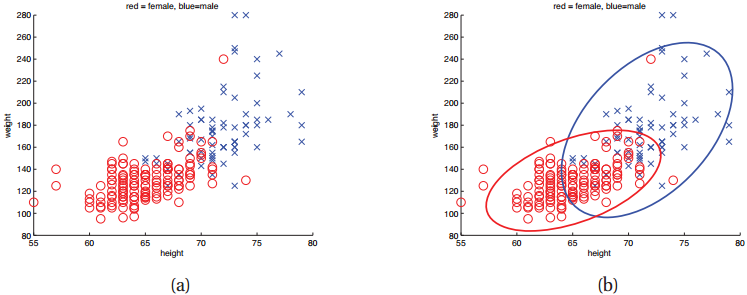
\includegraphics[scale=.70]{2d-Gaussians-Visualization.png}
\caption{(a) Height/weight data. (b) Visualization of 2d Gaussians fit to each class. 95\% of the probability mass is inside the ellipse.}
\label{fig:2d-Gaussians-Visualization} 
\end{figure}

As an example, Figure ~\ref{fig:2d-Gaussians-Visualization} shows two Gaussian class-conditional densities in 2d, representing the height and weight of men and women. We can see that the features are correlated, as is to be expected (tall people tend to weigh more). The ellipses for each class contain 95\% of the probability mass. If we have a uniform prior over classes, we can classify a new test vector as follows:
\begin{equation}
y=\arg\max_{c} (\vec{x}-\vec{\mu}_c)^T\vec{\Sigma}_c^{-1}(\vec{x}-\vec{\mu}_c)
\end{equation}


\subsection{Quadratic discriminant analysis (QDA)}
By plugging in the definition of the Gaussian density to Equation ~\eqref{eqn:Generative-classifier}, we can get
\begin{equation}\label{eqn:QDA}
p(y|\vec{x},\vec{\theta})=\dfrac{\pi_c|2\pi\vec{\Sigma}_c|^{-\frac{1}{2}}\exp\left[-\frac{1}{2}(\vec{x}-\vec{\mu})^T\vec{\Sigma}^{-1}(\vec{x}-\vec{\mu})\right]}{\sum_{c'}\pi_{c'}|2\pi\vec{\Sigma}_{c'}|^{-\frac{1}{2}}\exp\left[-\frac{1}{2}(\vec{x}-\vec{\mu})^T\vec{\Sigma}^{-1}(\vec{x}-\vec{\mu})\right]}
\end{equation}

Thresholding this results in a quadratic function ofx. The result is known as quadratic discriminant analysis(QDA). Figure ~\ref{fig:QDA} gives some examples of what the decision boundaries look like in 2D.

\begin{figure}[hbtp]
\centering
    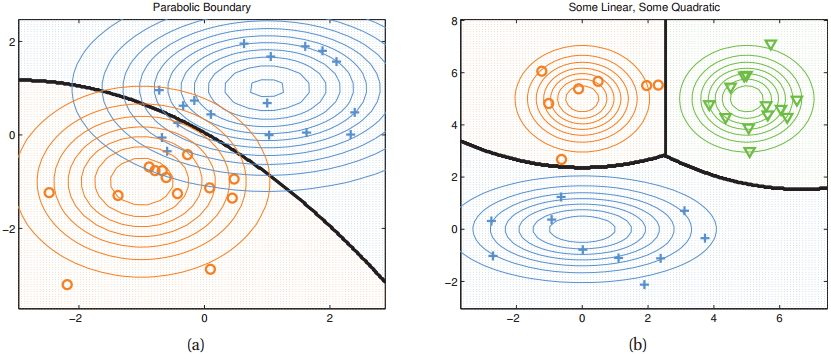
\includegraphics[scale=.60]{QDA.png}
\caption{Quadratic decision boundaries in 2D for the 2 and 3 class case.}
\label{fig:QDA} 
\end{figure}


\subsection{Linear discriminant analysis (LDA)}
\label{sec:Linear-discriminant-analysis}
We now consider a special case in which the covariance matrices are \textbf{tied} or \textbf{shared} across classes,$\vec{\Sigma}_c=\vec{\Sigma}$. In this case, we can simplify Equation ~\eqref{eqn:QDA} as follows:
\begin{align}
p(y|\vec{x},\vec{\theta})& \propto \pi_c\exp\left(\vec{\mu}_c\vec{\Sigma}^{-1}\vec{x}-\dfrac{1}{2}\vec{x}^T\vec{\Sigma}^{-1}\vec{x}-\dfrac{1}{2}\vec{\mu}_c^T\vec{\Sigma}^{-1}\vec{\mu}_c\right) \\
 & =\exp\left(\vec{\mu}_c\vec{\Sigma}^{-1}\vec{x}-\dfrac{1}{2}\vec{\mu}_c^T\vec{\Sigma}^{-1}\vec{\mu}_c+\log \pi_c\right)\exp\left(-\dfrac{1}{2}\vec{x}^T\vec{\Sigma}^{-1}\vec{x}\right) \\
 & \propto \exp\left(\vec{\mu}_c\vec{\Sigma}^{-1}\vec{x}-\dfrac{1}{2}\vec{\mu}_c^T\vec{\Sigma}^{-1}\vec{\mu}_c+\log \pi_c\right)
\end{align}

Since the quadratic term $\vec{x}^T\vec{\Sigma}^{-1}\vec{x}$ is independent of $c$, it will cancel out in the numerator and denominator. If we define
\begin{align}
\gamma_c& \triangleq -\dfrac{1}{2}\vec{\mu}_c^T\vec{\Sigma}^{-1}\vec{\mu}_c+\log \pi_c \\
\vec{\beta}_c& \triangleq \vec{\Sigma}^{-1}\vec{\mu}_c
\end{align}
then we can write
\begin{equation}\label{eqn:LDA}
p(y|\vec{x},\vec{\theta})=\dfrac{e^{\vec{\beta}_c^T\vec{x}+\gamma_c}}{\sum_{c'}e^{\vec{\beta}_{c'}^T\vec{x}+\gamma_{c'}}} \triangleq \sigma(\vec{\eta}, c) \quad \text{where } \vec{\eta} \triangleq (e^{\vec{\beta}_1^T\vec{x}}+\gamma_1,\cdots, e^{\vec{\beta}_C^T\vec{x}}+\gamma_C)
\end{equation}
where $\sigma()$ is the \textbf{softmax activation function}\footnote{\url{http://en.wikipedia.org/wiki/Softmax_activation_function}}, defined as follows:
\begin{equation}
\sigma(\vec{q},i) \triangleq \dfrac{\exp(q_i)}{\sum_{j=1}^n \exp(q_j)}
\end{equation}

When parameterized by some constant, $\alpha > 0$, the following formulation becomes a smooth, differentiable approximation of the maximum function:
\begin{equation}
\mathcal{S}_{\alpha}(\vec{x}) = \dfrac{\sum_{j=1}^D x_je^{\alpha x_j}}{\sum_{j=1}^D e^{\alpha x_j}}
\end{equation}

$\mathcal{S}_{\alpha}$ has the following properties:
\begin{enumerate}
\item $\mathcal{S}_{\alpha} \rightarrow \max$ as $\alpha \rightarrow \infty$
\item $\mathcal{S}_0$ is the average of its inputs
\item $\mathcal{S}_{\alpha} \rightarrow \min$ as $\alpha \rightarrow -\infty$
\end{enumerate}

Note that the softmax activation function comes from the area of statistical physics, where it is common to use the \textbf{Boltzmann distribution}, which has the same form as the softmax activation function.

An interesting property of Equation ~\eqref{eqn:LDA} is that, if we take logs, we end up with a linear function of $\vec{x}$. (The reason it is linear is because the $\vec{x}^T\vec{\Sigma}^{-1}\vec{x}$ cancels from the numerator and denominator.) Thus the decision boundary between any two classes, says $c$ and $c'$, will be a straight line. Hence this technique is called \textbf{linear discriminant analysis} or \textbf{LDA}.

An alternative to fitting an LDA model and then deriving the class posterior is to directly fit $p(y|\vec{x},\vec{W})=\text{Cat}(y|\vec{W}\vec{x})$ for some $C \times D$ weight matrix $\vec{W}$. This is called \textbf{multi-class logistic regression}, or \textbf{multinomial logistic regression}. We will discuss this model in detail in Section TODO. The difference between the two approaches is explained in Section TODO.


\subsection{Two-class LDA}
To gain further insight into the meaning of these equations, let us consider the binary case. In this case, the posterior is given by
\begin{align}
p(y=1|\vec{x},\vec{\theta})& =\dfrac{e^{\vec{\beta}_1^T\vec{x}+\gamma_1}}{e^{\vec{\beta}_0^T\vec{x}+\gamma_0}+e^{\vec{\beta}_1^T\vec{x}+\gamma_1}}) \\
  & =\dfrac{1}{1+e^(\vec{\beta}_0-\vec{\beta}_1)^T\vec{x}+(\gamma_0-\gamma_1)}=\text{sigm}((\vec{\beta}_1-\vec{\beta}_0)^T\vec{x}+(\gamma_0-\gamma_1))
\end{align}
where sigm$(x)$ refers to the sigmoid function\footnote{\url{http://en.wikipedia.org/wiki/Sigmoid_function}}.

Now
\begin{align}
\gamma_1-\gamma_0& = -\dfrac{1}{2}\vec{\mu}_1^T\vec{\Sigma}^{-1}\vec{\mu}_1+\dfrac{1}{2}\vec{\mu}_0^T\vec{\Sigma}^{-1}\vec{\mu}_0 + \log(\pi_1/\pi_0) \\
 & =-\dfrac{1}{2}(\vec{\mu}_1-\vec{\mu}_0)^T\vec{\Sigma}^{-1}(\vec{\mu}_1+\vec{\mu}_0)+ \log(\pi_1/\pi_0)
\end{align}

So if we define
\begin{align}
\vec{w}& =\vec{\beta}_1-\vec{\beta}_0=\vec{\Sigma}^{-1}(\vec{\mu}_1-\vec{\mu}_0) \\
\vec{x}_0& =\dfrac{1}{2}(\vec{\mu}_1+\vec{\mu}_0)-(\vec{\mu}_1-\vec{\mu}_0)\dfrac{\log(\pi_1/\pi_0)}{(\vec{\mu}_1-\vec{\mu}_0)^T\vec{\Sigma}^{-1}(\vec{\mu}_1-\vec{\mu}_0)}
\end{align}
then we have $\vec{w}^T\vec{x}_0=-(\gamma_1-\gamma_0)$, and hence
\begin{equation}
p(y=1|\vec{x},\vec{\theta})=\text{sigm}(\vec{w}^T(\vec{x}-\vec{x}_0))
\end{equation}

(This is closely related to logistic regression, which we will discuss in Section TODO.) So the final decision rule is as follows: shift $\vec{x}$ by $\vec{x}_0$, project onto the line \vec{w}, and see if the result is positive or negative.

\begin{figure}[hbtp]
\centering
    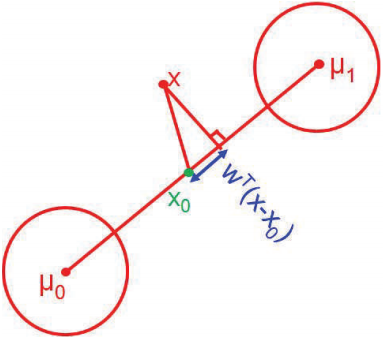
\includegraphics[scale=.60]{2d-LDA.png}
\caption{Geometry of LDA in the 2 class case where $\vec{\Sigma}_1=\vec{\Sigma}_2=\vec{I}$.}
\label{fig:2d-LDA} 
\end{figure}

If $\vec{\Sigma}=\sigma^2\vec{I}$, then $\vec{w}$ is in the direction of $\vec{\mu}_1-\vec{\mu}_0$. So we classify the point based on whether its projection is closer to $\vec{\mu}_0$ or $\vec{\mu}_1$ . This is illustrated in Figure ~\ref{fig:2d-LDA}. Furthemore, if $\vec{\pi}_1=\vec{\pi}_0$, then $\vec{x}_0=\frac{1}{2}(\vec{\mu}_1+\vec{\mu}_0)$, which is half way between the means. If we make $\vec{\pi}_1>\vec{\pi}_0$, then $\vec{x}_0$ gets closer to $\vec{\mu}_0$, so more of the line belongs to class 1 a \emph{priori}. Conversely if $\vec{\pi}_1<\vec{\pi}_0$, the boundary shifts right. Thus we see that the class prior, πc, just changes the decision threshold, and not the overall geometry, as we claimed above. (A similar argument applies in the multi-class case.)

The magnitude of $\vec{w}$ determines the steepness of the logistic function, and depends on how well-separated the means are, relative to the variance. In psychology and signal detection theory, it is common to define the \textbf{discriminability} of a signal from the background noise using a quantity called \textbf{d-prime}:
\begin{equation}
d' \triangleq \dfrac{\mu_1-\mu_0}{\sigma}
\end{equation}
where $\mu_1$ is the mean of the signal and $\mu_0$ is the mean of the noise, and $\sigma$ is the standard deviation of the noise. If $d'$ is large, the signal will be easier to discriminate from the noise.


\subsection{MLE for discriminant analysis}
\label{sec:MLE-for-discriminant-analysis}
The log-likelihood function is as follows:
\begin{equation}
p(\mathcal{D}|\vec{\theta})=\sum\limits_{c=1}^C{\sum\limits_{i:y_i=c}{\log\pi_c}}+\sum\limits_{c=1}^C{\sum\limits_{i:y_i=c}{\log\mathcal{N}(\vec{x}_i|\vec{\mu}_c,\vec{\Sigma}_c)}}
\end{equation}

The MLE for each parameter is as follows:
\begin{align}
\bar{\vec{\mu}}_c& = \dfrac{N_c}{N} \\
\bar{\vec{\mu}}_c& = \dfrac{1}{N_c}\sum\limits_{i:y_i=c}\vec{x}_i \\
\bar{\vec{\Sigma}}_c& = \dfrac{1}{N_c}\sum\limits_{i:y_i=c}(\vec{x}_i-\bar{\vec{\mu}}_c)(\vec{x}_i-\bar{\vec{\mu}}_c)^T
\end{align}


\subsection{Strategies for preventing overfitting}
The speed and simplicity of the MLE method is one of its greatest appeals. However, the MLE can badly overfit in high dimensions. In particular, the MLE for a full covariance matrix is singular if $N_c <D$. And even when $N_c >D$, the MLE can be ill-conditioned, meaning it is close to singular. There are several possible solutions to this problem:
\begin{itemize}
\item{Use a diagonal covariance matrix for each class, which assumes the features are conditionally independent; this is equivalent to using a naive Bayes classifier (Section ~\ref{sec:NBC})}.
\item{Use a full covariance matrix, but force it to be the same for all classes,$\vec{\Sigma}_c=\vec{\Sigma}$. This is an example of \textbf{parameter tying} or \textbf{parameter sharing}, and is equivalent to LDA (Section ~\ref{sec:Linear-discriminant-analysis}).}
\item{Use a diagonal covariance matrix and forced it to be shared. This is called diagonal covariance LDA, and is discussed in Section TODO.}
\item{Use a full covariance matrix, but impose a prior and then integrate it out. If we use a conjugate prior, this can be done in closed form, using the results from Section TODO; this is analogous to the “Bayesian naive Bayes” method in Section ~\ref{sec:Bayesian-naive-Bayes}. See (Minka 2000f) for details.}
\item{Fit a full or diagonal covariance matrix by MAP estimation. We discuss two different kindsof prior below.}
\item{Project the data into a low dimensional subspace and fit the Gaussians there. See Section TODO for a way to find the best (most discriminative) linear projection.}
\end{itemize}

We discuss some of these options below.


\subsection{Regularized LDA *}


\subsection{Diagonal LDA}


\subsection{Nearest shrunken centroids classifier *}
One drawback of diagonal LDA is that it depends on all of the features. In high dimensional problems, we might prefer a method that only depends on a subset of the features, for reasons of accuracy and interpretability. One approach is to use a screening method, perhaps based on mutual information, as in Section 3.5.4. We now discuss another approach to this problem known as the \textbf{nearest shrunken centroids} classifier (Hastie et al. 2009, p652).


\section{Inference in jointly Gaussian distributions}
\label{sec:Inference-in-jointly-Gaussian-distributions}
Given a joint distribution, $p(\vec{x}_1,\vec{x}_2)$, it is useful to be able to compute marginals $p(\vec{x}_1)$ and conditionals $p(\vec{x}_1|\vec{x}_2)$. We discuss how to do this below, and then give some applications. These operations take $O(D^3)$ time in the worst case. See Section TODO for faster methods.


\subsection{Statement of the result}

\begin{theorem}(\textbf{Marginals and conditionals of an MVN}). Suppose $X=(\vec{x}_1,\vec{x}_2)$is jointly Gaussian with parameters
\begin{equation}
\vec{\mu}=\left(\begin{array}{c}\vec{\mu}_1 \\
                                \vec{\mu}_2\end{array}\right),
\vec{\Sigma}=\left(\begin{array}{cc}
                   \vec{\Sigma}_{11} & \vec{\Sigma}_{12} \\
 				   \vec{\Sigma}_{21} & \vec{\Sigma}_{22} \end{array}\right),
\vec{\Lambda}=\vec{\Sigma}^{-1}=\left(\begin{array}{cc}
                   \vec{\Lambda}_{11} & \vec{\Lambda}_{12} \\
 				   \vec{\Lambda}_{21} & \vec{\Lambda}_{22} \end{array}\right),
\end{equation}

Then the marginals are given by
\begin{equation}
\begin{split}
p(\vec{x}_1)= \mathcal{N}(\vec{x}_1|\vec{\mu}_1,\vec{\Sigma}_{11})\\
p(\vec{x}_2)= \mathcal{N}(\vec{x}_2|\vec{\mu}_2,\vec{\Sigma}_{22})
\end{split}
\end{equation}
and the posterior conditional is given by
\begin{equation}\label{eqn:Marginals-and-conditionals-of-an-MVN}
  \boxed{\begin{split}
    p(\vec{x}_1|\vec{x}_2)& =\mathcal{N}(\vec{x}_1|\vec{\mu}_{1|2},\vec{\Sigma}_{1|2}) \\
    \vec{\mu}_{1|2}& = \vec{\mu}_1+\vec{\Sigma}_{12}\vec{\Sigma}_{22}^{-1}(\vec{x}_2-\vec{\mu}_2) \\
	               & = \vec{\mu}_1-\vec{\Lambda}_{11}^{-1}\vec{\Lambda}_{12}(\vec{x}_2-\vec{\mu}_2) \\
				   & = \vec{\Sigma}_{1|2}(\vec{\Lambda}_{11}\vec{\mu}_1-\vec{\Lambda}_{12}(\vec{x}_2-\vec{\mu}_2)) \\
	\vec{\Sigma}_{1|2}& = \vec{\Sigma}_{11}-\vec{\Sigma}_{12}\vec{\Sigma}_{22}^{-1}\vec{\Sigma}_{21}=\vec{\Lambda}_{11}^{-1}
  \end{split}}
\end{equation}
\end{theorem}

Equation ~\eqref{eqn:Marginals-and-conditionals-of-an-MVN} is of such crucial importance in this book that we have put a box around it, so you can easily find it. For the proof, see Section TODO.

We see that both the marginal and conditional distributions are themselves Gaussian. For the marginals, we just extract the rows and columns corresponding to $\vec{x}_1$ or $\vec{x}_2$. For the conditional, we have to do a bit more work. However, it is not that complicated: the conditional mean is just a linear function of $\vec{x}_2$, and the conditional covariance is just a constant matrix that is independent of $\vec{x}_2$. We give three different (but equivalent) expressions for the posterior mean, and two different (but equivalent) expressions for the posterior covariance; each one is useful in different circumstances.


\subsection{Examples}
Below we give some examples of these equations in action, which will make them seem more intuitive.


\subsubsection{Marginals and conditionals of a 2d Gaussian}


\section{Inferring the parameters of an MVN}


\subsection{Posterior distribution of $\mu$}



\subsection{Posterior distribution of $\Sigma$ *}



\subsection{Posterior distribution of $\mu$ and $\Sigma$ *}
\label{sec:Posterior-distribution-of-mu-and-Sigma}


\subsection{Sensor fusion with unknown precisions *}


\chapter{Bayesian statistics}


\section{Introduction}
Using the posterior distribution to summarize everything we know about a set of unknown variables is at the core of Bayesian statistics. In this chapter, we discuss this approach to statistics in more detail.


\section{Summarizing posterior distributions}
The posterior $p(\vec{\theta}|\mathcal{D})$ summarizes everything we know about the unknown quantities $\vec{\theta}$. In this section, we discuss some simple quantities that can be derived from a probability distribution, such as a posterior. These summary statistics are often easier to understand and visualize than the full joint.


\subsection{MAP estimation}
We can easily compute a \textbf{point estimate} of an unknown quantity by computing the posterior mean, median or mode. In Section ~\ref{sec:Bayesian-decision-theory}, we discuss how to use decision theory to choose between these methods. Typically the posterior mean or median is the most appropriate choice for a realvalued quantity, and the vector of posterior marginals is the best choice for a discrete quantity. However, the posterior mode, aka the MAP estimate, is the most popular choice because it reduces to an optimization problem, for which efficient algorithms often exist. Futhermore, MAP estimation can be interpreted in non-Bayesian terms, by thinking of the log prior as a regularizer (see Section TODO for more details).

Although this approach is computationally appealing, it is important to point out that there are various drawbacks to MAP estimation, which we briefly discuss below. This will provide motivation for the more thoroughly Bayesian approach which we will study later in this chapter(and elsewhere in this book).


\subsubsection{No measure of uncertainty}
The most obvious drawback of MAP estimation, and indeed of any other \emph{point estimate} such as the posterior mean or median, is that it does not provide any measure of uncertainty. In many applications, it is important to know how much one can trust a given estimate. We can derive such confidence measures from the posterior, as we discuss in Section ~\ref{sec:Credible-intervals}.

\subsubsection{Plugging in the MAP estimate can result in overfitting}
If we don’t model the uncertainty in our parameters, then our predictive distribution will be overconfident. Overconfidence in predictions is particularly problematic in situations where we may be risk averse; see Section ~\ref{sec:Bayesian-decision-theory} for details.

\subsubsection{The mode is an untypical point}
Choosing the mode as a summary of a posterior distribution is often a very poor choice, since the mode is usually quite untypical of the distribution, unlike the mean or median. The basic problem is that the mode is a point of measure zero, whereas the mean and median take the volume of the space into account. See Figure ~\ref{fig:untypical-point}.

\begin{figure}[hbtp]
\centering
    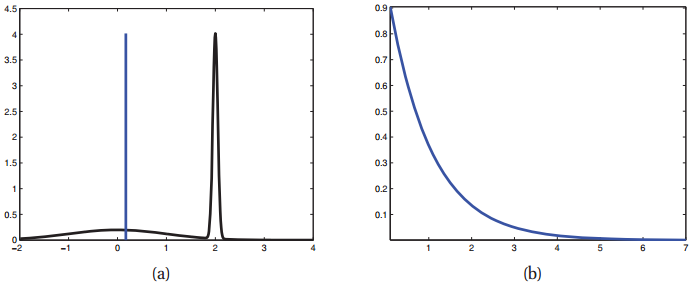
\includegraphics[scale=.70]{untypical-point.png}
\caption{(a) A bimodal distribution in which the mode is very untypical of the distribution. The thin blue vertical line is the mean, which is arguably a better summary of the distribution, since it is near the majority of the probability mass. (b) A skewed distribution in which the mode is quite different from the mean.}
\label{fig:untypical-point} 
\end{figure}

How should we summarize a posterior if the mode is not a good choice? The answer is to use decision theory, which we discuss in Section ~\ref{sec:Bayesian-decision-theory}. The basic idea is to specify a loss function, where $L(\theta,\hat{\theta})$ is the loss you incur if the truth is $\theta$ and your estimate is $\hat{\theta}$. If we use 0-1 loss $L(\theta,\hat{\theta})=\mathbb{I}(\theta \neq \hat{\theta})$(see section ~\ref{sec:Loss-function-and-risk-function}), then the optimal estimate is the posterior mode. 0-1 loss means you only get “points” if you make no errors, otherwise you get nothing: there is no “partial credit” under this loss function! For continuous-valued quantities, we often prefer to use squared error loss, $L(\theta,\hat{\theta})=(\theta-\hat{\theta})^2$ ; the corresponding optimal estimator is then the posterior mean, as we show in Section ~\ref{sec:Bayesian-decision-theory}. Or we can use a more robust loss function, $L(\theta,\hat{\theta})=|\theta-\hat{\theta}|$, which gives rise to the posterior median.

\subsubsection{MAP estimation is not invariant to reparameterization *}
A more subtle problem with MAP estimation is that the result we get depends on how we parameterize the probability distribution. Changing from one representation to another equivalent representation changes the result, which is not very desirable, since the units of measurement are arbitrary (e.g., when measuring distance, we can use centimetres or inches).

To understand the problem, suppose we compute the posterior forx. If we define y=f(x), the distribution for yis given by Equation ~\eqref{eqn:General-transformations}. The $\frac{\mathrm{d}x}{\mathrm{d}y}$ term is called the Jacobian, and it measures the change in size of a unit volume passed
through $f$. Let $\hat{x}=\arg\max_x p_x(x)$ be the MAP estimate for $x$. In general it is not the case that $\hat{x}=\arg\max_x p_x(x)$ is given by $f(\hat{x})$. For example, let $X \sim \mathcal{N}(6,1)$ and $y=f(x)$, where $f(x)=1/(1+\exp(-x+5))$. 

\begin{figure}[hbtp]
\centering
    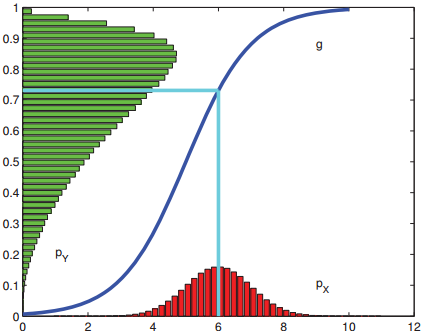
\includegraphics[scale=.70]{mode-reparameterization.png}
\caption{Example of the transformation of a density under a nonlinear transform. Note how the mode of the transformed distribution is not the transform of the original mode. Based on Exercise 1.4 of (Bishop 2006b).}
\label{fig:mode-reparameterization} 
\end{figure}

We can derive the distribution of $y$ using Monte Carlo simulation (see Section ~\ref{sec:Monte-Carlo-approximation}). The result is shown in Figure ~\ref{sec:mode-reparameterization}. We see that the original Gaussian has become “squashed” by the sigmoid nonlinearity. In particular, we see that the mode of the transformed distribution is not equal to the transform of the original mode.

The MLE does not suffer from this since the likelihood is a function, not a probability density. Bayesian inference does not suffer from this problem either, since the change of measure is taken into account when integrating over the parameter space.


\subsection{Credible intervals}
\label{sec:Credible-intervals}
In addition to point estimates, we often want a measure of confidence. A standard measure of confidence in some (scalar) quantity $\theta$ is the “width” of its posterior distribution. This can be measured using a $100(1−\alpha)\%$ credible interval, which is a (contiguous) region $C=(\ell,u)$(standing for lower and upper) which contains $1−\alpha$ of the posterior probability mass, i.e.,
\begin{equation}
C_{\alpha}(\mathcal{D}) \quad \text{where } P(\ell \leq \theta \leq u)=1-\alpha
\end{equation}

There may be many such intervals, so we choose one such that there is $(1−\alpha)/2$ mass in each tail; this is called a \textbf{central interval}.

If the posterior has a known functional form, we can compute the posterior central interval using $\ell=F^{-1}(\alpha/2)$ and $u=F^{-1}(1-\alpha/2)$, where $F$ is the cdf of the posterior. 

If we don’t know the functional form, but we can draw samples from the posterior, then we can use a Monte Carlo approximation to the posterior quantiles: we simply sort the $\mathcal{S}$ samples, and find the one that occurs at location $\alpha/\mathcal{S}$ along the sorted list. As $\mathcal{S} \rightarrow \infty$, this converges to the true quantile. 

People often confuse Bayesian credible intervals with frequentist confidence intervals. However, they are not the same thing, as we discuss in Section TODO. In general, credible intervals are usually what people want to compute, but confidence intervals are usually what they actually compute, because most people are taught frequentist statistics but not Bayesian statistics. Fortunately, the mechanics of computing a credible interval is just as easy as computing a confidence interval. 


\subsection{Inference for a difference in proportions}
Sometimes we have multiple parameters, and we are interested in computing the posterior distribution of some function of these parameters. For example, suppose you are about to buy something from Amazon.com, and there are two sellers offering it for the same price. Seller 1 has 90 positive reviews and 10 negative reviews. Seller 2 has 2 positive reviews and 0 negative reviews. Who should you buy from?\footnote{This example is from \url{http://www.johndcook.com/blog/2011/09/27/bayesian-amazon/}}.

On the face of it, you should pick seller 2, but we cannot be very confident that seller 2 is better since it has had so few reviews. In this section, we sketch a Bayesian analysis of this problem. Similar methodology can be used to compare rates or proportions across groups for a variety of other settings.

Let $\theta_1$ and $\theta_2$ be the unknown reliabilities of the two sellers. Since we don’t know much about them, we’ll endow them both with uniform priors, $\theta_i \sim \text{Beta}(1,1)$. The posteriors are $p(\theta_1|\mathcal{D}_1)=\text{Beta}(91,11)$ and $p(\theta_2|\mathcal{D}_2)=\text{Beta}(3,1)$.

We want to compute $p(\theta_1 >\theta_2|\mathcal{D})$. For convenience, let us define $\delta=\theta_1-\theta_2$ as the difference in the rates. (Alternatively we might want to work in terms of the log-odds ratio.) We can compute the desired quantity using numerical integration
\begin{equation}
p(\delta>0|\mathcal{D})=\int_0^1{\int_0^1{\mathbb{I}(\theta_1>\theta_2)\text{Beta}(\theta_1|91,11)\text{Beta}(\theta_2|3,1)}\mathrm{d}\theta_1}\mathrm{d}\theta_2
\end{equation}

We find $p(\delta>0|\mathcal{D})=0.710$, which means you are better off buying from seller 1! 


\section{Bayesian model selection}
In general, when faced with a set of models (i.e., families of parametric distributions) of different complexity, how should we choose the best one? This is called the \textbf{model selection} problem.

One approach is to use cross-validation to estimate the generalization error of all the candidate models, and then to pick the model that seems the best. However, this requires fitting each model $K$ times, where $K$ is the number of CV folds. A more efficient approach is to compute the posterior over models,
\begin{equation}
p(m|\mathcal{D})=\dfrac{p(\mathcal{D}|m)p(m)}{\sum_{m'}p(\mathcal{D}|m')p(m')}
\end{equation}

From this, we can easily compute the MAP model, $\hat{m}=\arg\max_m{p(m|\mathcal{D})}$. This is called \textbf{Bayesian model selection}.

If we use a uniform prior over models, this amounts to picking the model which maximizes
\begin{equation}\label{eqn:marginal-likelihood}
p(\mathcal{D}|m)=\int{p(\mathcal{D}|\vec{\theta})p(\vec{\theta}|m)}\mathrm{d}\vec{\theta}
\end{equation}

This quantity is called the \textbf{marginal likelihood}, the \textbf{integrated likelihood}, or the \textbf{evidence} for model $m$. The details on how to perform this integral will be discussed in Section ~\ref{sec:Computing-the-marginal-likelihood}. But first we give an intuitive interpretation of what this quantity means.


\subsection{Bayesian Occam's razor}
One might think that using $p(\mathcal{D}|m)$ to select models would always favour the model with the most parameters. This is true if we use $p(\mathcal{D}|\hat{\vec{\theta}}_m)$ to select models, where $\hat{\vec{\theta}}_m)$ is the MLE or MAP estimate of the parameters for model $m$, because models with more parameters will fit the data better, and hence achieve higher likelihood. However, if we integrate out the parameters, rather than maximizing them, we are automatically protected from overfitting: models with more parameters do not necessarily have higher \emph{marginal likelihood}. This is called the \textbf{Bayesian Occam’s razor} effect (MacKay 1995b; Murray and Ghahramani 2005), named after the principle known as \textbf{Occam’s razor}, which says one should pick the simplest model that adequately explains the data.

One way to understand the Bayesian Occam’s razor is to notice that the marginal likelihood can be rewritten as follows, based on the chain rule of probability (Equation ~\eqref{eqn:product-rule}):
\begin{equation}
p(D)=p((\vec{x}_1,y_1))p((\vec{x}_2,y_2)|(\vec{x}_1,y_1))p((\vec{x}_3,y_3)|(\vec{x}_1,y_1):(\vec{x}_2,y_2))\cdots p((\vec{x}_N,y_N)|(\vec{x}_1,y_1):(\vec{x}_{N-1},y_{N-1}))
\end{equation}

This is similar to a leave-one-out cross-validation estimate (Section ~\ref{sec:Cross-validation}) of the likelihood, since we predict each future point given all the previous ones. (Of course, the order of the data does not matter in the above expression.) If a model is too complex, it will overfit the “early” examples and will then predict the remaining ones poorly.

Another way to understand the Bayesian Occam’s razor effect is to note that probabilities must sum to one. Hence $\sum_{p(\mathcal{D}')} p(m|\mathcal{D}')=1$, where the sum is over all possible data sets. Complex models, which can predict many things, must spread their probability mass thinly, and hence will not obtain as large a probability for any given data set as simpler models. This is sometimes called the \textbf{conservation of probability mass} principle, and is illustrated in Figure ~\ref{fig:Bayesian-Occams-razor}.

\begin{figure}[hbtp]
\centering
    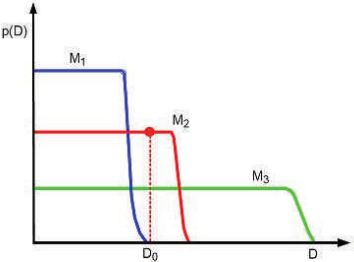
\includegraphics[scale=.80]{Bayesian-Occams-razor.png}
\caption{A schematic illustration of the Bayesian Occam’s razor. The broad (green) curve corresponds to a complex model, the narrow (blue) curve to a simple model, and the middle (red) curve is just right. Based on Figure 3.13 of (Bishop 2006a). }
\label{fig:Bayesian-Occams-razor} 
\end{figure}

When using the Bayesian approach, we are not restricted to evaluating the evidence at a finite grid of values. Instead, we can use numerical optimization to find $\lambda^*=\arg\max_{\lambda}p(\mathcal{D}|\lambda)$. This technique is called \textbf{empirical Bayes} or \textbf{type II maximum likelihood} (see Section ~\ref{sec:Empirical-Bayes} for details). An example is shown in Figure TODO(b): we see that the curve has a similar shape to the CV estimate, but it can be computed more efficiently.


\subsection{Computing the marginal likelihood (evidence)}
\label{sec:Computing-the-marginal-likelihood}
When discussing parameter inference for a fixed model, we often wrote
\begin{equation}
p(\vec{\theta}|\mathcal{D},m) \propto p(\vec{\theta}|m)p(\mathcal{D}|\vec{\theta},m)
\end{equation}
thus ignoring the normalization constant $p(\mathcal{D}|m)$. This is valid since $p(\mathcal{D}|m)$is constant wrt $\vec{\theta}$. However, when comparing models, we need to know how to compute the marginal likelihood, $p(\mathcal{D}|m)$. In general, this can be quite hard, since we have to integrate over all possible parameter values, but when we have a conjugate prior, it is easy to compute, as we now show.

Let $p(\vec{\theta})=q(\vec{\theta})/Z_0$ be our prior, where $q(\vec{\theta})$ is an unnormalized distribution, and $Z_0$ is the normalization constant of the prior. Let $p(\mathcal{D}|\vec{\theta})=q(\mathcal{D}|\vec{\theta})/Z_{\ell}$ be the likelihood, where $Z_{\ell}$ contains any constant factors in the likelihood. Finally let $p(\vec{\theta}|\mathcal{D})=q(\vec{\theta}|\mathcal{D})/Z_N$ be our posterior , where $q(\vec{\theta}|\mathcal{D})=q(\mathcal{D}|\vec{\theta})q(\vec{\theta})$ is the unnormalized posterior, and $Z_N$ is the normalization constant of the posterior. We have
\begin{align}
p(\vec{\theta}|\mathcal{D})& =\dfrac{p(\mathcal{D}|\vec{\theta})p(\vec{\theta})}{p(\mathcal{D})} \\
\dfrac{q(\vec{\theta}|\mathcal{D})}{Z_N}& =\dfrac{q(\mathcal{D}|\vec{\theta})q(\vec{\theta})}{Z_{\ell}Z_0p(\mathcal{D})} \\
p(\mathcal{D})& = \dfrac{Z_N}{Z_0Z_{\ell}}
\end{align}

So assuming the relevant normalization constants are tractable, we have an easy way to compute the marginal likelihood. We give some examples below.

\subsubsection{Beta-binomial model}
Let us apply the above result to the Beta-binomial model. Since we know $p(\vec{\theta}|\mathcal{D})=\mathrm{Beta}(\vec{\theta}|a',b')$, where $a'=a+N_1$, $b'=b+N_0$, we know the normalization constant of the posterior is $B(a',b')$. Hence
\begin{align}
p(\theta|\mathcal{D})& =\dfrac{p(\mathcal{D}|\theta)p(\theta)}{p(\mathcal{D})} \\
    & =\dfrac{1}{p(\mathcal{D})}\left[\dfrac{1}{B(a,b)}\theta^{a-1}(1-\theta)^{b-1}\right]\left[\dbinom{N}{N_1}\theta^{N_1}(1-\theta)^{N_0}\right] \\
	& =\dbinom{N}{N_1}\dfrac{1}{p(\mathcal{D})}\dfrac{1}{B(a,b)}\left[\theta^{a+N_1-1}(1-\theta)^{b+N_0-1}\right]
\end{align}

So
\begin{align}
\dfrac{1}{B(a+N_1,b+N_0)} & = \dbinom{N}{N_1}\dfrac{1}{p(\mathcal{D})}\dfrac{1}{B(a,b)} \\
p(\mathcal{D}) & = \dbinom{N}{N_1}\dfrac{B(a+N_1,b+N_0)}{B(a,b)}
\end{align}

The marginal likelihood for the Beta-Bernoulli model is the same as above, except it is missingthe $\binom{N}{N_1}$ term.

\subsubsection{Dirichlet-multinoulli model}
By the same reasoning as the Beta-Bernoulli case, one can show that the marginal likelihood for the Dirichlet-multinoulli model is given by
\begin{align}
p(\mathcal{D}) & =\dfrac{B(\vec{N}+\vec{\alpha})}{B(\vec{\alpha})} \\
   & = \dfrac{\Gamma(\sum_k \alpha_k)}{\Gamma(N+\sum_k \alpha_k)}\prod\limits_k \dfrac{\Gamma(N_k+\alpha_k)}{\Gamma(\alpha_k)}
\end{align}

\subsubsection{Gaussian-Gaussian-Wishart model}
Consider the case of an MVN with a conjugate NIW prior. Let $Z_0$ be the normalizer for the prior, $Z_N$ be normalizer for the posterior, and let $Z_{\ell}(2\pi)^{ND/2}=$ be the normalizer for the likelihood. Then it is easy to see that
\begin{align}
p(\mathcal{D})& =\dfrac{Z_N}{Z_0Z_{\ell}} \\
   & = \dfrac{1}{\pi^{ND/2}}\dfrac{1}{2^{ND/2}}\dfrac{\left(\frac{2\pi}{\kappa_N}\right)^{D/2}|\vec{S}_N|^{-\nu_N/2}2^{(\nu_0+N)D/2}\Gamma_D(\nu_N/2)}{\left(\frac{2\pi}{\kappa_0}\right)^{D/2}|\vec{S}_0|^{-\nu_0/2}2^{\nu_0D/2}\Gamma_D(\nu_0/2)} \\
   & \dfrac{1}{\pi^{ND/2}}\left(\dfrac{\kappa_0}{\kappa_N}\right)^{D/2}\dfrac{|\vec{S}_0|^{\nu_0/2}}{|\vec{S}_N|^{\nu_N/2}}\dfrac{\Gamma_D(\nu_N/2)}{\Gamma_D(\nu_0/2)}
\end{align}

\subsubsection{BIC approximation to log marginal likelihood}
In general, computing the integral in Equation ~\eqref{eqn:marginal-likelihood} can be quite difficult. One simple but popular approximation is known as the \textbf{Bayesian information criterion} or \textbf{BIC}, which has the following form (Schwarz 1978):
\begin{equation}
\mathrm{BIC} \triangleq \log p(\mathcal{D}|\hat{\vec{\theta}})-\dfrac{\mathrm{dof}(\hat{\vec{\theta}})}{2}\log{N}
\end{equation}
where $\mathrm{dof}(\hat{\vec{\theta}})$ is the number of \textbf{degrees of freedom} in the model, and $\hat{\vec{\theta}}$ is the MLE for the model. We see that this has the form of a \textbf{penalized log likelihood}, where the penalty term depends on the model’s complexity. See Section TODO for the derivation of the BIC score.

As an example, consider linear regression. As we show in Section TODO, the MLE is given by $\hat{\vec{w}}=(\vec{X}^T\vec{X})^{-1}\vec{X}^T\vec{y}$ and $\sigma^2=\frac{1}{N}\sum_{i=1}^N (y_i-\hat{\vec{w}}^T\vec{x}_i)$. The corresponding log likelihood is given by
\begin{equation}
\log p(\mathcal{D}|\hat{\vec{\theta}}) = -\dfrac{N}{2}\log(2\pi\hat{\sigma}^2)-\dfrac{N}{2}
\end{equation}

Hence the BIC score is as follows (dropping constant terms)
\begin{equation}
\mathrm{BIC}=-\dfrac{N}{2}\log(\hat{\sigma}^2)-\dfrac{D}{2}\log{N}
\end{equation}
where $D$ is the number of variables in the model. In the statistics literature, it is common to use an alternative definition of BIC, which we call the BIC \emph{cost}(since we want to minimize it):
\begin{equation}
\mathrm{BIC\text{-}cost} \triangleq -2\log p(\mathcal{D}|\hat{\vec{\theta}})-\mathrm{dof}(\hat{\vec{\theta}})\log{N} \approx -2\log{p(\mathcal{D})}
\end{equation}

In the context of linear regression, this becomes
\begin{equation}
\mathrm{BIC\text{-}cost} = N\log(\hat{\sigma}^2)+D\log{N}
\end{equation}

The BIC method is very closely related to the \textbf{minimum description length} or \textbf{MDL} principle, which characterizes the score for a model in terms of how well it fits the data, minus how complex the model is to define. See (Hansen and Yu 2001) for details.

There is a very similar expression to BIC/ MDL called the \textbf{Akaike information criterion} or \textbf{AIC}, defined as
\begin{equation}
\mathrm{AIC}(m,\mathcal{D}) = \log{p(\mathcal{D}|\hat{\vec{\theta}}_{MLE})}-\mathrm{dof}(m)
\end{equation}

This is derived from a frequentist framework, and cannot be interpreted as an approximation to the marginal likelihood. Nevertheless, the form of this expression is very similar to BIC. We see that the penalty for AIC is less than for BIC. This causes AIC to pick more complex models. However, this can result in better predictive accuracy. See e.g., (Clarke et al. 2009, sec 10.2) for further discussion on such information criteria.

\subsubsection{Effect of the prior}
Sometimes it is not clear how to set the prior. When we are performing posterior inference, the details of the prior may not matter too much, since the likelihood often overwhelms the prior anyway. But when computing the marginal likelihood, the prior plays a much more important role, since we are averaging the likelihood over all possible parameter settings, as weighted by the prior.

If the prior is unknown, the correct Bayesian procedure is to put a prior on the prior. If the prior is unknown, the correct Bayesian procedure is to put a prior on the prior. 


\subsection{Bayes factors}
Suppose our prior on models is uniform, $p(m) \propto 1$. Then model selection is equivalent to picking the model with the highest marginal likelihood. Now suppose we just have two models we are considering, call them the \textbf{null hypothesis}, $M_0$, and the \textbf{alternative hypothesis}, $M_1$. Define the \textbf{Bayes factor} as the ratio of marginal likelihoods:
\begin{equation}
\mathrm{BF}_{1,0} \triangleq \dfrac{p(\mathcal{D}|M_1)}{p(\mathcal{D}|M_0)}=\dfrac{p(M_1|\mathcal{D})}{p(M_2|\mathcal{D})}/\dfrac{p(M_1)}{p(M_0)}
\end{equation}


\section{Priors}
The most controversial aspect of Bayesian statistics is its reliance on priors. Bayesians argue this is unavoidable, since nobody is a \textbf{tabula rasa} or \textbf{blank slate}: all inference must be done conditional on certain assumptions about the world. Nevertheless, one might be interested in minimizing the impact of one’s prior assumptions. We briefly discuss some ways to do this below.


\subsection{Uninformative priors}
If we don’t have strong beliefs about what $\theta$ should be, it is common to use an \textbf{uninformative} or \textbf{non-informative} prior, and to “let the data speak for itself”.


\subsection{Robust priors}
In many cases, we are not very confident in our prior, so we want to make sure it does not have an undue influence on the result. This can be done by using \textbf{robust priors}(Insua and Ruggeri 2000), which typically have heavy tails, which avoids forcing things to be too close to the prior mean.


\subsection{Mixtures of conjugate priors}
Robust priors are useful, but can be computationally expensive to use. Conjugate priors simplify the computation, but are often not robust, and not flexible enough to encode our prior knowledge. However, it turns out that a \textbf{mixture of conjugate priors} is also conjugate, and can approximate any kind of prior (Dallal and Hall 1983; Diaconis and Ylvisaker 1985). Thus such priors provide a good compromise between computational convenience and flexibility.


\section{Hierarchical Bayes}
A key requirement for computing the posterior $p(\vec{\theta}|\mathcal{D})$ is the specification of a prior $p(\vec{\theta}|\vec{\eta})$, where $\vec{\eta}$ are the hyper-parameters. What if we don’t know how to set $\vec{\eta}$? In some cases, we can use uninformative priors, we we discussed above. A more Bayesian approach is to put a prior on our priors! In terms of graphical models (Chapter TODO), we can represent the situation as follows:
\begin{equation}
\vec{\eta} \rightarrow \vec{\theta} \rightarrow \mathcal{D}
\end{equation}

This is an example of a \textbf{hierarchical Bayesian model}, also called a \textbf{multi-level} model, since there are multiple levels of unknown quantities. 


\section{Empirical Bayes}
\label{sec:Empirical-Bayes}
\begin{longtable}{ll}
\hline\noalign{\smallskip}
\textbf{Method} & \textbf{Definition} \\
\noalign{\smallskip}\hline\noalign{\smallskip}
Maximum likelihood & $\hat{\vec{\theta}}=\arg\max_{\vec{\theta}} p(\mathcal{D}|\vec{\theta})$ \\
MAP estimation & $\hat{\vec{\theta}}=\arg\max_{\vec{\theta}} p(\mathcal{D}|\vec{\theta})p(\vec{\theta}|\vec{\eta})$ \\
ML-II (\textbf{Empirical Bayes}) & $\hat{\vec{\eta}}=\arg\max_{\vec{\eta}} \int p(\mathcal{D}|\vec{\theta})p(\vec{\theta}|\vec{\eta})\mathrm{d}\vec{\theta}=\arg\max_{\vec{\eta}}p(\mathcal{D}|\vec{\eta})$ \\
MAP-II & $\hat{\vec{\eta}}=\arg\max_{\vec{\eta}} \int p(\mathcal{D}|\vec{\theta})p(\vec{\theta}|\vec{\eta})p(\vec{\eta})\mathrm{d}\vec{\theta}=\arg\max_{\vec{\eta}}p(\mathcal{D}|\vec{\eta})p(\vec{\eta})$ \\
Full Bayes & $p(\vec{\theta},\vec{\eta}|\mathcal{D}) \propto p(\mathcal{D}|\vec{\theta})p(\vec{\theta}|\vec{\eta})$ \\
\noalign{\smallskip}\hline\noalign{\smallskip}
\end{longtable}


\section{Bayesian decision theory}
\label{sec:Bayesian-decision-theory}
We have seen how probability theory can be used to represent and updates our beliefs about the state of the world. However, ultimately our goal is to convert our beliefs into actions. In this section, we discuss the optimal way to do this.

Our goal is to devise a \textbf{decision procedure} or \textbf{policy}, $f(\vec{x}) : \mathcal{X} \rightarrow \mathcal{Y}$, which minimizes the \textbf{expected loss} $R_{\mathrm{exp}}(f)$(see Equation ~\eqref{eqn:expected-loss}).

In the Bayesian approach to decision theory, the optimal output, having observed $\vec{x}$, is defined as the output $a$ that minimizes the \textbf{posterior expected loss}:
\begin{equation}
\rho(f)=\mathbb{E}_{p(y|\vec{x})}[L(y,f(\vec{x}))]=\begin{cases}
\sum\limits_y L[y,f(\vec{x})]p(y|\vec{x}) & \text{, $y$ is discrete}\\
\int\limits_y L[y,f(\vec{x})]p(y|\vec{x})\mathrm{d}y & \text{, $y$ is continuous}
\end{cases}
\end{equation}

Hence the \textbf{Bayes estimator}, also called the \textbf{Bayes decision rule}, is given by
\begin{equation}
\delta(\vec{x})=\arg\min\limits_{f \in \mathcal{H}} \rho(f)
\end{equation}


\subsection{Bayes estimators for common loss functions}


\subsubsection{MAP estimate minimizes 0-1 loss}
When $L(y,f(x))$ is \textbf{0-1 loss}(Section ~\ref{sec:Loss-function-and-risk-function}), we can proof that MAP estimate minimizes 0-1 loss, 
\begin{align*}
\arg\min\limits_{f \in \mathcal{H}} \rho(f)& =\arg\min\limits_{f \in \mathcal{H}} \sum\limits_{i=1}^K{L[C_k,f(\vec{x})]p(C_k|\vec{x})} \\
         & =\arg\min\limits_{f \in \mathcal{H}} \sum\limits_{i=1}^K{\mathbb{I}(f(\vec{x}) \neq C_k)p(C_k|\vec{x})} \\
		 & =\arg\min\limits_{f \in \mathcal{H}} \sum\limits_{i=1}^K{p(f(\vec{x}) \neq C_k|\vec{x})} \\
		 & =\arg\min\limits_{f \in \mathcal{H}} \left[1-{p(f(\vec{x}) = C_k|\vec{x})}\right] \\
		 & =\arg\max\limits_{f \in \mathcal{H}} p(f(\vec{x}) = C_k|\vec{x})
\end{align*}


\subsubsection{Posterior mean minimizes	$\ell_2$(quadratic) loss}
For continuous parameters, a more appropriate loss function is \textbf{squared error}, \textbf{$\ell_2$ loss}, or \textbf{quadratic loss}, defined as $L(y,f(\vec{x}))=\left[y-f(\vec{x})\right]^2$.

The posterior expected loss is given by
\begin{equation}
\rho(f)=\int\limits_y L[y,f(\vec{x})]p(y|\vec{x})\mathrm{d}y=\int\limits_y \left[y-f(\vec{x})\right]^2p(y|\vec{x})\mathrm{d}y=\int\limits_y \left[y^2-2yf(\vec{x})+f(\vec{x})^2\right]p(y|\vec{x})\mathrm{d}y
\end{equation}

Hence the optimal estimate is the posterior mean:
\begin{align}
& \dfrac{\partial \rho}{\partial f} =\int\limits_y [-2y+2f(\vec{x})]p(y|\vec{x})\mathrm{d}y=0 \Rightarrow \nonumber \\
& \int\limits_y f(\vec{x})p(y|\vec{x})\mathrm{d}y = \int\limits_y yp(y|\vec{x})\mathrm{d}y \nonumber \\
& f(\vec{x}) \int\limits_y p(y|\vec{x})\mathrm{d}y = \mathbb{E}_{p(y|\vec{x})}[y] \nonumber \\
& f(\vec{x}) = \mathbb{E}_{p(y|\vec{x})}[y]
\end{align}

This is often called the \textbf{minimum mean squared error} estimate or \textbf{MMSE} estimate.


\subsubsection{Posterior median minimizes $\ell_1$(absolute) loss}
The $\ell_2$ loss penalizes deviations from the truth quadratically, and thus is sensitive to outliers. A more robust alternative is the absolute or $\ell_1$ loss. The optimal estimate is the posterior median, i.e., a value $a$ such that $P(y<a|\vec{x})=P(y \geq a|\vec{x})=0.5$.

\begin{proof}
TODO
\end{proof}


\subsubsection{Reject option}
In classification problems where $p(y|\vec{x})$ is very uncertain, we may prefer to choose a reject action, in which we refuse to classify the example as any of the specified classes, and instead say “don’t know”. Such ambiguous cases can be handled by e.g., a human expert. This is useful in \textbf{risk averse} domains such as medicine and finance.

We can formalize the reject option as follows. Let choosing $f(\vec{x})=c_{K+1}$ correspond to picking the reject action, and choosing $f(\vec{x}) \in \{C_1,...,C_k\}$ correspond to picking one of the classes. Suppose we define the loss function as
\begin{equation}
L(f(\vec{x}), y)=\begin{cases} 
0 & \text{if } f(\vec{x})=y \text{ and } f(\vec{x}),y \in \{C_1,...,C_k\} \\
\lambda_s & \text{if } f(\vec{x}) \neq y \text{ and } f(\vec{x}),y \in \{C_1,...,C_k\} \\
\lambda_r & \text{if } f(\vec{x})=C_{K+1}
\end{cases}
\end{equation}
where $\lambda_s$ is the cost of a substitution error, and $\lambda_r$ is the cost of the reject action. 


\subsubsection{Supervised learning}
We can define the loss incurred by $f(\vec{x})$ (i.e., using this predictor) when the unknown state of nature is $\vec{\theta}$(the parameters of the data generating mechanism) as follows:
\begin{equation}
L(\vec{\theta},f) \triangleq \mathbb{E}_{p(\vec{x},y|\vec{\theta})}[\ell(y-f(\vec{x}))]
\end{equation}

This is known as the \textbf{generalization error}. Our goal is to minimize the posterior expected loss, given by
\begin{equation}
\rho(f|\mathcal{D}) = \int{p(\vec{\theta}|\mathcal{D})L(\vec{\theta},f)}\mathrm{d}\vec{\theta}
\end{equation}

This should be contrasted with the frequentist risk which is defined in Equation TODO.


\subsection{The false positive vs false negative tradeoff}
In this section, we focus on binary decision problems, such as hypothesis testing, two-class classification, object/ event detection, etc. There are two types of error we can make: a \textbf{false positive}(aka \textbf{false alarm}), or a \textbf{false negative}(aka \textbf{missed detection}). The 0-1 loss treats these two kinds of errors equivalently. However, we can consider the following more general loss matrix:

TODO

\chapter{Frequentist statistics}

Attempts have been made to devise approaches to statistical inference that avoid treating parameters like random variables, and which thus avoid the use of priors and Bayes rule. Such approaches are known as \textbf{frequentist statistics}, \textbf{classical statistics} or \textbf{orthodox statistics}. Instead of being based on the posterior distribution, they are based on the concept of a sampling distribution.


\section{Sampling distribution of an estimator}
In frequentist statistics, a parameter estimate $\hat{\vec{\theta}}$ is computed by applying an \textbf{estimator} $\delta$ to some data $\mathcal{D}$, so $\hat{\vec{\theta}}=\delta(\mathcal{D})$. The parameter is viewed as fixed and the data as random, which is the exact opposite of the Bayesian approach. The uncertainty in the parameter estimate can be measured by computing the \textbf{sampling distribution} of the estimator. To understand this


\subsection{Bootstrap}
We might think of the bootstrap distribution as a “poor man’s” Bayes posterior, see (Hastie et al. 2001, p235) for details.


\subsection{Large sample theory for the MLE *}



\section{Frequentist decision theory}
In frequentist or classical decision theory, there is a loss function and a likelihood, but there is no prior and hence no posterior or posterior expected loss. Thus there is no automatic way of deriving an optimal estimator, unlike the Bayesian case. Instead, in the frequentist approach, we are free to choose any estimator or decision procedure $f: \mathcal{X} \rightarrow \mathcal{Y}$ we want.

Having chosen an estimator, we define its expected loss or \textbf{risk} as follows:
\begin{equation}
R_{\mathrm{exp}}(\theta,f) \triangleq \mathbb{E}_{p(\tilde{\mathcal{D}}|\theta^*)}[L(\theta^*, f(\tilde{\mathcal{D}}))]=\int L(\theta^*, f(\tilde{\mathcal{D}}))p(\tilde{\mathcal{D}}|\theta^*)\mathrm{d}\tilde{\mathcal{D}}
\end{equation}
where˜$\tilde{\mathcal{D}}$ is data sampled from “nature’s distribution”, which is represented by parameter $\theta^*$. In other words, the expectation is wrt the sampling distribution of the estimator. Compare this to the Bayesian posterior expected loss:
\begin{equation}
\rho(f|\mathcal{D},)
\end{equation}


\section{Desirable properties of estimators}


\section{Empirical risk minimization}


\subsection{Regularized risk minimization}


\subsection{Structural risk minimization}


\subsection{Estimating the risk using cross validation}


\subsection{Upper bounding the risk using statistical learning theory *}


\subsection{Surrogate loss functions}
\label{sec:Surrogate-loss-functions}

\textbf{log-loss}
\begin{equation}\label{eqn:log-loss}
L_{\mathrm{nll}}(y,\eta)=-\log p(y|\vec{x},\vec{w})=\log(1+e^{-y\eta})
\end{equation}


\section{Pathologies of frequentist statistics *}


\chapter{Linear Regression}


\section{Introduction}
Linear regression is the “work horse” of statistics and (supervised) machine learning. When augmented with kernels or other forms of basis function expansion, it can model also nonlinear relationships. And when the Gaussian output is replaced with a Bernoulli or multinoulli distribution, it can be used for classification, as we will see below. So it pays to study this model in detail.


\section{Representation}
Linear regression is a model of the form
\begin{equation}
p(y|\vec{x},\vec{\theta})=\mathcal{N}(y|\vec{w}^T\vec{x}, \sigma^2)
\end{equation}
where $\vec{w}$ and $\vec{x}$ are extended vectors, $\vec{x}=(1,x)$, $\vec{w}=(b,w)$.

Linear regression can be made to model non-linear relationships by replacing $\vec{x}$ with some non-linear function of the inputs, $\phi(\vec{x})$ \begin{equation}
p(y|\vec{x},\vec{\theta})=\mathcal{N}(y|\vec{w}^T\phi(\vec{x}), \sigma^2)
\end{equation}

This is known as \textbf{basis function expansion}. (Note that the model is still linear in the parameters $\vec{w}$, so it is still called linear regression; the importance of this will become clear below.) A simple example are polynomial basis functions, where the model has the form
\begin{equation}
\phi(x)=(1, x, \cdots, x^d)
\end{equation}



\section{MLE}
Instead of maximizing the log-likelihood, we can equivalently minimize the \textbf{negative log likelihood} or \textbf{NLL}:
\begin{equation}
\text{NLL}(\vec{\theta}) \triangleq -\ell(\vec{\theta})=-\log(\mathcal{D}|\vec{\theta})
\end{equation}

The NLL formulation is sometimes more convenient, since many optimization software packages are designed to find the minima of functions, rather than maxima.

Now let us apply the method of MLE to the linear regression setting. Inserting the definition of the Gaussian into the above, we find that the log likelihood is given by
\begin{align}
\ell(\vec{\theta})& =\sum\limits_{i=1}^N \log\left[\dfrac{1}{\sqrt{2\pi}\sigma}\exp\left(-\dfrac{1}{2\sigma^2}(y_i-\vec{w}^T\vec{x}_i)^2\right)\right] \\
     & =-\dfrac{1}{2\sigma^2}\text{RSS}(\vec{w})-\dfrac{\vec{w}}{2}\log(2\pi\sigma^2)
\end{align}

RSS stands for \textbf{residual sum of squares} and is defined by
\begin{equation}
\text{RSS}(\vec{w}) \triangleq \sum\limits_{i=1}^N (y_i-\vec{w}^T\vec{x}_i)^2
\end{equation}

We see that the MLE for $\vec{w}$ is the one that minimizes the RSS, so this method is known as \textbf{least squares}.

Let's drop constants wrt $\vec{w}$ and NLL can be written as
\begin{equation}
\text{NLL}(\vec{w}) = \dfrac{1}{2}\sum\limits_{i=1}^N (y_i-\vec{w}^T\vec{x}_i)^2
\end{equation}

There two ways to minimize NLL$(\vec{w})$.


\subsection{OLS}
Define $\vec{y}=(y_1,y_2,\cdots,y_N)$, $\vec{X}=\left(\begin{array}{c}\vec{x}_1^T \\ \vec{x}_2^T \\ \vdots \\ \vec{x}_N^T\end{array}\right)$, then NLL$(\vec{w})$ can be written as
\begin{equation}
\text{NLL}(\vec{w})=\dfrac{1}{2}(\vec{y}-\vec{X}\vec{w})^T(\vec{y}-\vec{X}\vec{w})
\end{equation}

When $\mathcal{D}$ is small(for example, $N < 1000$), we can use the following equation to compute \vec{w} directly
\begin{equation}
\hat{\vec{w}}_{\mathrm{OLS}}=(\vec{X}^T\vec{X})^{-1}\vec{X}^T\vec{y}
\end{equation}

The corresponding solution $\hat{\vec{w}}_{\mathrm{OLS}}$ to this linear system of equations is called the \textbf{ordinary least squares} or \textbf{OLS} solution.

\begin{proof}
We now state without proof some facts of matrix derivatives (we won’t need all of these at this section).
\begin{eqnarray}
trA &\triangleq& \sum\limits_{i=1}^n A_{ii} \nonumber \\
\frac{\partial}{\partial A}AB &=& B^T \\
\frac{\partial}{\partial A^T}f(A) &=& \left[\frac{\partial}{\partial A}f(A)\right]^T \label{eqn:matrix-1} \\
\frac{\partial}{\partial A}ABA^TC &=& CAB+C^TAB^T \label{eqn:matrix-2} \\
\frac{\partial}{\partial A}|A| &=& |A|(A^{-1})^T
\end{eqnarray}

Then,
\begin{eqnarray*}
\text{NLL}(\vec{w}) &=& \frac{1}{2N}(\vec{X}\vec{w}-\vec{y})^T(\vec{X}\vec{w}-\vec{y}) \\
\frac{\partial \text{NLL}}{\vec{w}} &=& \frac{1}{2} \frac{\partial}{\vec{w}} (\vec{w}^T\vec{X}^T\vec{X}\vec{w}-\vec{w}^T\vec{X}^T\vec{y}-\vec{y}^T\vec{X}\vec{w}+\vec{y}^T\vec{y}) \\
                           &=& \frac{1}{2} \frac{\partial}{\vec{w}} (\vec{w}^T\vec{X}^T\vec{X}\vec{w}-\vec{w}^T\vec{X}^T\vec{y}-\vec{y}^T\vec{X}\vec{w}) \\
						   &=& \frac{1}{2} \frac{\partial}{\vec{w}} tr(\vec{w}^T\vec{X}^T\vec{X}\vec{w}-\vec{w}^T\vec{X}^T\vec{y}-\vec{y}^T\vec{X}\vec{w}) \\
						   &=& \frac{1}{2} \frac{\partial}{\vec{w}} (tr\vec{w}^T\vec{X}^T\vec{X}\vec{w}-2tr\vec{y}^T\vec{X}\vec{w})
\end{eqnarray*}

Combining Equations \eqref{eqn:matrix-1} and \eqref{eqn:matrix-2}, we find that 
\begin{equation*}
\frac{\partial}{\partial A^T}ABA^TC = B^TA^TC^T+BA^TC
\end{equation*}

Let $A^T=\vec{w}, B=B^T=\vec{X}^T\vec{X}$, and $C=I$, Hence,
\begin{eqnarray}
\frac{\partial \text{NLL}}{\vec{w}} &=& \frac{1}{2} (\vec{X}^T\vec{X}\vec{w}+\vec{X}^T\vec{X}\vec{w} -2\vec{X}^T\vec{y}) \nonumber \\
						   &=& \frac{1}{2} (\vec{X}^T\vec{X}\vec{w} - \vec{X}^T\vec{y}) \nonumber \\
\frac{\partial \text{NLL}}{\vec{w}} &=& 0 \Rightarrow \vec{X}^T\vec{X}\vec{w} - \vec{X}^T\vec{y} =0 \nonumber \\
\vec{X}^T\vec{X}\vec{w} &=& \vec{X}^T\vec{y} \label{eqn:normal-equation} \\
\hat{\vec{w}}_{\mathrm{OLS}} &=& (\vec{X}^T\vec{X})^{-1}\vec{X}^T\vec{y} \nonumber
\end{eqnarray}
\end{proof}

Equation \eqref{eqn:normal-equation} is known as the \textbf{normal equation}.


\subsubsection{Geometric interpretation}

See Figure \ref{fig:graphical-interpretation-of-OLS}.
\begin{figure}[hbtp]
\centering
    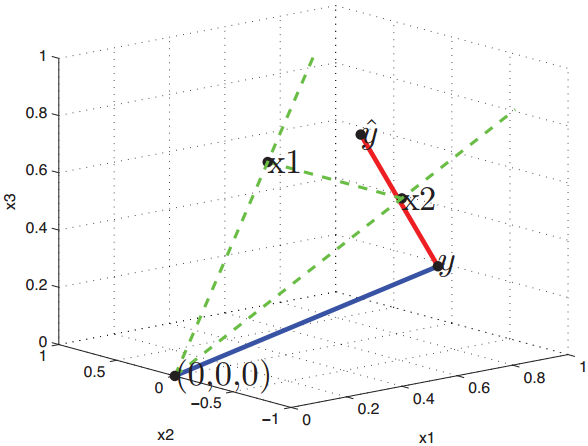
\includegraphics[scale=.60]{graphical-interpretation-of-OLS.png}
\caption{Graphical interpretation of least squares for $N=3$ examples and $D=2$ features. $\tilde{\vec{x}}_1$ and $\tilde{\vec{x}}_2$˜ are vectors in $\mathbb{R}^3$; together they define a 2D plane. $\vec{y}$ is also a vector in $\mathbb{R}^3$ but does not lie on this 2D plane. The orthogonal projection of $\vec{y}$ onto this plane is denoted $\hat{\vec{y}}$. The red line from $\vec{y}$ to $\hat{\vec{y}}$ is the residual, whose norm we want to minimize. For visual clarity, all vectors have been converted to unit norm.}
\label{fig:graphical-interpretation-of-OLS} 
\end{figure}

To minimize the norm of the residual, $\vec{y}-\hat{\vec{y}}$, we want the residual vector to be orthogonal to every column of $\vec{X}$,so˜ $\tilde{\vec{x}}_j(\vec{y}-\hat{\vec{y}})=0$ for $j=1:D$. Hence
\begin{equation}
\tilde{\vec{x}}_j(\vec{y}-\hat{\vec{y}})=0 \Rightarrow \vec{X}^T(\vec{y}-\vec{X}\vec{w})=0 \Rightarrow \vec{w}=(\vec{X}^T\vec{X})^{-1}\vec{X}^T\vec{y}
\end{equation}


\subsection{SGD}
When $\mathcal{D}$ is large, use stochastic gradient descent(SGD).

\begin{align}
\because \dfrac{\partial}{\partial w_i}\text{NLL}(\vec{w})=& \sum\limits_{i=1}^N (\vec{w}^T\vec{x}_i-y_i)x_{ij} \\
\therefore w_j=& w_j - \alpha\dfrac{\partial}{\partial w_j}\text{NLL}(\vec{w}) \nonumber \\
                  =& w_j - \sum\limits_{i=1}^N \alpha(\vec{w}^T\vec{x}_i-y_i)x_{ij} \\
\therefore \vec{w}=& \vec{w}-\alpha(\vec{w}^T\vec{x}_i-y_i)\vec{x}
\end{align}


\section{Ridge regression(MAP)}
One problem with ML estimation is that it can result in overfitting. In this section, we discuss a way to ameliorate this problem by using MAP estimation with a Gaussian prior.


\subsection{Basic idea}
We can encourage the parameters to be small, thus resulting in a smoother curve, by using a zero-mean Gaussian prior:
\begin{equation}
p(\vec{w})=\prod\limits_j \mathcal{N}(w_j|0,\tau^2)
\end{equation}
where $1/\tau^2$ controls the strength of the prior. The corresponding MAP estimation problem becomes
\begin{equation}
\arg\max_{\vec{w}} \sum\limits_{i=1}^N \log{\mathcal{N}(y_i|w_0+\vec{w}^T\vec{x}_i,\sigma^2)}+\sum\limits_{j=1}^D \log{\mathcal{N}(w_j|0,\tau^2)}
\end{equation}

It is a simple exercise to show that this is equivalent to minimizing the following
\begin{equation}
J(\vec{w})=\dfrac{1}{N}\sum\limits_{i=1}^N (y_i-(w_0+\vec{w}^T\vec{x}_i))^2+\lambda\lVert\vec{w}\rVert^2 \quad \text{, where }\lambda \triangleq \dfrac{\sigma^2}{\tau^2}
\end{equation}

Here the first term is the MSE/ NLL as usual, and the second term, $\lambda \geq 0$, is a complexity penalty. The corresponding solution is given by
\begin{equation}
\hat{\vec{w}}_{\mathrm{ridge}}=(\lambda\vec{I}_D+\vec{X}^T\vec{X})^{-1}\vec{X}^T\vec{y}
\end{equation}

This technique is known as \textbf{ridge regression},or \textbf{penalized least squares}. In general, adding a Gaussian prior to the parameters of a model to encourage them to be small is called $\ell_2$ \textbf{regularization} or \textbf{weight decay}. Note that the offset term $w_0$ is not regularized, since this just affects the height of the function, not its complexity.

We will consider a variety of different priors in this book. Each of these corresponds to a different form of \textbf{regularization}. This technique is very widely used to prevent overfitting.


\subsection{Regularization effects of big data}
Regularization is the most common way to avoid overfitting. However, another effective approach — which is not always available — is to use lots of data. It should be intuitively obvious that the more training data we have, the better we will be able to learn.

In domains with lots of data, simple methods can work surprisingly well (Halevy et al. 2009). However, there are still reasons to study more sophisticated learning methods, because there will always be problems for which we have little data. For example, even in such a data-rich domain as web search, as soon as we want to start personalizing the results, the amount of data available for any given user starts to look small again (relative to the complexity of the problem).


\section{Bayesian linear regression}
TODO


\chapter{Logistic Regression}


\section{Binomial Logistic Regression Model}


\subsection{Representation}

\begin{eqnarray}
  P(Y=1|\vec{x}) &=& \frac{\exp(\vec{w}^T\vec{x})}{1+\exp(\vec{w}^T\vec{x})} \\
  P(Y=0|\vec{x}) &=& \frac{1}{1+\exp(\vec{w}^T\vec{x})}
\end{eqnarray}
where $\vec{w}=(w_1, w_2,\cdots, w_n, b)$, $\vec{x}=(x_1,x_2,\cdots, 1)$.


\subsection{Evaluation}
\begin{equation}
\max_{\vec{w}} \ell(\vec{w})
\end{equation}
where $\ell(\vec{w})$ is log likelihood function
\begin{eqnarray*}
\pi(\vec{x}_i) & \triangleq & P(Y=1|\vec{x}_i) \\
\ell(\vec{w}) &=& \log\left\{\prod\limits_{i=1}^N{\left[\pi(\vec{x}_i)\right]^{y_i}\left[1-\pi(\vec{x}_i)\right]^{1-y_i}}\right\} \\
           &=& \sum\limits_{i=1}^N\left[y_i\log\pi(\vec{x}_i)+(1-y_i)\log(1-\pi(\vec{x}_i))\right] \\
		   &=& \sum\limits_{i=1}^N\left[y_i\log\dfrac{\pi(\vec{x}_i)}{1-\pi(\vec{x}_i)}+\log(1-\pi(\vec{x}_i))\right] \\
		   &=& \sum\limits_{i=1}^N\left[y_i(\vec{w}\cdot\vec{x}_i)-\log(1+\exp(\vec{w}\cdot\vec{x}_i))\right]
\end{eqnarray*}


\subsection{Optimization}
We can use stochastic gradient ascent(SGA) and quasi Newton method, etc.


\subsubsection{SGA}
\begin{eqnarray}
\dfrac{\partial}{\partial \vec{w}}\ell(\vec{w}) &=& \left[y_i - \pi(\vec{x}_i) \right]\vec{x}_i \\
\vec{w} &=& \vec{w}+\alpha\dfrac{\partial}{\partial \vec{w}}\ell(\vec{w}) \nonumber \\
        &=& \vec{w} + \alpha\left[y_i - \pi(\vec{x}_i) \right]\vec{x}_i
\end{eqnarray}

\chapter{Generalized linear models and the exponential family}
\label{chap:GLM}


\section{The exponential family}
\label{sec:exponential-family}

Before defining the exponential family, we mention several reasons why it is important:
\begin{itemize}
\item{It can be shown that, under certain regularity conditions, the exponential family is the only family of distributions with finite-sized sufficient statistics, meaning that we can compress the data into a fixed-sized summary without loss of information. This is particularly useful for online learning, as we will see later.}
\item{The exponential family is the only family of distributions for which conjugate priors exist, which simplifies the computation of the posterior (see Section \ref{sec:Bayes-for-the-exponential-family}).}
\item{The exponential family can be shown to be the family of distributions that makes the least set of assumptions subject to some user-chosen constraints (see Section \ref{sec:Maximum-entropy-derivation-of-the-exponential-family}).}
\item{The exponential family is at the core of generalized linear models, as discussed in Section \ref{sec:GLMs}.}
\item{The exponential family is at the core of variational inference, as discussed in Section TODO.}
\end{itemize}


\subsection{Definition}
A pdf or pmf $p(\vec{x}|\vec{\theta})$,for $\vec{x} \in \mathbb{R}^m$ and $\vec{\theta} \in \mathbb{R}^D$, is said to be in the \textbf{exponential family} if it is of the form
\begin{align}
p(\vec{x}|\vec{\theta}) & =\dfrac{1}{Z(\vec{\theta})}h(\vec{x})\exp[\vec{\theta}^T\phi(\vec{x})] \\
    & = h(\vec{x})\exp[\vec{\theta}^T\phi(\vec{x})-A(\vec{\theta})] \label{eqn:exponential-family}
\end{align}
where
\begin{align}
Z(\vec{\theta}) & =\int h(\vec{x})\exp[\vec{\theta}^T\phi(\vec{x})]\mathrm{d}\vec{x} \\
A(\vec{\theta}) & =\log Z(\vec{\theta})
\end{align}

Here $\vec{\theta}$ are called the \textbf{natural parameters} or \textbf{canonical parameters}, $\phi(\vec{x}) \in \mathbb{R}^D$ is called a vector of \textbf{sufficient statistics}, $Z(\vec{\theta})$ is called the \textbf{partition function}, $A(\vec{\theta})$ is called the \textbf{log partition function} or \textbf{cumulant function}, and $h(\vec{x})$ is the a scaling constant, often 1. If $\phi(\vec{x})=\vec{x}$, we say it is a \textbf{natural exponential family}.

Equation \ref{eqn:exponential-family} can be generalized by writing
\begin{equation}
p(\vec{x}|\vec{\theta}) = h(\vec{x})\exp[\eta(\vec{\theta})^T\phi(\vec{x})-A(\eta(\vec{\theta}))]
\end{equation}
where $\eta$ is a function that maps the parameters $\vec{\theta}$ to the canonical parameters $\vec{\eta}=\eta(\vec{\theta})$.If $\mathrm{dim}(\vec{\theta})<\mathrm{dim}(\eta(\vec{\theta}))$, it is called a \textbf{curved exponential family}, which means we have more sufficient statistics than parameters. If $\eta(\vec{\theta})=\vec{\theta}$, the model is said to be in \textbf{canonical form}. We will assume models are in canonical form unless we state otherwise.


\subsection{Examples}


\subsubsection{Bernoulli}
The Bernoulli for $x \in \{0,1\}$ can be written in exponential family form as follows:
\begin{equation}\begin{split}
\mathrm{Ber}(x|\mu)& =\mu^x(1-\mu)^{1-x} \\
   & =\exp[x\log\mu+(1-x)\log(1-\mu)]
\end{split}\end{equation}
where $\phi(x)=(\mathbb{I}(x=0),\mathbb{I}(x=1))$ and $\vec{\theta}=(\log\mu,\log(1-\mu))$. 

However, this representation is \textbf{over-complete} since $\vec{1}^T\phi(x)=\mathbb{I}(x=0)+\mathbb{I}(x=1)=1$. Consequently $\vec{\theta}$ is not uniquely identifiable. It is common to require that the representation be \textbf{minimal}, which means there is a unique $\theta$ associated with the distribution. In this case, we can just define
\begin{align}
\mathrm{Ber}(x|\mu) & =(1-\mu)\exp\left(x\log\dfrac{\mu}{1-\mu}\right) \\
\text{where } \phi(x) & =x, \theta=\log\dfrac{\mu}{1-\mu}, Z=\dfrac{1}{1-\mu}  \nonumber
\end{align}

We can recover the mean parameter $\mu$ from the canonical parameter using
\begin{equation}
\mu=\mathrm{sigm}(\theta)=\dfrac{1}{1+e^{-\theta}}
\end{equation}


\subsubsection{Multinoulli}
We can represent the multinoulli as a minimal exponential family as follows:
\begin{equation*}\begin{split}
& \mathrm{Cat}(\vec{x}|\vec{\mu}) = \prod\limits_{k=1}^K = \exp\left(\sum\limits_{k=1}^K x_k\log\mu_k\right) \\
    & = \exp\left[\sum\limits_{k=1}^{K-1} x_k\log\mu_k+  (1-\sum\limits_{k=1}^{K-1} x_k)\log(1-\sum\limits_{k=1}^{K-1} \mu_k)\right] \\
	& = \exp\left[\sum\limits_{k=1}^{K-1} x_k\log\dfrac{\mu_k}{1-\sum_{k=1}^{K-1} \mu_k} + \log(1-\sum\limits_{k=1}^{K-1} \mu_k) \right] \\
	& = \exp\left[\sum\limits_{k=1}^{K-1} x_k\log\dfrac{\mu_k}{\mu_K}+\log\mu_K\right] \text{, where } \mu_K \triangleq 1-\sum\limits_{k=1}^{K-1} \mu_k
\end{split}\end{equation*}

We can write this in exponential family form as follows:
\begin{align}
\mathrm{Cat}(\vec{x}|\vec{\mu}) & = \exp[\vec{\theta}^T\phi(\vec{x})-A(\vec{\theta})] \\
\vec{\theta} & \triangleq (\log\dfrac{\mu_1}{\mu_K},\cdots,\log\dfrac{\mu_{K-1}}{\mu_K}) \\
\phi(\vec{x}) & \triangleq (x_1,\cdots,x_{K-1})
\end{align}

We can recover the mean parameters from the canonical parameters using
\begin{align}
\mu_k & = \dfrac{e^{\theta_k}}{1+\sum_{j=1}^{K-1} e^{\theta_j}} \\
\mu_K & = 1- \dfrac{\sum_{j=1}^{K-1} e^{\theta_j}}{1+\sum_{j=1}^{K-1} e^{\theta_j}}=\dfrac{1}{1+\sum_{j=1}^{K-1} e^{\theta_j}}
\end{align}
and hence
\begin{equation}
A(\vec{\theta]} = -\log\mu_K=\log(1+\sum\limits_{j=1}^{K-1} e^{\theta_j})
\end{equation}


\subsubsection{Univariate Gaussian}
The univariate Gaussian can be written in exponential family form as follows:
\begin{align}
\mathcal{N}(x|\mu,\sigma^2) & =\dfrac{1}{\sqrt{2\pi}\sigma}\exp\left[-\dfrac{1}{2\sigma^2}(x-\mu)^2\right] \nonumber \\
    & = \dfrac{1}{\sqrt{2\pi}\sigma}\exp\left[-\dfrac{1}{2\sigma^2}x^2+\dfrac{\mu}{\sigma^2}x-\dfrac{1}{2\sigma^2}\mu^2\right] \nonumber \\
	& = \dfrac{1}{Z(\vec{\theta})}\exp[\vec{\theta}^T\phi(x)]
\end{align}
where
\begin{align}
\vec{\theta} & = (\dfrac{\mu}{\sigma^2}, -\dfrac{1}{2\sigma^2}) \\
\phi(x) & =(x,x^2) \\
Z(\vec{\theta}) & =\sqrt{2\pi}\sigma\exp(\dfrac{\mu^2}{2\sigma^2})
\end{align}


\subsubsection{Non-examples}
Not all distributions of interest belong to the exponential family. For example, the uniform distribution,$X \sim U(a,b)$, does not, since the support of the distribution depends on the parameters. Also, the Student T distribution (Section TODO) does not belong, since it does not have the required form.


\subsection{Log partition function}
An important property of the exponential family is that derivatives of the log partition function can be used to generate \textbf{cumulants} of the sufficient statistics.\footnote{The first and second cumulants of a distribution are its mean $\mathbb{E}[X]$ and variance $\mathrm{var}[X]$, whereas the first and second moments are its mean $\mathbb{E}[X]$ and $\mathbb{E}[X^2]$.} For this reason, $A(\vec{\theta})$ is sometimes called a \textbf{cumulant function}. We will prove this for a 1-parameter distribution; this can be generalized to a $K$-parameter distribution in a straightforward way. For the first derivative we have

For the second derivative we have
\begin{align}
\dfrac{\mathrm{d} A}{\mathrm{d} \theta} & = \dfrac{\mathrm{d}}{\mathrm{d} \theta}\left\{\log\int\exp\left[\theta\phi(x)\right]h(x)\mathrm{d}x\right\} \nonumber \\
    & = \dfrac{\frac{\mathrm{d}}{\mathrm{d} \theta}\int\exp\left[\theta\phi(x)\right]h(x)\mathrm{d}x}{\int\exp\left[\theta\phi(x)\right]h(x)\mathrm{d}x} \nonumber \\
	& = \dfrac{\int\phi(x)exp\left[\theta\phi(x)\right]h(x)\mathrm{d}x}{\exp(A(\theta))} \nonumber \\
	& = \int \phi(x)\exp\left[\theta\phi(x)-A(\theta)\right]h(x)\mathrm{d}x \nonumber \\
	& = \int \phi(x)p(x)\mathrm{d}x=\mathbb{E}[\phi(x)]
\end{align}

For the second derivative we have
\begin{align}
\dfrac{\mathrm{d}^2 A}{\mathrm{d} \theta^2} & = \int \phi(x)\exp\left[\theta\phi(x)-A(\theta)\right]h(x)\left[\phi(x)-A'(\theta)\right]\mathrm{d}x \nonumber \\
    & = \int \phi(x)p(x)\left[\phi(x)-A'(\theta)\right]\mathrm{d}x \nonumber \\
	& = \int \phi^2(x)p(x)\mathrm{d}x-A'(\theta)\int \phi(x)p(x)\mathrm{d}x \nonumber \\
	& = \mathbb{E}[\phi^2(x)]-\mathbb{E}[\phi(x)]^2=\mathrm{var}[\phi(x)]
\end{align}

In the multivariate case, we have that
\begin{equation}
\dfrac{\partial^2 A}{\partial \theta_i \partial \theta_j}=\mathbb{E}[\phi_i(x)\phi_j(x)]-\mathbb{E}[\phi_i(x)]\mathbb{E}[\phi_j(x)]
\end{equation}
and hence
\begin{equation}
\nabla^2A(\vec{\theta}) = \mathrm{cov}[\phi(\vec{x})]
\end{equation}

Since the covariance is positive definite, we see that $A(\vec{\theta})$ is a convex function (see Section \ref{sec:Convexity}).


\subsection{MLE for the exponential family}
The likelihood of an exponential family model has the form
\begin{equation}
p(\mathcal{D}|\vec{\theta})=\left[\prod\limits_{i=1}^N h(\vec{x}_i)\right]g(\vec{\theta})^N\exp\left[\vec{\theta}^T\left(\sum\limits_{i=1}^N \phi(\vec{x}_i)\right)\right]
\end{equation}

We see that the sufficient statistics are $N$ and
\begin{equation}
\phi(\mathcal{D})=\sum\limits_{i=1}^N \phi(\vec{x}_i)=(\sum\limits_{i=1}^N \phi_1(\vec{x}_i),\cdots,\sum\limits_{i=1}^N \phi_K(\vec{x}_i))
\end{equation}

The \textbf{Pitman-Koopman-Darmois theorem} states that, under certain regularity conditions, the exponential family is the only family of distributions with finite sufficient statistics. (Here, finite means of a size independent of the size of the data set.)

One of the conditions required in this theorem is that the support of the distribution not be dependent on the parameter.


\subsection{Bayes for the exponential family}
\label{sec:Bayes-for-the-exponential-family}
TODO


\subsubsection{Likelihood}



\subsection{Maximum entropy derivation of the exponential family *}
\label{sec:Maximum-entropy-derivation-of-the-exponential-family}



\section{Generalized linear models (GLMs)}
\label{sec:GLMs}
Linear and logistic regression are examples of \textbf{generalized linear models}, or \textbf{GLM}s (McCullagh and Nelder 1989). These are models in which the output density is in the exponential family (Section \ref{sec:exponential-family}), and in which the mean parameters are a linear combination of the inputs, passed through a possibly nonlinear function, such as the logistic function. We describe GLMs in more detail below. We focus on scalar outputs for notational simplicity. (This excludes multinomial logistic regression, but this is just to simplify the presentation.)


\subsection{Basics}



\section{Probit regression}



\section{Multi-task learning}




\chapter{Directed graphical models (Bayes nets)}
\label{chap:DGM}

\section{Introduction}


\subsection{Chain rule}
\begin{equation}
p(x_{1:V}) = p(x_1)p(x_2|x_1)p(x_3|x_{1:2})\cdots p(x_N|x_{1:V-1})
\end{equation}

\subsection{Conditional independence}
$X$ and $Y$ are \textbf{conditionally independent} given $Z$, denoted $X \perp Y|Z$, iff the conditional joint can be written as a product of conditional marginals, i.e.
\begin{equation}
X \perp Y|Z \Longleftrightarrow p(X,Y|Z)=p(X|Z)p(Y|Z)
\end{equation}

first order \textbf{Markov assumption}: the future is independent of the past given the present, 
\begin{equation}
x_{t+1} \perp x_{1:t-1}|x_t
\end{equation}

first-order \textbf{Markov chain}
\begin{equation}
p(x_{1:V}) = p(x_1)\prod\limits_{t=2}^V p(x_t|x_{t-1})
\end{equation}


\subsection{Graphical models}
A \textbf{graphical model}(GM) is a way to represent a joint distribution by making CI assumptions. In particular, the nodes in the graph represent random variables, and the (lack of) edges represent CI assumptions.

There are several kinds of graphical model, depending on whether the graph is directed, undirected, or some combination of directed and undirected. In this chapter, we just study directed graphs. We consider undirected graphs in Chapter 19.


\subsection{Directed graphical model}
A \textbf{directed graphical model}or \textbf{DGM} is a GM whose graph is a DAG. These are more commonly known as \textbf{Bayesian networks}. However, there is nothing inherently “Bayesian” about Bayesian networks: they are just a way of defining probability distributions. These models are also called \textbf{belief networks}. The term “belief” here refers to subjective probability. Once again, there is nothing inherently subjective about the kinds of probability distributions represented by DGMs.

\textbf{Ordered Markov property}
\begin{equation}
x_s \perp x_{\mathrm{pred}(s)\ \mathrm{pa}(s)} \perp x_{\mathrm{pa}(s)}
\end{equation}
where pa$(s)$ are the parents of nodes, and pred$(s)$ are the predecessors of nodes in the DAG.

\textbf{\textbf{Markov chain}} on a DGM
\begin{equation}
p(x_{1:V}|G)=\prod\limits_{t=1}^V p(x_t|x_{\mathrm{pa}(t)})
\end{equation}


\begin{figure}[hbtp]
\centering
    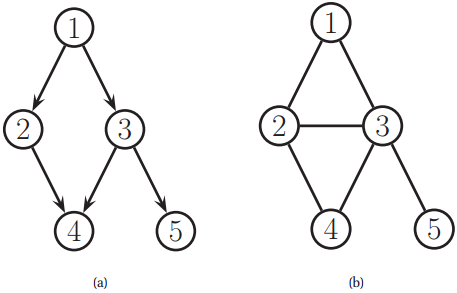
\includegraphics[scale=.50]{graphical-models.png}
\caption{(a) A simple DAG on 5 nodes, numbered in topological order. Node 1 is the root, nodes 4 and 5 are the leaves. (b) A simple undirected graph, with the following maximal cliques: {1,2,3}, {2,3,4}, {3,5}.}
\label{fig:graphical-models} 
\end{figure}


\section{Examples}


\subsection{Naive Bayes classifiers}
\begin{figure}[hbtp]
\centering
    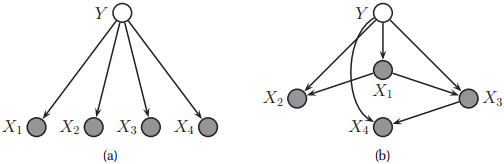
\includegraphics[scale=.60]{naive-bayes-as-DGM.png}
\caption{(a) A naive Bayes classifier represented as a DGM. We assume there are $D=4$ features, for simplicity. Shaded nodes are observed, unshaded nodes are hidden. (b) Tree-augmented naive Bayes classifier for $D=4$ features. In general, the tree topology can change depending on the value of $y$.}
\label{fig:naive-bayes-as-DGM} 
\end{figure}


\subsection{Markov and hidden Markov models}
\begin{figure}[hbtp]
\centering
    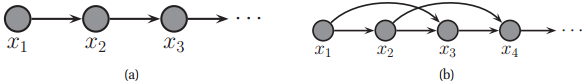
\includegraphics[scale=.50]{second-order-Markov-chain.png}
\caption{A first and second order Markov chain.}
\label{fig:second-order-Markov-chain} 
\end{figure}

\begin{figure}[hbtp]
\centering
    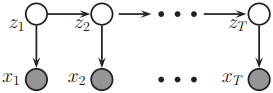
\includegraphics[scale=.60]{first-order-HMM.png}
\caption{A first-order HMM.}
\label{fig:first-order-HMM} 
\end{figure}



\section{Inference}
Suppose we have a set of correlated random variables with joint distribution $p(\vec{x}_{1:V}|\vec{\theta})$. Let us partition this vector into the \textbf{visible variables} $\vec{x}_v$, which are observed, and the \textbf{hidden variables}, $\vec{x}_h$, which are unobserved. Inference refers to computing the posterior distribution of the unknowns given the knowns:
\begin{equation}
p(\vec{x}_h|\vec{x}_v,\theta) = \frac{p(\vec{x}_h, \vec{x}_v|\vec{\theta})}{p(\vec{x}_v|\vec{\theta})}=\frac{p(\vec{x}_h, \vec{x}_v|\vec{\theta})}{\sum_{\vec{x}_h'}p(\vec{x}_h', \vec{x}_v|\vec{\theta})}
\end{equation}

Sometimes only some of the hidden variables are of interest to us. So let us partition the hidden variables into \textbf{query variables}, $\vec{x}_q$, whose value we wish to know, and the remaining \textbf{nuisance variables}, $\vec{x}_n$, which we are not interested in. We can compute what we are interested in by \textbf{marginalizing out} the nuisance variables:
\begin{equation}
p(\vec{x}_q|\vec{x}_v,\vec{\theta}) = \sum_{\vec{x}_n}p(\vec{x}_q, \vec{x}_n|\vec{x}_v, \vec{\theta})
\end{equation}


\section{Learning}
MAP estimate:
\begin{equation}
\hat{\vec{\theta}} =\arg\max_{\vec{\theta}}\sum\limits_{i=1}^N \log p(\vec{x}_{i,v}|\vec{\theta})+\log p(\vec{\theta})
\end{equation}


\subsection{Learning from complete data}
If all the variables are fully observed in each case, so there is no missing data and there are no hidden variables, we say the data is \textbf{complete}. For a DGM with complete data, the likelihood is given by
\begin{equation}\begin{split}
p(\mathcal{D}|\vec{\theta}) & = \prod_{i=1}^N p(\vec{x}_i|\vec{\theta}) \\
& = \prod_{i=1}^N\prod_{t=1}^V p(\vec{x}_{it}|\vec{x}_{i, \mathrm{pa}(t)}, \vec{\theta}_t) \\
& = \prod_{t=1}^V p(\mathcal{D}_t|\vec{\theta}_t)
\end{split}\end{equation}
where $\mathcal{D}_t$ is the data associated with node $t$ and its parents, i.e., the $t$'th family.

Now suppose that the prior factorizes as well:
\begin{equation}
p(\vec{\theta})=\prod\limits_{t=1}^V p(\vec{\theta}_t)
\end{equation}

Then clearly the posterior also factorizes:
\begin{equation}
p(\vec{\theta}|\mathcal{D}) \propto p(\mathcal{D}|\vec{\theta})p(\vec{\theta}) = \prod\limits_{t=1}^V p(\mathcal{D}_t|\vec{\theta}_t)p(\vec{\theta}_t)
\end{equation}


\subsection{Learning with missing and/or latent variables}
If we have missing data and/or hidden variables, the likelihood no longer factorizes, and indeed it is no longer convex, as we explain in detail in Section TODO. This means we will usually can only compute a locally optimal ML or MAP estimate. Bayesian inference of the parameters is even harder. We discuss suitable approximate inference techniques in later chapters.


\section{Conditional independence properties of DGMs}


\subsection{d-separation and the Bayes Ball algorithm (global Markov properties)}
\begin{enumerate}
\item P contains a chain
\begin{equation}\begin{split}
p(x,z|y) & = \frac{p(x,y,z)}{p(y)}
= \frac{p(x)p(y|x)p(z|y)}{p(y)} \\
 & = \frac{p(x,y)p(z|y)}{p(y)} = p(x|y)p(z|y)
\end{split}\end{equation}

\item P contains a fork
\begin{equation}
p(x,z|y) = \frac{p(x,y,z)}{p(y)}
= \frac{p(y)p(x|y)p(z|y)}{p(y)}
= p(x|y)p(z|y)
\end{equation}
\item P contains v-structure
\begin{equation}
p(x,z|y) = \frac{p(x,y,z)}{p(y)}
= \frac{p(x)p(z)p(y|x,z)}{p(y)}
\neq p(x|y)p(z|y)
\end{equation}
\end{enumerate}



\subsection{Other Markov properties of DGMs}


\subsection{Markov blanket and full conditionals}

\begin{equation}
mb(t) = ch(t)\cup pa(t)\cup copa(t)
\end{equation}


\subsection{Multinoulli Learning}
Multinoulli Distribution:
\begin{equation}\label{eqn:discrite}
Cat(x|\mu) = \prod_{k=1}^K\mu_k^{x_k}
\end{equation}
then from \ref{bayes_net} and \ref{eqn:discrite}:
\begin{equation}
p(x|G,\theta) = \prod_{v=1}^V\prod_{c=1}^{C_v}\prod_{k=1}^K
\theta_{vck}^{y_{vck}}
\end{equation}
Likelihood
\begin{equation}
p(D|G,\theta) = \prod_{n=1}^N p(x_n|G,\theta)
=\prod_{n=1}^N\prod_{v=1}^V\prod_{c=1}^{C_{nv}}\prod_{k=1}^K
\theta_{vck}^{y_{nvck}}
\end{equation}
where $y_{nv} = f(pa(x_{nv}))$, f(x) is a map from x to a vector, there is only one element in the vector is 1.


\section{Influence (decision) diagrams *}


\chapter{EM algorithm}
\label{chap:EM-algorithm}


\section{Jensen's inequality}

\subsection{Convex function}
\begin{definition}
A real valued function $f : X \rightarrow R$ defined on a convex set $X$ in a vector space is called \textbf{convex function} if, for any two points $\vec{x}_1$ and  $\vec{x}_2$  in $X$ and any $\lambda \in [0,1]$,
\begin{equation}
f(\lambda \vec{x}_1 + (1 - \lambda)\vec{x}_2) \leq \lambda f(\vec{x}_1) + (1 - \lambda)f(\vec{x}_2)
\end{equation}

The function $f$ is said to be \textbf{strictly convex} if
\begin{equation}
f(\lambda \vec{x}_1 + (1 - \lambda)\vec{x}_2) < \lambda f(\vec{x}_1) + (1 - \lambda)f(\vec{x}_2)
\end{equation}
\end{definition}

\begin{definition}
A function $f$ is said to be (strictly) \textbf{concave} if $-f$ is (strictly) convex.
\end{definition}

\begin{theorem}
If $f(x)$ is twice differentiable on $[a, b]$ and $f''(x) \geq 0$ on $[a, b]$ then $f(x)$ is convex on $[a, b]$.
\end{theorem}

\begin{proposition}
$\log(x)$ is strictly convex on $(0, \infty)$.
\end{proposition}


\subsection{Jensen's inequality}
\begin{theorem}
Let $f$ be a convex function defined on a convex set $X$ . If $\vec{x}_1, \vec{x}_2, \cdots , \vec{x}_n \in X$ and $\lambda_1, \lambda_2, \cdots , \lambda_n \geq 0$ with $\sum\limits_{i=1}^n \lambda_i=1$,
\begin{equation}
f\left(\sum\limits_{i=1}^n \lambda_i\vec{x}_i\right) \leq \sum\limits_{i=1}^n {\lambda_i f(\vec{x}_i)}
\end{equation}
\end{theorem}

\begin{proposition}
\begin{equation}
\log\left(\sum\limits_{i=1}^n \lambda_i\vec{x}_i\right) \geq \sum\limits_{i=1}^n {\lambda_i \log(\vec{x}_i)}
\end{equation}
\end{proposition}


\section{EM algorithm}
The EM algorithm is an efficient iterative procedure to compute the Maximum Likelihood (ML) estimate in the presence of missing or hidden data. 

Each iteration of the EM algorithm consists of two processes: The E-step, and the M-step. In the expectation, or E-step, the missing data are estimated given the observed data and current estimate of the model parameters. This is achieved using the conditional expectation, explaining the choice of terminology. In the M-step, the likelihood function is maximized under the assumption that the missing data are known. The estimate of the missing data from the E-step are used in lieu of the actual missing data.

\begin{algorithm}[htbp]
    \SetKwInOut{Input}{input}\SetKwInOut{Output}{output}
    \Input{observed data $\mathcal{X}=\{\vec{x}^{(1)},\vec{x}^{(2)},\cdots, \vec{x}^{(n)}$\},joint distribution $P(\mathcal{X},\vec{z}|\vec{\theta})$}
	\Output{model's parameters $\vec{\theta}$}

	// 1. identify hidden variables $\vec{z}$, write out the log likelihood function $\ell(\mathcal{X},\vec{z}|\vec{\theta})$ \\
	$\vec{\theta}^{(0)}$ = ... // initialize \\
	
	\While{(!convergency)} {
	    // 2. E-step: plug in $P(\mathcal{X},\vec{z}|\vec{\theta})$, derive the formula of $Q(\vec{\theta}, \vec{\theta}^{(i)})$ \\
	    $Q(\vec{\theta}, \vec{\theta}^{(i)})=\mathbb{E}_{\vec{z}|\mathcal{X},\vec{\theta}^{(i)}}\left[\log P(\mathcal{X},\vec{z}|\vec{\theta})\right]$ \\
	    // 3. M-step: find \vec{\theta} that maximizes the value of $Q(\vec{\theta}, \vec{\theta}^{(i)})$ \\
		$\vec{\theta}^{(i+1)}=\arg\max\limits_{\vec{\theta}} Q(\vec{\theta}, \vec{\theta}^{(i)})$ \\
	}
	
\caption{EM algorithm}
\end{algorithm}

\section{Derivation of the EM algorithm}
The log likelihood function is given by 
\begin{eqnarray}
\ell(\vec{\theta}) &=& \log{P(\mathcal{X}|\vec{\theta})} \text{ ,where } \log{P(\mathcal{X}|\vec{\theta})}=\sum\limits_{i=1}^{n} \log{{P(\vec{x}^{(i)}|\vec{\theta})}}\nonumber \\
                &=& \log{{\sum\limits_{\vec{z}} P(\mathcal{X},\vec{z}|\vec{\theta})}} \nonumber \\
				&=& \log{{\sum\limits_{\vec{z}} P(\mathcal{X}|\vec{z},\vec{\theta})P(\vec{z}|\vec{\theta})}} \nonumber \\
\ell(\vec{\theta})-\ell(\vec{\theta}^{(i)}) &=& \log\left[\sum\limits_{\vec{z}} P(\mathcal{X}|\vec{z},\vec{\theta})P(\vec{z}|\vec{\theta})\right] - \log{P(\mathcal{X}|\vec{\theta}^{(i)})} \nonumber \\
                &=& \log\left[\sum\limits_{\vec{z}} P(\mathcal{X}|\vec{z},\vec{\theta})P(\vec{z}|\vec{\theta})\dfrac{P(\vec{z}|\mathcal{X},\theta^{(i)})}{P(\vec{z}|\mathcal{X},\theta^{(i)})}\right] - \log{P(\mathcal{X}|\vec{\theta}^{(i)})} \nonumber \\
				&=& \log\left[\sum\limits_{\vec{z}} P(\vec{z}|\mathcal{X},\theta^{(i)})\dfrac{P(\mathcal{X}|\vec{z},\vec{\theta})P(\vec{z}|\vec{\theta})}{P(\vec{z}|\mathcal{X},\theta^{(i)})}\right] - \log{P(\mathcal{X}|\vec{\theta}^{(i)})} \nonumber \\
				&\geq& \sum\limits_{\vec{z}} P(\vec{z}|\mathcal{X},\theta^{(i)})\log\left[\dfrac{P(\mathcal{X}|\vec{z},\vec{\theta})P(\vec{z}|\vec{\theta})}{P(\vec{z}|\mathcal{X},\theta^{(i)})}\right] - \log{P(\mathcal{X}|\vec{\theta}^{(i)})} \nonumber \\
				&=& \sum\limits_{\vec{z}} P(\vec{z}|\mathcal{X},\theta^{(i)})\log\left[\dfrac{P(\mathcal{X}|\vec{z},\vec{\theta})P(\vec{z}|\vec{\theta})}{P(\vec{z}|\mathcal{X},\theta^{(i)})P(\mathcal{X}|\vec{\theta}^{(i)})}\right] \nonumber \\
				&\triangleq& B(\vec{\theta},\vec{\theta}^{(i)}) \nonumber \\
\Rightarrow \nonumber
\end{eqnarray}

\begin{eqnarray}
\vec{\theta}^{(i+1)} &=& \arg\max\limits_{\vec{\theta}}{\left[ \ell(\vec{\theta}^{(i)})+B(\vec{\theta},\vec{\theta}^{(i)})\right]} \nonumber \\
                &=& \arg\max\limits_{\vec{\theta}}{\left\{ \ell(\vec{\theta}^{(i)})+\sum\limits_{\vec{z}} P(\vec{z}|\mathcal{X},\theta^{(i)})\log\left[\dfrac{P(\mathcal{X}|\vec{z},\vec{\theta})P(\vec{z}|\vec{\theta})}{P(\vec{z}|\mathcal{X},\theta^{(i)})P(\mathcal{X}|\vec{\theta}^{(i)})}\right]\right\}} \nonumber \\
				&& \text{Now drop terms which are constant w.r.t. } \vec{\theta} \nonumber \\
				&=& \arg\max\limits_{\vec{\theta}}{\left\{\sum\limits_{\vec{z}} P(\vec{z}|\mathcal{X},\theta^{(i)})\log\left[P(\mathcal{X}|\vec{z},\vec{\theta})P(\vec{z}|\vec{\theta})\right]\right\}} \nonumber \\
				&=& \arg\max\limits_{\vec{\theta}}{\left\{\sum\limits_{\vec{z}} P(\vec{z}|\mathcal{X},\theta^{(i)})\log\left[P(\mathcal{X},\vec{z}|\vec{\theta})\right]\right\}} \nonumber \\
				&=& \arg\max\limits_{\vec{\theta}}{\left\{\mathbb{E}_{\vec{z}|\mathcal{X},\theta^{(i)}}\log\left[P(\mathcal{X},\vec{z}|\vec{\theta})\right]\right\}} \\
				&\triangleq& \arg\max\limits_{\vec{\theta}}{Q(\vec{\theta}, \vec{\theta}^{(i)})}
\end{eqnarray}

\begin{figure}[hbtp]
\centering
    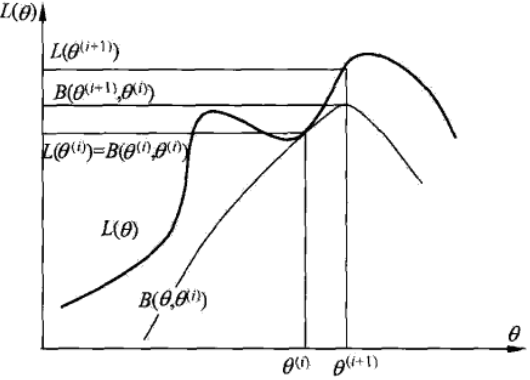
\includegraphics[scale=.50]{EM-algorithm.png}
\caption{Graphical interpretation of a single iteration of the EM algorithm: The function $B(\vec{\theta},\vec{\theta}^{(i)})$ is bounded above by the log likelihood function $\ell(\vec{\theta})$. The functions are equal at $\vec{\theta} = \vec{\theta}^{(i)}$. The EM algorithm chooses $\vec{\theta}^{(i)}$ as the value of $\vec{\theta}$ for which $B(\vec{\theta},\vec{\theta}^{(i)})$ is a maximum. Since $\ell(\vec{\theta}) \geq B(\vec{\theta},\vec{\theta}^{(i)})$ increasing $B(\vec{\theta},\vec{\theta}^{(i)})$ ensures that the value of the log likelihood function $\ell(\vec{\theta})$ is increased at each step.}
\label{fig:EM-algorithm} 
\end{figure}


\section{Examples}

\subsection{Gaussian mixture model}
\begin{definition}
In Gaussian mixture model(GMM) model, each base distribution in the mixture is a multivariate Gaussian with mean $\mu_k$ and covariance matrix $\sigma_k$. Thus the model has the form
\begin{equation}
P(x_i|\vec{\theta})=\sum\limits_{k=1}^K{\pi_k\phi(x_i|\mu_k,\sigma_k)}
\end{equation}
\end{definition}

Figure ~\ref{fig:GMM} shows a mixture of 3 Gaussians in 2D. Each mixture component is represented by a different set of eliptical contours. Given a sufficiently large number of mixture components, a GMM can be used to approximate any density defined on $\mathbb{R}^D$.

\begin{figure}[hbtp]
\centering
    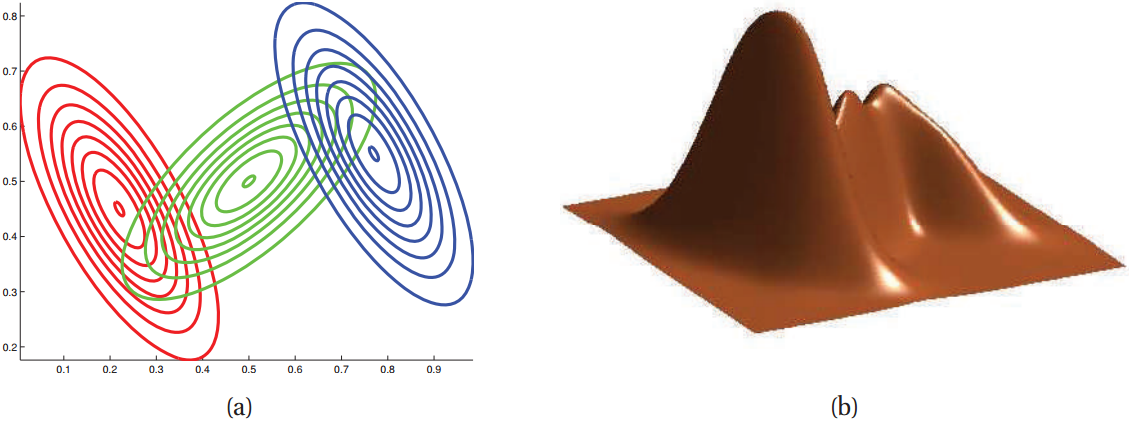
\includegraphics[scale=.50]{GMM.png}
\caption{A mixture of 3 Gaussians in 2d. (a) We show the contours of constant probability for eachcomponent in the mixture. (b) A surface plot of the overall density.}
\label{fig:GMM} 
\end{figure}


\subsubsection{Identify hidden variable, write out the log likelihood function}
Denote the hidden variable as $\gamma_{jk}$, which's meanining is:
\begin{equation}\nonumber
\gamma_{jk}=\begin{cases}
1, & \text{the j-th sample comes from the k-th model}\\
0, & \text{otherwise} \\
\end{cases}
\end{equation}

Given observed sample $x_j$ and hidden variable $\gamma_{jk}$, the complete sample is $(x_j,\gamma_{j1},\gamma_{j1},\cdots,\gamma_{jk})$.

Then the log likelihood function can be written as follows:
\begin{eqnarray}
P(\mathcal{X},\gamma|\vec{\theta}) &=& \prod\limits_{j=1}^N P(x_j,\gamma_{j1},\gamma_{j1},\cdots,\gamma_{jk}|\vec{\theta})\nonumber \\
       &=& \prod\limits_{j=1}^N\left\{\prod\limits_{k=1}^K\left[\pi_k\phi(x_i|\mu_k,\sigma_k)\right]^{\gamma_{jk}}\right\} \nonumber \\
	   &=& \prod\limits_{k=1}^K\left\{\prod\limits_{j=1}^N\left[\pi_k\phi(x_i|\mu_k,\sigma_k)\right]^{\gamma_{jk}}\right\} \nonumber \\
	   &=& \prod\limits_{k=1}^K\left\{\pi_k^{n_k}\prod\limits_{j=1}^N\left[\phi(x_i|\mu_k,\sigma_k)\right]^{\gamma_{jk}}\right\} \nonumber \\
	   &=& \prod\limits_{k=1}^K\left\{\pi_k^{n_k}\prod\limits_{j=1}^N\left[\dfrac{1}{\sqrt{2\pi}\Sigma_k}\exp{\left(-\dfrac{\left(x_j-\mu_k\right)^2}{2\sigma_k^2}\right)}\right]^{\gamma_{jk}}\right\} \nonumber \\
	   && \text{where } n_k=\sum\limits_{j=1}^N{\gamma_{jk}}, \sum\limits_{k=1}^K{n_k}=N. \nonumber \\
\Rightarrow \nonumber \\
\log{P(\mathcal{X},\gamma|\vec{\theta})} &=& \sum\limits_{k=1}^K\left\{n_k\log\pi_k+\sum\limits_{j=1}^N{\gamma_{jk}\left[\log(\dfrac{1}{\sqrt{2\pi}}-\log\sigma_k-\dfrac{\left(x_j-\mu_k\right)^2}{2\sigma_k^2})\right]}\right\}
\end{eqnarray}


\subsubsection{E-step: derive the formula of $Q(\vec{\theta}, \vec{\theta}^{(i)})$}
\begin{eqnarray}
Q(\vec{\theta}, \vec{\theta}^{(i)}) &=& \mathbb{E}_{\vec{z}|\mathcal{X},\theta^{(i)}}\log\left[P(\mathcal{X},\vec{z}|\vec{\theta})\right] \nonumber \\
    &=& \mathbb{E}_{\vec{\gamma}|\mathcal{X},\theta^{(i)}}\left\{\sum\limits_{k=1}^K\left\{n_k\log\pi_k+\sum\limits_{j=1}^N{\gamma_{jk}\left[\log(\dfrac{1}{\sqrt{2\pi}}-\log\sigma_k-\dfrac{\left(x_j-\mu_k\right)^2}{2\sigma_k^2})\right]}\right\}\right\} \nonumber \\
	&=& \sum\limits_{k=1}^K\left\{\left(\sum\limits_{j=1}^N{E\gamma_{jk}}\right)\log\pi_k+\sum\limits_{j=1}^N{E\gamma_{jk}\left[\log(\dfrac{1}{\sqrt{2\pi}}-\log\sigma_k-\dfrac{\left(x_j-\mu_k\right)^2}{2\sigma_k^2})\right]}\right\} \nonumber \\
	&& \text{denote } E\gamma_{jk} \text{ as } \hat{\gamma}_{jk} \nonumber \\
	&=& \sum\limits_{k=1}^K\left\{\left(\sum\limits_{j=1}^N{\hat{\gamma}_{jk}}\right)\log\pi_k+\sum\limits_{j=1}^N{\hat{\gamma}_{jk}\left[\log(\dfrac{1}{\sqrt{2\pi}}-\log\sigma_k-\dfrac{\left(x_j-\mu_k\right)^2}{2\sigma_k^2})\right]}\right\} \label{eqn:Q-function} \label{eqn:Q-function}
\end{eqnarray}

\begin{eqnarray}
\hat{\gamma}_{jk} &=& E\gamma_{jk} = E(\gamma_{jk}|x_j,\vec{\theta})=E(\gamma_{jk}=1|x_j,\vec{\theta}) \nonumber \\
	&=& \dfrac{P(\gamma_{jk}=1, x_j|\vec{\theta})}{\sum\limits_{k=1}^K{P(\gamma_{jk}=1, x_j|\vec{\theta})}} \nonumber \\
	&=& \dfrac{P(x_j|\gamma_{jk}=1, \vec{\theta})P(\gamma_{jk}=1, \vec{\theta})}{\sum\limits_{k=1}^K{P(x_j|\gamma_{jk}=1, \vec{\theta})P(\gamma_{jk}=1, \vec{\theta})}} \nonumber \\
	&=& \dfrac{\phi(x_i|\mu_k,\sigma_k)\pi_k}{\sum\limits_{k=1}^K{\phi(x_i|\mu_k,\sigma_k)\pi_k}} \nonumber \\
	&=& \dfrac{\pi_k\phi(x_i|\mu_k,\sigma_k)}{\sum\limits_{k=1}^K{\pi_k\phi(x_i|\mu_k,\sigma_k)}} \nonumber
\end{eqnarray}
Use this formula to update $\hat{\gamma}_{jk}$.

\subsubsection{M-step: find \vec{\theta} that maximizes the value of $Q(\vec{\theta}, \vec{\theta}^{(i)})$}
Take partial derivatives of Eqn.\eqref{eqn:Q-function} with respect to $\mu_k$, $\sigma_k^2$ and let them equal to 0, we can get $\mu_k$, $\sigma_k^2$.
\begin{eqnarray}
\dfrac{\partial}{\partial \mu_k}Q(\vec{\theta}, \vec{\theta}^{(i)}) &=& \sum\limits_{j=1}^N{\hat{\gamma}_{jk}\left[-\dfrac{1}{2\sigma_k^2} \cdot 2\left(x_j-\mu_k\right) \cdot (-1)\right]} = 0 \nonumber \\
\sum\limits_{j=1}^N{\hat{\gamma}_{jk}\left[\left(x_j-\mu_k\right)\right]} &=& 0 \nonumber \\
\hat{\mu}_k &=& \dfrac{\sum\limits_{j=1}^N{\hat{\gamma}_{jk}x_j}}{\hat{\gamma}_{jk}}
\end{eqnarray}

\begin{eqnarray}
\dfrac{\partial}{\partial \sigma_k^2}Q(\vec{\theta}, \vec{\theta}^{(i)}) &=& \sum\limits_{j=1}^N{\hat{\gamma}_{jk}\left[-\dfrac{1}{2\sigma_k^2}+\dfrac{1}{2\sigma_k^4}\left(x_j-\mu_k\right)^2\right]} = 0 \nonumber \\
\sum\limits_{j=1}^N{\hat{\gamma}_{jk}\left[-\sigma_k^2+\left(x_j-\mu_k\right)^2\right]} &=& 0 \nonumber \\
\hat{\sigma}_k^2 &=& \dfrac{\sum\limits_{j=1}^N{\hat{\gamma}_{jk}\left(x_j-\mu_k\right)^2}}{\hat{\gamma}_{jk}}
\end{eqnarray}

Grouping together only the terms that depend on $\pi_k$, we find that we need to maximize $\sum\limits_{k=1}^K{\left(\sum\limits_{j=1}^N{\hat{\gamma}_{jk}}\right)\log\pi_k}$. However, there is an additional constraint $\sum\limits_{k=1}^K{\pi_k}=1$, since they represent the probabilities $\vec{\pi}_k=P(x^{(i)}=k|\vec{\pi})$. To deal with the constraint we construct the Lagrangian
\begin{equation}
\mathcal{L}(\vec{\pi})=\sum\limits_{k=1}^K{\left(\sum\limits_{j=1}^N{\hat{\gamma}_{jk}}\right)\log\pi_k}+\beta\left(\sum\limits_{k=1}^K{\pi_k}-1\right) \nonumber
\end{equation}

where $\beta$ is the Lagrange multiplier. Taking derivatives, we find
\begin{equation}
\hat{\vec{\pi}}_k=\dfrac{\sum\limits_{k=1}^K{\hat{\gamma}_{jk}}}{N}
\end{equation}


\subsubsection{EM algorithm for GMM}

\begin{algorithm}[htbp]
    \SetAlgoNoLine
    \SetKwInOut{Input}{input}\SetKwInOut{Output}{output}
    \Input{observed data $\mathcal{X}=\{\vec{x}^{(1)},\vec{x}^{(2)},\cdots, \vec{x}^{(n)}$\},GMM}
	\Output{GMM's parameters $\vec{\pi},\vec{\mu},\vec{\sigma}$}

	// 1. initialize \\
	$\vec{\pi}^{(0)}$ = ... \\
	$\vec{\mu}^{(0)}$ = ...  \\
	$\vec{\sigma}^{(0)}$ = ...  \\
	
	\While{(!convergency)} {
	    // 2. E-step \\
	    $\hat{\gamma}_{jk}=\dfrac{\pi_k\phi(x_i|\mu_k,\sigma_k)}{\sum\limits_{k=1}^K{\pi_k\phi(x_i|\mu_k,\sigma_k)}}$ \\
	    // 3. M-step \\
		$\hat{\mu}_k = \dfrac{\sum\limits_{j=1}^N{\hat{\gamma}_{jk}x_j}}{\hat{\gamma}_{jk}}$ \\
		$\hat{\sigma}_k^2 = \dfrac{\sum\limits_{j=1}^N{\hat{\gamma}_{jk}\left(x_j-\mu_k\right)^2}}{\hat{\gamma}_{jk}}$ \\
		$\hat{\vec{\pi}}_k=\dfrac{\sum\limits_{k=1}^K{\hat{\gamma}_{jk}}}{N}$ \\
	}
	
\caption{EM algorithm for GMM}
\end{algorithm}


\section{Generalization of EM Algorithm}
EM algorithm can be interpreted as F function's maximization-maximization algorithm, based on this interpretation there are many variations and generalization, e.g., generalized EM Algorithm(GEM).


\subsection{F function's maximization-maximization algorithm}
\begin{definition}
Given the probability distribution of the hidden variable $Z$ is $\tilde{P}(Z)$, define \textbf{F function} as the following:
\begin{equation}
F(\tilde{P},\vec{\theta})=\mathbb{E}_{\tilde{P}}\left[\log{P(X,Z|\theta)}\right]+H(\tilde{P})
\end{equation}
Where $H(\tilde{P})=-\mathbb{E}_{\tilde{P}}\log\tilde{P}(Z)$, which is $\tilde{P}(Z)$'s entropy. Usually we assume that $P(X,Z|\theta)$ is continuous w.r.t. $\vec{\theta}$, therefore $F(\tilde{P},\vec{\theta})$ is continuous w.r.t. $\tilde{P}$ and $\vec{\theta}$.
\end{definition}

\begin{lemma}
\label{lemma:F-function}
For a fixed $\vec{\theta}$, there is only one distribution $\tilde{P}_{\theta}$ which maximizes $F(\tilde{P},\vec{\theta})$
\begin{equation}
\tilde{P}_{\theta}(Z)=P(Z|X, \vec{\theta})
\end{equation}
and $\tilde{P}_{\theta}$ is continuous w.r.t. $\vec{\theta}$.
\end{lemma}

\begin{proof}
Given a fixed $\vec{\theta}$, we can get $\tilde{P}_{\theta}$ which maximizes $F(\tilde{P},\vec{\theta})$. we construct the Lagrangian
\begin{equation}
\mathcal{L}(\tilde{P}, \vec{\theta})=\mathbb{E}_{\tilde{P}}\left[\log{P(X,Z|\theta)}\right]-\mathbb{E}_{\tilde{P}}\log\tilde{P}_{\theta}(Z)+\lambda\left[1-\sum\limits_Z{\tilde{P}(Z)}\right]
\end{equation}

Take partial derivative with respect to $\tilde{P}_{\theta}(Z)$ then we get
\begin{equation}
\dfrac{\partial \mathcal{L}}{\partial{\tilde{P}_{\theta}(Z)}}=\log{P(X,Z|\theta)}-\log\tilde{P}_{\theta}(Z)-1-\lambda  \nonumber
\end{equation}

Let it equal to 0, we can get
\begin{equation}
\lambda=\log{P(X,Z|\theta)}-\log\tilde{P}_{\theta}(Z)-1 \nonumber
\end{equation}

Then we can derive that $\tilde{P}_{\theta}(Z)$ is proportional to $P(X,Z|\theta)$
\begin{eqnarray}
\dfrac{P(X,Z|\theta)}{\tilde{P}_{\theta}(Z)} &=& e^{1+\lambda} \nonumber \\
\Rightarrow \tilde{P}_{\theta}(Z) &=& \dfrac{P(X,Z|\vec{\theta})}{e^{1+\lambda}} \nonumber \\
\sum\limits_Z{\tilde{P}_{\theta}(Z)}=1 & \Rightarrow & \sum\limits_Z{\dfrac{P(X,Z|\vec{\theta})}{e^{1+\lambda}}}=1 \Rightarrow P(X|\vec{\theta})=e^{1+\lambda} \nonumber \\
\tilde{P}_{\theta}(Z) &=& \dfrac{P(X,Z|\vec{\theta})}{e^{1+\lambda}} = \dfrac{P(X,Z|\vec{\theta})}{P(X|\vec{\theta})}=P(Z|X, \vec{\theta}) \nonumber
\end{eqnarray}
\end{proof}

\begin{lemma}
If $\tilde{P}_{\theta}(Z)=P(Z|X, \vec{\theta})$, then
\begin{equation}
F(\tilde{P},\vec{\theta})=\log P(X|\vec{\theta})
\end{equation}
\end{lemma}

\begin{theorem}
One iteration of EM algorithm can be implemented as F function's maximization-maximization.

Assume $\vec{\theta}^{(i)}$ is the estimation of $\vec{\theta}$ in the i-th iteration, $\tilde{P}^{(i)}$ is the estimation of $\tilde{P}$ in the i-th iteration. Then in the (i+1)-th iteration two steps are:
\begin{enumerate}
\item for fixed $\vec{\theta}^{(i)}$, find $\tilde{P}^{(i+1)}$ that maximizes $F(\tilde{P},\vec{\theta}^{(i)})$;
\item for fixed $\tilde{P}^{(i+1)}$, find $\vec{\theta}^{(i+1)}$ that maximizes $F(\tilde{P}^{(i+1)},\vec{\theta})$.
\end{enumerate}
\end{theorem}

\begin{proof}
(1) According to Lemma \ref{lemma:F-function}, we can get
\begin{equation}
\tilde{P}^{(i+1)}(Z)=P(Z|X, \vec{\theta}^{(i)}) \nonumber
\end{equation}

(2) According above, we can get
\begin{eqnarray}
F(\tilde{P}^{(i+1)},\vec{\theta}) &=& \mathbb{E}_{\tilde{P}^{(i+1)}}\left[\log{P(X,Z|\theta)}\right]+H(\tilde{P}^{(i+1)}) \nonumber \\
    &=& \sum\limits_Z{P(Z|X,\vec{\theta}^{(i)})\log{P(X,Z|\theta)}}+H(\tilde{P}^{(i+1)}) \nonumber \\
	&=& Q(\vec{\theta}, \vec{\theta}^{(i)})+H(\tilde{P}^{(i+1)})\nonumber
\end{eqnarray}

Then
\begin{equation}
\vec{\theta}^{(i+1)}=\arg\max\limits_{\theta}F(\tilde{P}^{(i+1)},\vec{\theta})=\arg\max\limits_{\theta}Q(\vec{\theta}, \vec{\theta}^{(i)}) \nonumber
\end{equation}
\end{proof}


\subsection{The Generalized EM Algorithm(GEM)}
In the formulation of the EM algorithm described above, $\vec{\theta}^{(i+1)}$ was chosen as the value of $\vec{\theta}$ for which $Q(\vec{\theta}, \vec{\theta}^{(i)})$ was maximized. While this ensures the greatest increase in $\ell(\vec{\theta})$, it is however possible to relax the requirement of maximization to one of simply increasing $Q(\vec{\theta}, \vec{\theta}^{(i)})$ so that $Q(\vec{\theta}^{(i+1)}, \vec{\theta}^{(i)}) \geq Q(\vec{\theta}^{(i)}, \vec{\theta}^{(i)})$. This approach, to simply increase and not necessarily maximize $Q(\vec{\theta}^{(i+1)}, \vec{\theta}^{(i)})$ is known as the Generalized Expectation Maximization (GEM) algorithm and is often useful in cases where the maximization is difficult. The convergence of the GEM algorithm is similar to the EM algorithm.


\section{Reference}
[1] Dempster AP, Laird NM, Rubin DB. Maximum-likelihood from incomplete data via the EM algorithm. J.Royal Statist. Soc. Ser.B., 1977, 39

[2] Sean Borman. The Expectation Maximization Algorithm A short tutorial. 2009. \url{http://www.seanborman.com/publications/EM_algorithm.pdf}
\chapter{Latent linear models}


\section{Factor analysis}
One problem with mixture models is that they only use a single latent variable to generate the observations. In particular, each observation can only come from one of $K$ prototypes. One can think of a mixture model as using $K$ hidden binary variables, representing a one-hot encoding of the cluster identity. But because these variables are mutually exclusive, the model is still limited in its representational power.

An alternative is to use a vector of real-valued latent variables,$\vec{z}_i \in \mathbb{R}^L$. The simplest prior to use is a Gaussian (we will consider other choices later):
\begin{equation}\label{eqn:FA-prior}
p(\vec{z}_i)=\mathcal{N}(\vec{z}_i|\vec{\mu}_0,\vec{\Sigma}_0)
\end{equation}
If the observations are also continuous, so $\vec{x}_i \in \mathbb{R}^D$, we may use a Gaussian for the likelihood. Just as in linear regression, we will assume the mean is a linear function of the (hidden) inputs, thus yielding
\begin{equation}\label{eqn:FA-class-conditional-density}
p(\vec{x}_i|\vec{z}_i,\vec{\theta})=\mathcal{N}(\vec{x}_i|\vec{W}\vec{z}_i+\vec{\mu},\vec{\Psi})
\end{equation}
where \vec{W} is a $D \times L$ matrix, known as the \textbf{factor loading matrix}, and $\vec{\Psi}$ is a $D \times D$ covariance matrix. We take $\vec{\Psi}$ to be diagonal, since the whole point of the model is to “force” $\vec{z}_i$ to explain the correlation, rather than “baking it in” to the observation’s covariance. This overall model is called \textbf{factor analysis} or \textbf{FA}. The special case in which $\vec{\Psi}=\sigma^2\vec{I}$ is called \textbf{probabilistic principal components analysis} or \textbf{PPCA}. The reason for this name will become apparent later.


\subsection{FA is a low rank parameterization of an MVN}
FA can be thought of as a way of specifying a joint density model on $\vec{x}$ using a small number of parameters. To see this, note that from Equation \eqref{eqn:Linear-Gaussian-system-normalizer}, the induced marginal distribution $p(\vec{x}_i|\vec{\theta})$ is a Gaussian:
\begin{align}
p(\vec{x}_i|\vec{\theta}) & = \int \mathcal{N}(\vec{x}_i|\vec{W}\vec{z}_i+\vec{\mu},\vec{\Psi})\mathcal{N}(\vec{z}_i|\vec{\mu}_0,\vec{\Sigma}_0)\mathrm{d}\vec{z}_i \nonumber \\
 & = \mathcal{N}(\vec{x}_i|\vec{W}\vec{\mu}_0+\vec{\mu},\vec{\Psi}+\vec{W}\vec{\Sigma}_0\vec{W})
\end{align}
From this, we see that we can set $\vec{\mu}_0=0$ without loss of generality, since we can always absorb $\vec{W}\vec{\mu}_0$ into $\vec{\mu}$. Similarly, we can set $\vec{\Sigma}_0=\vec{I}$ without loss of generality, because we can always “emulate” a correlated prior by using defining a new weight matrix, $\tilde{\vec{W}}=\vec{W}\vec{\Sigma}_0^{-\frac{1}{2}}$. So we can rewrite Equation \eqref{eqn:FA-prior} and \eqref{eqn:FA-class-conditional-density} as:
\begin{align}
p(\vec{z}_i)&=\mathcal{N}(\vec{z}_i|\vec{0},\vec{I}) \\
p(\vec{x}_i|\vec{z}_i,\vec{\theta})&=\mathcal{N}(\vec{x}_i|\vec{W}\vec{z}_i+\vec{\mu},\vec{\Psi})
\end{align}

We thus see that FA approximates the covariance matrix of the visible vector using a low-rank decomposition:
\begin{equation}\label{eqn:FA-prior}
\vec{C} \triangleq \mathrm{cov}[\vec{x}]=\vec{W}\vec{W}^T+\vec{\Psi}
\end{equation}
This only uses $O(LD)$ parameters, which allows a flexible compromise between a full covariance Gaussian, with $O(D^2)$ parameters, and a diagonal covariance, with $O(D)$ parameters. Note that if we did not restrict $\vec{\Psi}$ to be diagonal, we could trivially set $\vec{\Psi}$ to a full covariance matrix; then we could set $\vec{W}=0$, in which case the latent factors would not be required.


\subsection{Inference of the latent factors}
\begin{align}
p(\vec{z}_i|\vec{x}_i,\vec{\theta}) & = \mathcal{N}(\vec{z}_i|\vec{\mu}_i,\vec{\Sigma}_i) \\
\vec{\Sigma}_i & \triangleq (\vec{\Sigma}_0^{-1}+\vec{W}^T\vec{\Psi}^{-1}\vec{W})^{-1} \\
               & =(\vec{I}+\vec{W}^T\vec{\Psi}^{-1}\vec{W})^{-1} \\
\vec{\mu}_i & \triangleq \vec{\Sigma}_i[\vec{W}^T\vec{\Psi}^{-1}(\vec{x}_i-\vec{\mu})+\vec{\Sigma}_0^{-1}\vec{\mu}_0] \\
            & =\vec{\Sigma}_i\vec{W}^T\vec{\Psi}^{-1}(\vec{x}_i-\vec{\mu})
\end{align}
Note that in the FA model, $\vec{\Sigma}_i$ is actually independent of $i$, so we can denote it by $\vec{\Sigma}$. Computing this matrix takes $O(L^3+L^2D)$ time, and computing each $\vec{\mu}_i=\mathbb{E}[\vec{z}_i|\vec{x}_i,\vec{\theta}]$ takes $O(L^2+LD)$ time. The $\vec{\mu}_i$ are sometimes called the \textbf{latent scores}, or \textbf{latent factors}.


\subsection{Unidentifiability}
Just like with mixture models, FA is also unidentifiable. To see this, suppose $\vec{R}$ is an arbitrary orthogonal rotation matrix, satisfying $\vec{R}\vec{R}^T=\vec{I}$. Let us define $\tilde{\vec{W}}=\vec{W}\vec{R}$, then the likelihood function of this modified matrix is the same as for the unmodified matrix, since $\vec{W}\vec{R}\vec{R}^T\vec{W}^T+\vec{\Psi}=\vec{W}\vec{W}^T+\vec{\Psi}$. Geometrically, multiplying $\vec{W}$ by an orthogonal matrix is like rotating $\vec{z}$ before generating $\vec{x}$.

To ensure a unique solution, we need to remove $L(L-1)/2$ degrees of freedom, since that is the number of orthonormal matrices of size $L \times L$.\footnote{To see this, note that there are $L-1$ free parameters in $\vec{R}$ in the first column (since the column vector must be normalized to unit length), there are $L-2$ free parameters in the second column (which must be orthogonal to the first), and so on.} In total, the FA model has $D+LD-L(L-1)/2$ free parameters (excluding the mean), where the first term arises from $\vec{\Psi}$. Obviously we require this to be less than or equal to $D(D+1)/2$, which is the number of parameters in an unconstrained (but symmetric) covariance matrix. This gives us an upper bound on $L$, as follows:
\begin{equation}
L_{\mathrm{max}}=\lfloor D+0.5(1-\sqrt{1+8D}) \rfloor
\end{equation}

For example, $D=6$ implies $L \leq 3$. But we usually never choose this upper bound, since it would result in overfitting (see discussion in Section \ref{sec:FA-Choosing-L} on how to choose $L$).


Unfortunately, even if we set $L < L_{\mathrm{max}}$, we still cannot uniquely identify the parameters, since the rotational ambiguity still exists. Non-identifiability does not affect the predictive performance of the model. However, it does affect the loading matrix, and hence the interpretation of the latent factors. Since factor analysis is often used to uncover structure in the data, this problem needs to be addressed. Here are some commonly used solutions:
\begin{itemize}
\item{\textbf{Forcing $\vec{W}$ to be orthonormal} Perhaps the cleanest solution to the identifiability problem is to force $\vec{W}$ to be orthonormal, and to order the columns by decreasing variance of the corresponding latent factors. This is the approach adopted by PCA, which we will discuss in Section \ref{sec:PCA}. The result is not necessarily more interpretable, but at least it is unique.}
\item{\textbf{Forcing $\vec{W}$ to be lower triangular} One way to achieve identifiability, which is popular in the Bayesian community (e.g., (Lopes and West 2004)), is to ensure that the first visible feature is only generated by the first latent factor, the second visible feature is only generated by the first two latent factors, and so on. For example, if $L=3$ and $D=4$, the correspond factor loading matrix is given by
\begin{equation*}
\vec{W}=\left(\begin{array}{ccc}
w_{11} & 0 & 0 \\
w_{21} & w_{22} & 0 \\
w_{31} & w_{32} & w_{33} \\
w_{41} & w_{32} & w_{43}
\end{array}\right)
\end{equation*}
We also require that $w_{jj} >0$ for $j =1:L$. The total number of parameters in this constrained matrix is $D+DL-L(L-1)/2$, which is equal to the number of uniquely identifiable parameters. The disadvantage of this method is that the first $L$ visible variables, known as the \textbf{founder variables}, affect the interpretation of the latent factors, and so must be chosen carefully.}
\item{\textbf{Sparsity promoting priors on the weights} Instead of pre-specifying which entries in $\vec{W}$ are zero, we can encourage the entries to be zero, using $\ell_1$ regularization (Zou et al. 2006), ARD (Bishop 1999; Archambeau and Bach 2008), or spike-and-slab priors (Rattray et al. 2009). This is called sparse factor analysis. This does not necessarily ensure a unique MAP estimate, but it does encourage interpretable solutions. See Section 13.8 TODO.}
\item{\textbf{Choosing an informative rotation matrix} There are a variety of heuristic methods that try to find rotation matrices $\vec{R}$ which can be used to modify $\vec{W}$(and hence the latent factors) so as to try to increase the interpretability, typically by encouraging them to be (approximately) sparse. One popular method is known as \textbf{varimax}(Kaiser 1958).}
\item{\textbf{Use of non-Gaussian priors for the latent factors} In Section \ref{sec:ICA}, we will dicuss how replacing $p(\vec{z}_i)$ with a non-Gaussian distribution can enable us to sometimes uniquely identify $\vec{W}$ as well as the latent factors. This technique is known as ICA.}
\end{itemize}


\subsection{Mixtures of factor analysers}
The FA model assumes that the data lives on a low dimensional linear manifold. In reality, most
data is better modeled by some form of low dimensional \emph{curved} manifold. We can approximate a curved manifold by a piecewise linear manifold. This suggests the following model: let the $k$'th linear subspace of dimensionality $L_k$ be represented by $\vec{W}_k$, for $k=1:K$. Suppose we have a latent indicator $qi \in \{1,\cdots,K\}$ specifying which subspace we should use to generate the data. We then sample $\vec{z}_i$ from a Gaussian prior and pass it through the $\vec{W}_k$ matrix (where $k=q_i$), and add noise. More precisely, the model is as follows:
\begin{align}
p(q_i|\vec{\theta}) & =\mathrm{Cat}(q_i\vec{\pi}) \\
p(\vec{z}_i|\vec{\theta}) & =\mathcal{N}(\vec{z}_i|\vec{0},\vec{I}) \\
p(\vec{x}_i|q_i=k,\vec{z}_i,\vec{\theta}) & =\mathcal{N}(\vec{x}_i|\vec{W}\vec{z}_i+\vec{\mu}_k,\vec{\Psi})
\end{align}
This is called a \textbf{mixture of factor analysers}(MFA) (Hinton et al. 1997).

Another way to think about this model is as a low-rank version of a mixture of Gaussians. In particular, this model needs $O(KLD)$ parameters instead of the $O(KD^2)$ parameters needed for a mixture of full covariance Gaussians. This can reduce overfitting. In fact, MFA is a good generic density model for high-dimensional real-valued data.


\subsection{EM for factor analysis models}
Below we state the results without proof. The derivation can be found in (Ghahramani and Hinton 1996a). To obtain the results for a single factor analyser, just set $r_{ic} =1$ and $c=1$ in the equations below. In Section \ref{sec:EM-for-PCA} we will see a further simplification of these equations that arises when fitting a PPCA model, where the results will turn out to have a particularly simple and elegant interpretation.

In the E-step, we compute the posterior responsibility of cluster $k$ for data point $i$ using
\begin{equation}
r_{ik} \triangleq p(q_i=k|\vec{x}_i,\vec{\theta}) \propto \pi_k\mathcal{N}(\vec{x}_i|\vec{\mu}_k,\vec{W}_k\vec{W}_k^T\vec{\Psi}_k)
\end{equation}

The conditional posterior for $\vec{z}_i$ is given by
\begin{align}
p(\vec{z}_i|\vec{x}_i,q_i=k,\vec{\theta}) & = \mathcal{N}(\vec{z}_i|\vec{\mu}_{ik},\vec{\Sigma}_{ik}) \\
\vec{\Sigma}_{ik} & \triangleq (\vec{I}+\vec{W}_k^T\vec{\Psi}_k^{-1}\vec{W})_k^{-1} \\
\vec{\mu}_{ik} & \triangleq \vec{\Sigma}_{ik}\vec{W}_k^T\vec{\Psi}_k^{-1}(\vec{x}_i-\vec{\mu}_k)
\end{align}

In the M step, it is easiest to estimate $\vec{\mu}_k$ and $\vec{W}_k$ at the same time, by defining $\tilde{\vec{W}}_k=(\vec{W}_k,\vec{\mu}_k)$, $\tilde{\vec{z}}=(\vec{z},1)$, also, define
\begin{align}
\tilde{\vec{W}}_k & =(\vec{W}_k,\vec{\mu}_k) \\
\tilde{\vec{z}} & =(\vec{z},1) \\
\vec{b}_{ik} & \triangleq \mathbb{E}[\tilde{\vec{z}}|\vec{x}_i,q_i=k]=\mathbb{E}[(\vec{\mu}_{ik};1)] \\
\vec{C}_{ik} & \triangleq \mathbb{E}[\tilde{\vec{z}}\tilde{\vec{z}}^T|\vec{x}_i,q_i=k] \\
    & =\left(\begin{array}{cc}
\mathbb{E}[\vec{z}\vec{z}^T|\vec{x}_i,q_i=k] & \mathbb{E}[\vec{z}|\vec{x}_i,q_i=k] \\
\mathbb{E}[\vec{z}|\vec{x}_i,q_i=k]^T & 1
\end{array}\right)
\end{align}
Then the M step is as follows:
\begin{align}
\hat{\pi}_k & = \frac{1}{N}\sum\limits_{i=1}^N r_{ik} \\
\hat{\tilde{\vec{W}}}_k & = \left(\sum\limits_{i=1}^N r_{ik}\vec{x}_i\vec{b}_{ik}^T\right)\left(\sum\limits_{i=1}^N r_{ik}\vec{x}_i\vec{C}_{ik}^T\right)^{-1} \label{eqn:FA-EM-W} \\
\hat{\vec{\Psi}} & = \frac{1}{N}\mathrm{diag}\left[\sum\limits_{i=1}^N r_{ik}(\vec{x}_i-\hat{\tilde{\vec{W}}}_{ik}\vec{b}_{ik})\vec{x}_i^T\right]
\end{align}

Note that these updates are for “vanilla” EM. A much faster version of this algorithm, based on ECM, is described in (Zhao and Yu 2008).


\subsection{Fitting FA models with missing data}
\label{sec:Fitting-FA-models-with-missing-data}
In many applications, such as collaborative filtering, we have missing data. One virtue of the EM approach to fitting an FA/PPCA model is that it is easy to extend to this case. However, overfitting can be a problem if there is a lot of missing data. Consequently it is important to perform MAP estimation or to use Bayesian inference. See e.g., (Ilin and Raiko 2010) for details.


\section{Principal components analysis (PCA)}
\label{sec:PCA}
Consider the FA model where we constrain $\vec{\Psi}=\sigma^2\vec{I}$, and $\vec{W}$ to be orthonormal. It can be shown (Tipping and Bishop 1999) that, as $\sigma^2 \rightarrow 0$, this model reduces to classical (nonprobabilistic) \textbf{principal components analysis}(PCA), also known as the Karhunen Loeve transform. The version where $\sigma^2 > 0$ is known as \textbf{probabilistic PCA}(\textbf{PPCA}) (Tipping and Bishop 1999), orsensible PCA(Roweis 1997).


\subsection{Classical PCA}


\subsubsection{Statement of the theorem}
The synthesis viewof classical PCA is summarized in the forllowing theorem.

\begin{theorem}
Suppose we want to find an orthogonal set of $L$ linear basis vectors $\vec{w}_j \in \mathbb{R}^D$, and the corresponding scores $\vec{z}_i \in \mathbb{R}^L$, such that we minimize the average \textbf{reconstruction error}
\begin{equation}
J(\vec{W},\vec{Z})=\frac{1}{N}\sum\limits_{i=1}^N \lVert\vec{x}_i-\hat{\vec{x}}_i\rVert^2
\end{equation}
where $\hat{\vec{x}}_i=\vec{W}\vec{z}_i$, subject to the constraint that $\vec{W}$ is orthonormal. Equivalently, we can write this objective as follows
\begin{equation}
J(\vec{W},\vec{Z})=\frac{1}{N} \lVert\vec{X}-\vec{W}\vec{Z}^T\rVert^2
\end{equation}
where $\vec{Z}$ is an $N \times L$ matrix with the $\vec{z}_i$ in its rows, and $\lVert A\rVert_F$ is the \textbf{Frobenius norm} of matrix $\vec{A}$, defined by
\begin{equation}
\lVert A\rVert_F \triangleq \sqrt{\sum\limits_{i=1}^M \sum\limits_{j=1}^N a_{ij}^2}=\sqrt{\mathrm{tr}(\vec{A}^T\vec{A})}
\end{equation}

The optimal solution is obtained by setting $\hat{\vec{W}}=\vec{V}_L$, where $\vec{V}_L$ contains the $L$ eigenvectors with largest eigenvalues of the empirical covariance matrix, $\hat{\vec{\Sigma}}=\frac{1}{N}\sum_{i=1}^N \vec{x}_i\vec{x}_i^T$. (We assume the $\vec{x}_i$ have zero mean, for notational simplicity.) Furthermore, the optimal low-dimensional encoding of the data is given by $\hat{\vec{z}}_i=\vec{W}^T\vec{x}_i$, which is an orthogonal projection of the data onto the column space spanned by the eigenvectors.
\end{theorem}

An example of this is shown in Figure \ref{fig:PCA-PPCA}(a) for $D=2$ and $L=1$. The diagonal line is the vector $\vec{w}_1$; this is called the first principal component or principal direction. The data points $\vec{x}_i \in \mathbb{R}^2$ are orthogonally projected onto this line to get $\vec{z}_i \in \mathbb{R}$. This is the best 1-dimensional approximation to the data. (We will discuss Figure \ref{fig:PCA-PPCA}(b) later.)

\begin{figure}[hbtp]
\centering
\subfloat[]{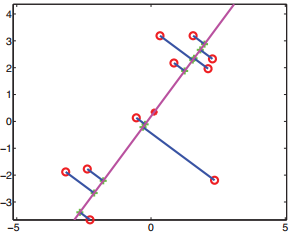
\includegraphics[scale=.60]{PCA-PPCA-a.png}} \\
\subfloat[]{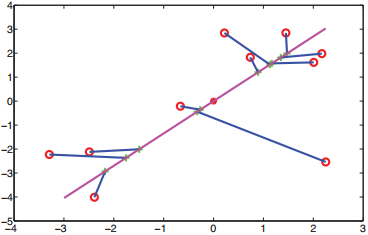
\includegraphics[scale=.60]{PCA-PPCA-b.png}}
\caption{An illustration of PCA and PPCA where $D=2$ and $L=1$. Circles are the original data points, crosses are the reconstructions. The red star is the data mean. (a) PCA. The points are orthogonally projected onto the line. (b) PPCA. The projection is no longer orthogonal: the reconstructions are shrunk towards the data mean (red star).}
\label{fig:PCA-PPCA} 
\end{figure}

The principal directions are the ones along which the data shows maximal variance. This means that PCA can be “misled” by directions in which the variance is high merely because of the measurement scale. It is therefore standard practice to standardize the data first, or equivalently, to work with correlation matrices instead of covariance matrices. 


\subsubsection{Proof *}
See Section 12.2.2 of MLAPP.


\subsection{Singular value decomposition (SVD)}
We have defined the solution to PCA in terms of eigenvectors of the covariance matrix. However, there is another way to obtain the solution, based on the \textbf{singular value decomposition}, or \textbf{SVD}. This basically generalizes the notion of eigenvectors from square matrices to any kind of matrix.

\begin{theorem}(\textbf{SVD}).
Any matrix can be decomposed as follows
\begin{equation}\label{eqn:SVD}
\underbrace{\vec{X}}_{N \times D}=\underbrace{\vec{U}}_{N \times N}\underbrace{\vec{\Sigma}}_{N \times D}\underbrace{\vec{V}^T}_{D \times D}
\end{equation}
where $\vec{U}$ is an $N \times N$ matrix whose columns are orthornormal(so $\vec{U}^T\vec{U}=\vec{I}$), $\vec{V}$ is $D \times D$ matrix whose rows and columns are orthonormal (so $\vec{V}^T\vec{V}=\vec{V}\vec{V}^T=\vec{I}_D$), and $\vec{\Sigma}$ is a $N \times D$ matrix containing the $r=\min(N,D)$ singular values $\sigma_i \geq 0$ on the main diagonal, with 0s filling the rest of the matrix.
\end{theorem}

This shows how to decompose the matrix $X$ into the product of three matrices: $\vec{V}$ describes an orthonormal basis in the domain, and $\vec{U}$ describes an orthonormal basis in the co-domain, and $\vec{\Sigma}$ describes how much the vectors in $\vec{V}$ are stretched to give the vectors in $\vec{U}$.

Since there are at most $D$ singular values (assuming $N>D$), the last $N−D$ columns of $\vec{U}$ are irrelevant, since they will be multiplied by 0. The \textbf{economy sized SVD}, or \textbf{thin SVD}, avoids computing these unnecessary elements. Let us denote this decomposition by $\hat{\vec{U}}\hat{\vec{\Sigma}}\hat{\vec{V}}^T$.If $N>D$, we have
\begin{equation}
\underbrace{\vec{X}}_{N \times D}=\underbrace{\hat{\vec{U}}}_{N \times D}\underbrace{\hat{\vec{\Sigma}}}_{D \times D}\underbrace{\hat{\vec{V}}^T}_{D \times D}
\end{equation}
as in Figure \ref{fig:SVD}(a). If $N<D$, we have
\begin{equation}
\underbrace{\vec{X}}_{N \times D}=\underbrace{\hat{\vec{U}}}_{N \times N}\underbrace{\hat{\vec{\Sigma}}}_{N \times N}\underbrace{\hat{\vec{V}}^T}_{N \times D}
\end{equation}
Computing the economy-sized SVD takes $O(ND\min(N,D))$ time (Golub and van Loan 1996, p254).

\begin{figure}[hbtp]
\centering
\subfloat[]{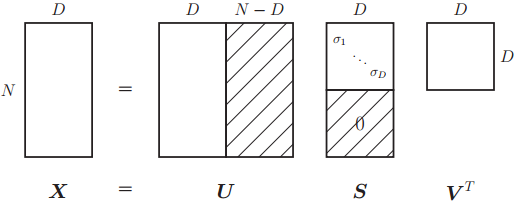
\includegraphics[scale=.50]{SVD-a.png}} \\
\subfloat[]{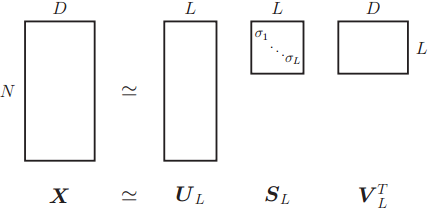
\includegraphics[scale=.50]{SVD-b.png}}
\caption{(a) SVD decomposition of non-square matrices $\vec{X}=\vec{U}\vec{\Sigma}\vec{V}^T$. The shaded parts of $\vec{\Sigma}$, and all the off-diagonal terms, are zero. The shaded entries in $\vec{U}$ and $\vec{\Sigma}$ are not computed in the economy-sized version, since they are not needed. (b) Truncated SVD approximation of rank $L$.}
\label{fig:SVD} 
\end{figure}

The connection between eigenvectors and singular vectors is the following:
\begin{align}
\vec{U}&=\mathrm{evec}(\vec{X}\vec{X}^T) \\
\vec{V}&=\mathrm{evec}(\vec{X}^T\vec{X}) \\
\vec{\Sigma}^2&=\mathrm{eval}(\vec{X}\vec{X}^T)=\mathrm{eval}(\vec{X}^T\vec{X})
\end{align}
For the proof please read Section 12.2.3 of MLAPP.

Since the eigenvectors are unaffected by linear scaling of a matrix, we see that the right singular vectors of $\vec{X}$ are equal to the eigenvectors of the empirical covariance $\hat{\vec{\Sigma}}$. Furthermore, the eigenvalues of $\hat{\vec{\Sigma}}$ are a scaled version of the squared singular values.

However, the connection between PCA and SVD goes deeper. From Equation \ref{eqn:SVD}, we can represent a rank $r$ matrix as follows:
\begin{equation*}
\vec{X}=\sigma_1\left(\begin{array}{c} | \\ \vec{u}_1 \\ | \end{array}\right)\left(\begin{array}{ccc} - & \vec{v}_1 & - \end{array}\right)+\cdots+\sigma_r\left(\begin{array}{c} | \\ \vec{u}_r \\ | \end{array}\right)\left(\begin{array}{ccc} - & \vec{v}_r^T & - \end{array}\right)
\end{equation*}
If the singular values die off quickly, we can produce a rank $L$ approximation to the matrix as follows:
\begin{align}
\vec{X} & \approx \sigma_1\left(\begin{array}{c} | \\ \vec{u}_1 \\ | \end{array}\right)\left(\begin{array}{ccc} - & \vec{v}_1 & - \end{array}\right)+\cdots+\sigma_r\left(\begin{array}{c} | \\ \vec{u}_L \\ | \end{array}\right)\left(\begin{array}{ccc} - & \vec{v}_L^T & - \end{array}\right) \nonumber \\
 & = \vec{U}_{:,1:L}\vec{\Sigma}_{1:L,1:L}\vec{V}_{:,1:L}^T
\end{align}
This is called a \textbf{truncated SVD} (see Figure \ref{fig:SVD}(b)).

One can show that the error in this approximation is given by
\begin{equation}
\lVert \vec{X}-\vec{X}_L \rVert_F \approx \sigma_L
\end{equation}
Furthermore, one can show that the SVD offers the best rank $L$ approximation to a matrix (best in the sense of minimizing the above Frobenius norm).

Let us connect this back to PCA. Let $\vec{X}=\vec{U}\vec{\Sigma}\vec{V}^T$ be a truncated SVD of $\vec{X}$. We know that $\hat{\vec{W}}=\vec{V}$, and that $\hat{\vec{Z}}=\vec{X}\hat{\vec{W}}$, so
\begin{equation}
\hat{\vec{Z}}=\vec{U}\vec{\Sigma}\vec{V}^T\vec{V}=\vec{U}\vec{\Sigma}
\end{equation}
Furthermore, the optimal reconstruction is given by $\hat{\vec{X}}=\vec{Z}\hat{\vec{W}}$,so we find
\begin{equation}
\hat{\vec{X}}=\vec{U}\vec{\Sigma}\vec{V}^T
\end{equation}
This is precisely the same as a truncated SVD approximation! This is another illustration of the fact that PCA is the best low rank approximation to the data.


\subsection{Probabilistic PCA}
\begin{theorem}((\textbf{Tipping and Bishop 1999})).
Consider a factor analysis model in which $\vec{\Psi}=\sigma^2\vec{I}$ and $\vec{W}$ is orthogonal. The observed data log likelihood is given by
\begin{align}
\log p(\vec{X}|\vec{W},\sigma^2\vec{I}) & =-\frac{N}{2}\ln|\vec{C}|-\frac{1}{2}\sum\limits_{i=1}^N \vec{x}_i^T\vec{C}^{-1}\vec{x}_i \nonumber \\
   & =-\frac{N}{2}\ln|\vec{C}|+\mathrm{tr}(\vec{C}^{-1}\vec{\Sigma})
\end{align}
where $\vec{C}=\vec{W}\vec{W}^T+\sigma^2\vec{I}$ and $\vec{\Sigma}=\frac{1}{N}\sum_{i=1}^N \vec{x}_i\vec{x}_i^T=\frac{1}{N}\vec{X}\vec{X}^T$. (We are assuming centred data, for notational simplicity.) The maxima of the log-likelihood are given by
\begin{equation}
\hat{\vec{W}}=\vec{V}(\vec{\Lambda}-\sigma^2\vec{I})^{\frac{1}{2}}\vec{R}
\end{equation}
where $\vec{R}$ is an arbitrary $L \times L$ orthogonal matrix, $\vec{V}$ is the $D \times L$ matrix whose columns are the first $L$ eigenvectors of $\vec{\Sigma}$, and $\vec{\Lambda}$ is the corresponding diagonal matrix of eigenvalues. Without loss of generality, we can set $\vec{R}=\vec{I}$. Furthermore, the MLE of the noise variance is given by
\begin{equation}
\hat{\sigma}^2=\frac{1}{D-L}\sum\limits_{j=L+1}^D \lambda_j
\end{equation}
which is the average variance associated with the discarded dimensions.
\end{theorem}

Thus, as $\sigma^2 \rightarrow 0$, we have $\hat{\vec{W}} \rightarrow \vec{V}$, as in classical PCA. What about $\hat{\vec{Z}}$? It is easy to see that the posterior over the latent factors is given by
\begin{align}
p(\vec{z}_i|\vec{x}_i,\hat{\vec{\theta}}) & = \mathcal{N}(\vec{z}_i|\hat{\vec{F}}^{-1}\hat{\vec{W}}^T\vec{x}_i,\sigma^2\hat{\vec{F}}^{-1}) \label{eqn:PPCA-posterior}\\
\hat{\vec{F}} & \triangleq \hat{\vec{W}}^T\hat{\vec{W}}+\sigma^2\vec{I}
\end{align}
(Do not confuse $\vec{F} = \vec{W}^T\vec{W}+\sigma^2\vec{I}$ with $\vec{C}=\vec{W}\vec{W}^T+\sigma^2\vec{I}$.) Hence, as $\sigma^2 \rightarrow 0$, we find $\hat{\vec{W}} \rightarrow \vec{V}$, $\hat{\vec{F}} \rightarrow \vec{I}$ and $\vec{z}_i \rightarrow \vec{V}^T\vec{x}_i$. Thus the posterior mean is obtained by an orthogonal projection of the data onto the column space of $\vec{V}$, as in classical PCA.

Note, however, that if $\sigma^2 \rightarrow 0$, the posterior mean is not an orthogonal projection, since it is shrunk somewhat towards the prior mean, as illustrated in Figure \ref{fig:PCA-PPCA}(b). This sounds like an undesirable property, but it means that the reconstructions will be closer to the overall data mean, $\hat{\vec{\mu}}=\bar{\vec{x}}$.


\subsection{EM algorithm for PCA}
\label{sec:EM-for-PCA}
Although the usual way to fit a PCA model uses eigenvector methods, or the SVD, we can also use EM, which will turn out to have some advantages that we discuss below. EM for PCA relies on the probabilistic formulation of PCA. However the algorithm continues to work in the zero noise limit, $\sigma^2=0$, as shown by (Roweis 1997).

Let $\tilde{\vec{Z}}$ be a $L \times N$ matrix storing the posterior means (low-dimensional representations) along its columns. Similarly, let $\tilde{\vec{X}}=\vec{X}^T$ store the original data along its columns. From Equation \ref{eqn:PPCA-posterior}, when $\sigma^2=0$, we have
\begin{equation}
\tilde{\vec{Z}}=(\vec{W}^T\vec{W})^{-1}\vec{W}^T\tilde{\vec{X}}
\end{equation}
This constitutes the E step. Notice that this is just an orthogonal projection of the data.

From Equation \ref{eqn:FA-EM-W}, the M step is given by
\begin{equation}
\hat{\vec{W}}=\left(\sum\limits_{i=1}^N \vec{x}_i\mathbb{E}[\vec{z}_i]^T\right)\left(\sum\limits_{i=1}^N \mathbb{E}[\vec{z}_i]\mathbb{E}[\vec{z}_i]^T\right)^{-1}
\end{equation}
where we exploited the fact that $\vec{\Sigma}=\mathrm{cov}[\vec{z}_i|\vec{x}_i,\vec{\theta}]=\vec{0}$ when $\sigma^2=0$.

(Tipping and Bishop 1999) showed that the only stable fixed point of the EM algorithm is the globally optimal solution. That is, the EM algorithm converges to a solution where $\vec{W}$ spans the same linear subspace as that defined by the first $L$ eigenvectors. However, if we want $\vec{W}$ to be orthogonal, and to contain the eigenvectors in descending order of eigenvalue, we have to orthogonalize the resulting matrix (which can be done quite cheaply). Alternatively, we can modify EM to give the principal basis directly (Ahn and Oh 2003).

This algorithm has a simple physical analogy in the case $D=2$ and $L=1$(Roweis 1997). Consider some points in $\mathbb{R}^2$ attached by springs to a rigid rod, whose orientation is defined by a vector $\vec{w}$. Let $\vec{z}_i$ be the location where the $i$'th spring attaches to the rod. See Figure 12.11 of MLAPP for an illustration.

Apart from this pleasing intuitive interpretation, EM for PCA has the following advantages over eigenvector methods:
\begin{itemize}
\item{EM can be faster. In particular, assuming $N,D \gg L$, the dominant cost of EM is the projection operation in the E step, so the overall time is $O(TLND)$, where $T$ is the number of iterations. This is much faster than the $O(\min(ND^2,DN^2))$ time required by straightforward eigenvector methods, although more sophisticated eigenvector methods, such as the Lanczos algorithm, have running times comparable to EM.}
\item{EM can be implemented in an online fashion, i.e., we can update our estimate of $\vec{W}$ as the data streams in.}
\item{EM can handle missing data in a simple way (see Section \ref{sec:Fitting-FA-models-with-missing-data}).}
\item{EM can be extended to handle mixtures of PPCA/ FA models.}
\item{EM can be modified to variational EM or to variational Bayes EM to fit more complex models.}
\end{itemize}


\section{Choosing the number of latent dimensions}
\label{sec:FA-Choosing-L}
In Section \ref{sec:Model-selection-for-LVM}, we discussed how to choose the number of components $K$ in a mixture model. In this section, we discuss how to choose the number of latent dimensions $L$ in a FA/PCA model.


\subsection{Model selection for FA/PPCA}
TODO

\subsection{Model selection for PCA}
TODO



\section{PCA for categorical data}
In this section, we consider extending the factor analysis model to the case where the observed data is categorical rather than real-valued. That is, the data has the form $y_{ij} \in \{1,...,C\}$, where $j=1:R$ is the number of observed response variables. We assume each $y_{ij}$ is generated from a latent variable $\vec{z}_i \in \mathbb{R}^L$, with a Gaussian prior, which is passed through the softmax function as follows:
\begin{align}
p(\vec{z}_i) & = \mathcal{N}(\vec{z}_i|\vec{0},\vec{I}) \\
p(\vec{y}_i|\vec{z}_i,\vec{\theta}) & = \prod\limits_{j=1}^R \mathrm{Cat}(y_{ir}|\mathcal{S}(\vec{W}_r^T\vec{z}_i+\vec{w}_{0r}))
\end{align}
where $\vec{W}_r \in \mathbb{R}^L$ is the factor loading matrix for response $j$, and $\vec{W}_{0r} \in \mathbb{R}^M$ is the offset term for response $r$, and $\vec{\theta}=(\vec{W}_r,\vec{W}_{0r})_{r=1}^R$. (We need an explicit offset term, since clamping one element of $\vec{z}_i$ to 1 can cause problems when computing the posterior covariance.) As in factor analysis, we have defined the prior mean to be $\vec{\mu}_0=\vec{0}$ and the prior covariance $\vec{V}_0=\vec{I}$, since we can capture non-zero mean by changing $\vec{w}_{0j}$ and non-identity covariance by changing $\vec{W}_r$. We will call this categorical PCA. See Chapter 27 TODO for a discussion of related models.

In (Khan et al. 2010), we show that this model outperforms finite mixture models on the task of imputing missing entries in design matrices consisting of real and categorical data. This is useful for analysing social science survey data, which often has missing data and variables of mixed type.


\section{PCA for paired and multi-view data}


\subsection{Supervised PCA (latent factor regression)}


\subsection{Discriminative supervised PCA}


\subsection{Canonical correlation analysis}


\section{Independent Component Analysis (ICA)}
\label{sec:ICA}
Let $\vec{x}_t \in \mathbb{R}^D$ be the observed signal at the sensors at “time” $t$, and $\vec{z}_t \in \mathbb{R}^L$ be the vector of source signals. We assume that
\begin{equation}
\vec{x}_t=\vec{W}\vec{z}_t+\vec{\epsilon}_t
\end{equation}
where $\vec{W}$ is an $D \times L$ matrix, and $\vec{\epsilon}_t \sim \mathcal{N}(\vec{0},\vec{\Psi})$. In this section, we treat each time point as an independent observation, i.e., we do not model temporal correlation (so we could replace the $t$ index with $i$, but we stick with t to be consistent with much of the ICA literature). The goal is to infer the source signals, $p(\vec{z}_t|\vec{x}_t,\vec{\theta})$. In this context, $\vec{W}$ is called the \textbf{mixing matrix}. If $L=D$ (number of sources = number of sensors), it will be a square matrix. Often we will assume the noise level, $|\vec{\Psi}|$, is zero, for simplicity.

So far, the model is identical to factor analysis. However, we will use a different prior for $p(\vec{z}_t)$. In PCA, we assume each source is independent, and has a Gaussian distribution. We will now relax this Gaussian assumption and let the source distributions be any \emph{non-Gaussian} distribution
\begin{equation}
p(\vec{z}_t) =\prod\limits_{j=1}^L p_j(z_{tj})
\end{equation}
Without loss of generality, we can constrain the variance of the source distributions to be \vec{1}, because any other variance can be modelled by scaling the rows of $\vec{W}$ appropriately. The resulting model is known as \textbf{independent component analysis} or \textbf{ICA}.

The reason the Gaussian distribution is disallowed as a source prior in ICA is that it does not permit unique recovery of the sources. This is because the PCA likelihood is invariant to any orthogonal transformation of the sources $\vec{z}_t$ and mixing matrix $\vec{W}$. PCA can recover the best linear subspace in which the signals lie, but cannot uniquely recover the signals themselves.

ICA requires that $\vec{W}$ is square and hence invertible. In the non-square case (e.g., where we have more sources than sensors), we cannot uniquely recover the true signal, but we can compute the posterior $p(\vec{z}_t|\vec{x}_t,\hat{\vec{W}})$, which represents our beliefs about the source. In both cases, we need to estimate Was well as the source distributions $p_j$. We discuss how to do this below.


\subsection{Maximum likelihood estimation}
In this section, we discuss ways to estimate square mixing matrices $\vec{W}$ for the noise-free ICA model. As usual, we will assume that the observations have been centered; hence we can also assume $\vec{z}$ is zero-mean. In addition, we assume the observations have been whitened, which can be done with PCA. 

If the data is centered and whitened, we have $\mathbb{E}[\vec{x}\vec{x}^T]=\vec{I}$. But in the noise free case, we also have
\begin{equation}
\mathrm{cov}[\vec{x}]=\mathbb{E}[\vec{x}\vec{x}^T]=\vec{W}\mathbb{E}[\vec{z}\vec{z}^T]\vec{W}^T
\end{equation}
Hence we see that $\vec{W}$ must be orthogonal. This reduces the number of parameters we have to estimate from $D^2$ to $D(D-1)/2$. It will also simplify the math and the algorithms.

Let $\vec{V}=\vec{W}^{-1}$; these are often called the recognition weights, as opposed to $\vec{W}$, which are the generative weights.

Since $\vec{x}=\vec{W}\vec{z}$, we have, from Equation \ref{eqn:Multivariate-transformation},
\begin{align}
p_x(\vec{W}\vec{z}_t) & =p_z(\vec{z}_t)|\mathrm{det}(\vec{W}^{-1})| \nonumber \\
   & = p_z(\vec{V}\vec{x}_t)|\mathrm{det}(\vec{V})|
\end{align}
Hence we can write the log-likelihood, assuming $T$ iid samples, as follows:
\begin{equation*}
\frac{1}{T} \log p(\mathcal{D}|\vec{V})=\log|\mathrm{det}(\vec{V})|+\frac{1}{T}\sum\limits_{j=1}^L \sum\limits_{t=1}^T \log p_j(\vec{v}_j^T\vec{x}_t)
\end{equation*}
where $\vec{v}_j$ is the $j$'th row of $\vec{V}$. Since we are constraining $\vec{V}$ to be orthogonal, the first term is a constant, so we can drop it. We can also replace the average over the data with an expectation operator to get the following objective
\begin{equation}
\mathrm{NLL}(\vec{V})=\sum\limits_{j=1}^L \mathbb{E}[G_j(\vec{z}_j)]
\end{equation}
where $\vec{z}_j=\vec{v}_j^T\vec{x}$ and $G_j(\vec{z}) \triangleq -\log p_j(\vec{z})$. We want to minimize this subject to the constraint that the rows of $\vec{V}$ are orthogonal. We also want them to be unit norm, since this ensures that the variance of the factors is unity (since, with whitened data, $\mathbb{E}[\vec{v}_j^T\vec{x}]=\lVert \vec{v}_j \rVert^2$, which is necessary to fix the scale of the weights. In otherwords, $\vec{V}$ should be an orthonormal matrix.

It is straightforward to derive a gradient descent algorithm to fit this model; however, it is rather slow. One can also derive a faster algorithm that follows the natural gradient; see e.g., (MacKay 2003, ch 34) for details. A popular alternative is to use an approximate Newton method, which we discuss in Section \ref{sec:FastICA}. Another approach is to use EM, which we discuss in Section \ref{sec:ICA-EM}.


\subsection{The FastICA algorithm}
\label{sec:FastICA}


\subsection{Using EM}
\label{sec:ICA-EM}


\subsection{Other estimation principles *}


\chapter{Sparse linear models}


\chapter{Kernels}
\label{chap:Kernels}

\section{Introduction}
So far in this book, we have been assuming that each object that we wish to classify or cluster or process in anyway can be represented as a fixed-size feature vector, typically of the form $\vec{x}_i \in \mathbb{R}^D$. However, for certain kinds of objects, it is not clear how to best represent them as fixed-sized feature vectors. For example, how do we represent a text document or protein sequence, which can be of variable length? or a molecular structure, which has complex 3d geometry? or an evolutionary tree, which has variable size and shape?

One approach to such problems is to define a generative model for the data, and use the inferred latent representation and/or the parameters of the model as features, and then to plug these features in to standard methods. For example, in Chapter 28 TODO, we discuss deep learning, which is essentially an unsupervised way to learn good feature representations.

Another approach is to assume that we have some way of measuring the similarity between objects, that doesn’t require preprocessing them into feature vector format. For example, when comparing strings, we can compute the edit distance between them. Let $\kappa(\vec{x},\vec{x}') \geq 0$ be some measure of similarity between objects $\kappa(\vec{x},\vec{x}') \in \mathcal{X}$,  we will call $\kappa$ a \textbf{kernel function}. Note that the word “kernel” has several meanings; we will discuss a different interpretation in Section 14.7.1 TODO.

In this chapter, we will discuss several kinds of kernel functions. We then describe some algorithms that can be written purely in terms of kernel function computations. Such methods can be used when we don’t have access to (or choose not to look at) the “inside” of the objects $\vec{x}$ that we are processing.


\section{Kernel functions}
\begin{definition}
A \textbf{kernel function}\footnote{\url{http://en.wikipedia.org/wiki/Kernel_function}} is a real-valued function of two arguments, $\kappa(\vec{x},\vec{x}') \in \mathbb{R}$. Typically the function is symmetric (i.e., $\kappa(\vec{x},\vec{x}')=\kappa(\vec{x}',\vec{x})$, and non-negative (i.e., $\kappa(\vec{x},\vec{x}') \geq 0$). 
\end{definition}

We give several examples below.

\subsection{RBF kernels}
The \textbf{Gaussian kernel} or \textbf{squared exponential kernel}(SE kernel) is defined by
\begin{equation}
\kappa(\vec{x},\vec{x}')=\exp\left(-\frac{1}{2}(\vec{x}-\vec{x}')^T\vec{\Sigma}^{-1}(\vec{x}-\vec{x}')\right)
\end{equation}

If $\vec{\Sigma}$ is diagonal, this can be written as
\begin{equation}
\kappa(\vec{x},\vec{x}')=\exp\left(-\frac{1}{2}\sum\limits_{j=1}^D \frac{1}{\sigma_j^2}(x_j-x_j')^2\right)
\end{equation}

We can interpret the $\sigma_j$ as defining the \textbf{characteristic length scale} of dimension $j$.If $\sigma_j = \infty$, the corresponding dimension is ignored; hence this is known as the \textbf{ARD kernel}. If $\vec{\Sigma}$ is spherical, we get the isotropic kernel
\begin{equation}\label{eqn:RBF-kernel}
\kappa(\vec{x},\vec{x}')=\exp\left(-\frac{\lVert\vec{x}-\vec{x}'\rVert^2}{2\sigma^2}\right)
\end{equation}

Here $\sigma^2$ is known as the \textbf{bandwidth}. Equation ~\ref{eqn:RBF-kernel} is an example of a \textbf{radial basis function} or \textbf{RBF} kernel, since it is only a function of $\lVert\vec{x}-\vec{x}'\rVert^2$.


\subsection{TF-IDF kernels}
\begin{equation}\label{eqn:RBF-kernel}
\kappa(\vec{x},\vec{x}')=\frac{\phi(\vec{x})^T\phi(\vec{x}')}{\lVert\phi(vec{x})\rVert_2\lVert\phi(\vec{x}')\rVert_2}
\end{equation}
where $\phi(\vec{x})=\text{tf-idf}(\vec{x})$.

\subsection{Mercer (positive definite) kernels}
\label{sec:Mercer-kernels}
If the kernel function satisfies the requirement that the \textbf{Gram matrix}, defined by
\begin{equation}
\vec{K} \triangleq \left(\begin{array}{ccc}
\kappa(\vec{x}_1,\vec{x}_2) & \cdots \kappa(\vec{x}_1,\vec{x}_N) \\
\vdots & \vdots & \vdots \\
\kappa(\vec{x}_N,\vec{x}_1) & \cdots \kappa(\vec{x}_N,\vec{x}_N) 
\end{array}\right)
\end{equation}
be positive definite for any set of inputs $\{\vec{x}_i\}_{i=1}^N$. We call such a kernel a \textbf{Mercer kernel},or \textbf{positive definite kernel}.

If the Gram matrix is positive definite, we can compute an eigenvector decomposition of it as follows
\begin{equation}
\vec{K}=\vec{U}^T\vec{\Lambda}\vec{U}
\end{equation}

where $\vec{\Lambda}$ is a diagonal matrix of eigenvalues $\lambda_i >0$. Now consider an element of $\vec{K}$:
\begin{equation}
k_{ij}=(\vec{\Lambda}^{\frac{1}{2}}\vec{U}_{:,i})^T(\vec{\Lambda}^{\frac{1}{2}}\vec{U}_{:,j})
\end{equation}

Let us define $\phi(\vec{x}_i)=\vec{\Lambda}^{\frac{1}{2}}\vec{U}_{:,i}$, then we can write
\begin{equation}
k_{ij}=\phi(\vec{x}_i)^T\phi(\vec{x}_j)
\end{equation}

Thus we see that the entries in the kernel matrix can be computed by performing an inner product of some feature vectors that are implicitly defined by the eigenvectors $\vec{U}$. In general, if the kernel is Mercer, then there exists a function $\phi$ mapping $\vec{x} \in \mathcal{X}$ to $\mathbb{R}^D$ such that
\begin{equation}
\kappa(\vec{x},\vec{x}')=\phi(\vec{x})^T\phi(\vec{x}')
\end{equation}
where $\phi$ depends on the eigen functions of $\kappa$(so $D$ is a potentially infinite dimensional space).

For example, consider the (non-stationary) \textbf{polynomial kernel} $\kappa(\vec{x},\vec{x}')=(\gamma \vec{x}\vec{x}'+r)^M$, where $r>0$. One can show that the corresponding feature vector $\phi(\vec{x})$ will contain all terms up to degree $M$. For example, if $M=2, \gamma=r=1$ and $\vec{x}, \vec{x}' \in \mathbb{R}^2$, we have
\begin{align*}
(\vec{x}\vec{x}'+1)^2 & =(1+x_1x_1'+x_2+x_2')^2 \\
    & = 1+2x_1x_1'+2x_2x_2'+(x_1x_1')^2+(x_2x_2')^2x_1x_1'x_2x_2' \\
	& = \phi(\vec{x})^T\phi(\vec{x}') \\
\text{where } & \phi(\vec{x})=(1,\sqrt{2}x_1,\sqrt{2}x_2,x_1^2,x_2^2,\sqrt{2}x_1x_2)
\end{align*}

In the case of a Gaussian kernel, the feature map lives in an infinite dimensional space. In such a case, it is clearly infeasible to explicitly represent the feature vectors.

In general, establishing that a kernel is a Mercer kernel is difficult, and requires techniques from functional analysis. However, one can show that it is possible to build up new Mercer kernels from simpler ones using a set of standard rules. For example, if $\kappa_1$ and $\kappa_2$ are both Mercer, so is $\kappa(\vec{x},\vec{x}')=\kappa_1(\vec{x},\vec{x}')+\kappa_2(\vec{x},\vec{x}')=$. See e.g., (Schoelkopf and Smola 2002) for details.


\subsection{Linear kernels}
\begin{equation}
\kappa(\vec{x},\vec{x}')=\vec{x}^T\vec{x}'
\end{equation}

\subsection{Matern kernels}
The \textbf{Matern kernel}, which is commonly used in Gaussian process regression (see Section 15.2), has the following form
\begin{equation}
\kappa(r)=\frac{2^{1-\nu}}{\Gamma(\nu)}\left(\frac{\sqrt{2\nu}r}{\ell}\right)^{\nu}K_{\nu}\frac{\sqrt{2\nu}r}{\ell}
\end{equation}
where $r=\lVert\vec{x}-\vec{x}'\rVert$, $\nu>0$, $\ell>0$, and $K_{\nu}$ is a modified Bessel function. As $\nu \rightarrow \infty$, this approaches the SE kernel. If $\nu=\frac{1}{2}$, the kernel simplifies to
\begin{equation}
\kappa(r)=\exp(-r/\ell)
\end{equation}

If $D=1$, and we use this kernel to define a Gaussian process (see Chapter 15 TODO), we get the \textbf{Ornstein-Uhlenbeck process}, which describes the velocity of a particle undergoing Brownian motion (the corresponding function is continuous but not differentiable, and hence is very “jagged”).


\subsection{String kernels}
\label{sec:String-kernels}
Now let $\phi_s(\vec{x})$ denote the number of times that substrings appears in string $\vec{x}$. We define the kernel between two strings $\vec{x}$ and $\vec{x}'$ as
\begin{equation}
\kappa(\vec{x},\vec{x}')=\sum\limits_{s \in \mathcal{A}^*} w_s\phi_s(\vec{x})\phi_s(\vec{x}')
\end{equation}
where $w_s \geq 0$ and $\mathcal{A}^*$ is the set of all strings (of any length) from the alphabet $\mathcal{A}$(this is known as the Kleene star operator). This is a Mercer kernel, and be computed in $O(|\vec{x}|+|\vec{x}'|)$ time (for certain settings of the weights $\{ws\}$) using suffix trees (Leslie et al. 2003; Vishwanathan and Smola 2003; Shawe-Taylor and Cristianini 2004).

There are various cases of interest. If we set $w_s =0$for $|s| >1$ we get a bag-of-characters kernel. This defines $\phi(\vec{x})$ to be the number of times each character in $\mathcal{A}$ occurs in $\vec{x}$.If we require $s$ to be bordered by white-space, we get a bag-of-words kernel, where $\phi(\vec{x})$ counts how many times each possible word occurs. Note that this is a very sparse vector, since most words will not be present. If we only consider strings of a fixed lengthk, we get the \textbf{k-spectrum} kernel. This has been used to classify proteins into SCOP superfamilies (Leslie et al. 2003).


\subsection{Pyramid match kernels}
% \begin{figure}[hbtp]
% \centering
%     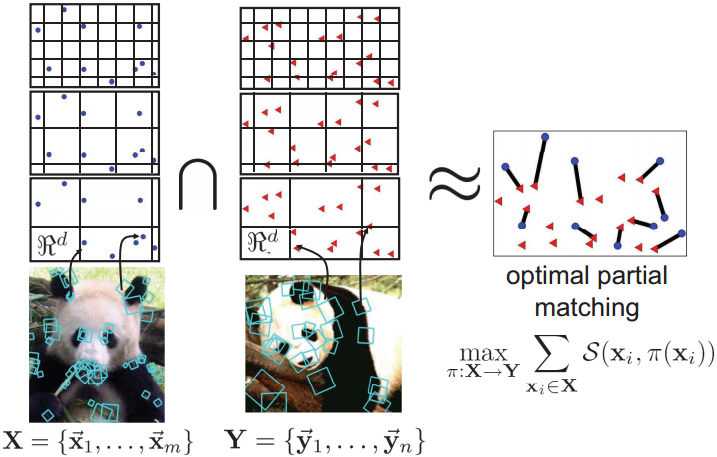
\includegraphics[scale=.70]{pyramid-match-kernel.png}
% \caption{Illustration of a pyramid match kernel computed from two images. Used with kind permission of Kristen Grauman.}
% \label{fig:pyramid-match-kernel}
% \end{figure}


\subsection{Kernels derived from probabilistic generative models}
Suppose we have a probabilistic generative model of feature vectors, $p(\vec{x}|\vec{\theta})$. Then there are several ways we can use this model to define kernel functions, and thereby make the model suitable for discriminative tasks. We sketch two approaches below.


\subsubsection{Probability product kernels}
\begin{equation}\label{eqn:Probability-product-kernels}
\kappa(\vec{x}_i,\vec{x}_j)=\int p(\vec{x}|\vec{x}_i)^{\rho}p(\vec{x}|\vec{x}_j)^{\rho}\mathrm{d}\vec{x}
\end{equation}
where $\rho>0$, and $p(\vec{x}|\vec{x}_i)$ is often approximated by $p(\vec{x}|\hat{\vec{\theta}}(\vec{x}_i))$,where $\hat{\vec{\theta}}(\vec{x}_i)$ is a parameter estimate computed using a single data vector. This is called a \textbf{probability product kernel}(Jebara et al. 2004).

Although it seems strange to fit a model to a single data point, it is important to bear in mind that the fitted model is only being used to see how similar two objects are. In particular, if we fit the model to $\vec{x}_i$ and then the model thinks $\vec{x}_j$ is likely, this means that $\vec{x}_i$ and $\vec{x}_j$ are similar. For example, suppose $p(\vec{x}|\vec{\theta}) \sim \mathcal{N}(\vec{\mu},\sigma^2\vec{I})$, where $\sigma^2$ is fixed. If $\rho=1$, and we use $\hat{\vec{\mu}}(\vec{x}_i)=\vec{x}_i$ and $\hat{\vec{\mu}}(\vec{x}_j)=\vec{x}_j$, we find (Jebara et al. 2004, p825) that
\begin{equation}
\kappa(\vec{x}_i,\vec{x}_j)=\frac{1}{(4\pi\sigma^2)^{D/2}}\exp\left(-\frac{1}{4\sigma^2}\lVert\vec{x}_i-\vec{x}_j\rVert^2\right)
\end{equation}
which is (up to a constant factor) the RBF kernel.

It turns out that one can compute Equation ~\ref{eqn:Probability-product-kernels} for a variety of generative models, including ones with latent variables, such as HMMs. This provides one way to define kernels on variable length sequences. Furthermore, this technique works even if the sequences are of real-valued vectors, unlike the string kernel in Section \ref{sec:String-kernels}. See (Jebara et al. 2004) for further details


\subsubsection{Fisher kernels}
A more efficient way to use generative models to define kernels is to use a \textbf{Fisher kernel} (Jaakkola and Haussler 1998) which is defined as follows:
\begin{equation}
\kappa(\vec{x}_i,\vec{x}_j)=g(\vec{x}_i)^T\vec{F}^{-1}g(\vec{x}_j)
\end{equation}
where $g$ is the gradient of the log likelihood, or \textbf{score vector}, evaluated at the MLE $\hat{\vec{\theta}}$
\begin{equation}
g(\vec{x}) \triangleq \frac{\mathrm{d}}{\mathrm{d}\vec{\theta}}\log p(\vec{x}|\vec{\theta})|_{\hat{\vec{\theta}}}
\end{equation}
and $\vec{F}$ is the Fisher information matrix, which is essentially the Hessian:
\begin{equation}
\vec{F} \triangleq \left[\frac{\partial^2}{\partial \theta_i \partial \theta_j}\log p(\vec{x}|\vec{\theta})\right]|_{\hat{\vec{\theta}}}
\end{equation}

Note that $\hat{\vec{\theta}}$ is a function of all the data, so the similarity of $\vec{x}_i$ and $\vec{x}_j$ is computed in the context of all the data as well. Also, note that we only have to fit one model.


\section{Using kernels inside GLMs}


\subsection{Kernel machines}
We define a \textbf{kernel machine} to be a GLM where the input feature vector has the form
\begin{equation}\label{eqn:kernel-machine}
\phi(\vec{x})=(\kappa(\vec{x},\vec{\mu}_1),\cdots,\kappa(\vec{x},\vec{\mu}_K))
\end{equation}

where $\vec{\mu}_k \in \mathcal{X}$ are a set of $K$ centroids. If $\kappa$ is an RBF kernel, this is called an \textbf{RBF network}. We discuss ways to choose the $\vec{\mu}_k$ parameters below. We will call Equation \ref{eqn:kernel-machine} a \textbf{kernelised feature vector}. Note that in this approach, the kernel need not be a Mercer kernel.

We can use the kernelized feature vector for logistic regression by defining $p(y|\vec{x},\vec{\theta})=\mathrm{Ber}(y|\vec{w}^T\phi(\vec{x}))$. This provides a simple way to define a non-linear decision boundary. For example, see Figure \ref{fig:kenel-machine-xor}.

\begin{figure}[hbtp]
\centering
\subfloat[]{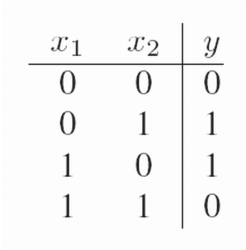
\includegraphics[scale=.70]{kenel-machine-xor-a.png}} \\
\subfloat[]{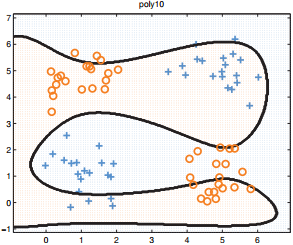
\includegraphics[scale=.70]{kenel-machine-xor-b.png}} \\
\subfloat[]{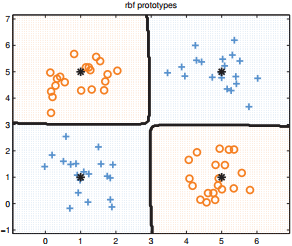
\includegraphics[scale=.70]{kenel-machine-xor-c.png}}
\caption{(a) xor truth table. (b) Fitting a linear logistic regression classifier using degree 10 polynomial expansion. (c) Same model, but using an RBF kernel with centroids specified by the 4 black crosses.}
\label{fig:kenel-machine-xor} 
\end{figure}

We can also use the kernelized feature vector inside a linear regression model by defining $p(y|\vec{x},\vec{\theta})=\mathcal{N}(y|\vec{w}^T\phi(\vec{x}),\sigma^2)$. 


\subsection{L1VMs, RVMs, and other sparse vector machines}
\label{sec:sparse-kernel-machines}
The main issue with kernel machines is: how do we choose the centroids $\vec{\mu}_k$? We can use \textbf{sparse vector machine}, \textbf{L1VM}, \textbf{L2VM}, \textbf{RVM}, \textbf{SVM}.

% In Figure \ref{fig:L2VM-L1VM-RVM-SVM-2d}, we compare L2VM, L1VM, RVM and an SVM using the same RBF kernel on a binary classification problem in 2d.

% \begin{figure}[hbtp]
% \centering
% \subfloat[]{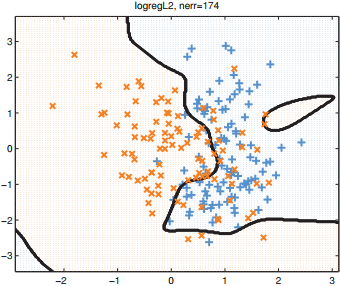
\includegraphics[scale=.50]{L2VM-L1VM-RVM-SVM-2d-a.png}} \\
% \subfloat[]{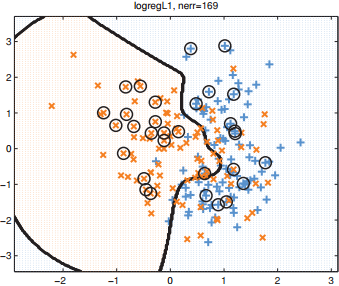
\includegraphics[scale=.50]{L2VM-L1VM-RVM-SVM-2d-b.png}} \\
% \subfloat[]{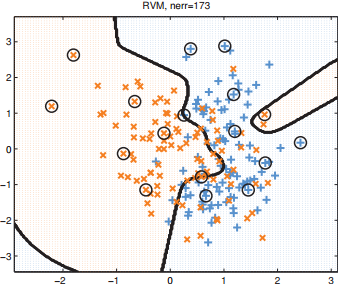
\includegraphics[scale=.50]{L2VM-L1VM-RVM-SVM-2d-c.png}} \\
% \subfloat[]{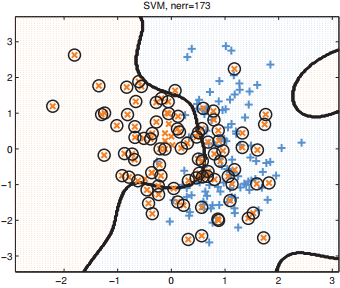
\includegraphics[scale=.50]{L2VM-L1VM-RVM-SVM-2d-d.png}}
% \caption{Example of non-linear binary classification using an RBF kernel with bandwidth $\sigma=0.3$. (a) L2VM with $\lambda=5$. (b) L1VM with $\lambda=1$. (c) RVM. (d) SVM with $C=1/\lambda$ chosen by cross validation. Black circles denote the support vectors.}
% \label{fig:L2VM-L1VM-RVM-SVM-2d} 
% \end{figure}

% In Figure \ref{fig:L2VM-L1VM-RVM-SVM-1d}, we compare L2VM, L1VM, RVM and an SVM using an RBF kernel on a 1d regression problem. 
% \begin{figure}[hbtp]
% \centering
%     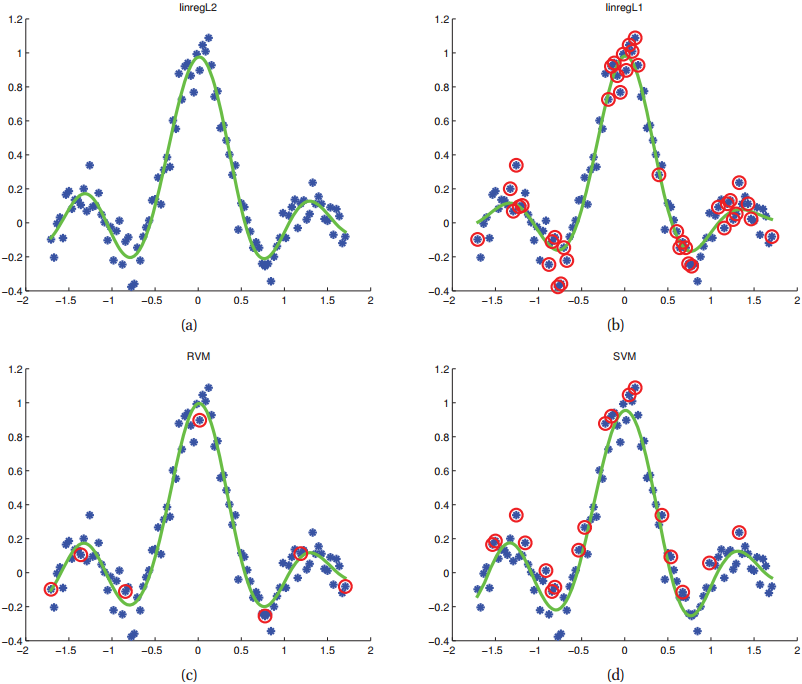
\includegraphics[scale=.70]{L2VM-L1VM-RVM-SVM-1d.png}
% \caption{Example of kernel based regression on the noisy sinc function using an RBF kernel with bandwidth $\sigma=0.3$. (a) L2VM with $\lambda=0.5$. (b) L1VM with $\lambda=0.5$. (c) RVM. (d) SVM regression with $C=1/\lambda$ chosen by cross validation, and $\epsilon=0.1$ (the default for SVMlight). Red circles denote the retained training exemplars.}
% \label{fig:L2VM-L1VM-RVM-SVM-1d} 
% \end{figure}


\section{The kernel trick}
Rather than defining our feature vector in terms of kernels, $\phi(\vec{x})=(\kappa(\vec{x},\vec{x}_1),\cdots,\kappa(\vec{x},\vec{x}_N))$, we can instead work with the original feature vectors $\vec{x}$, but modify the algorithm so that it replaces all inner products of the form $<\vec{x}_i,\vec{x}_j>$ with a call to the kernel function, $\kappa(\vec{x}_i,\vec{x}_j)$. This is called the \textbf{kernel trick}. It turns out that many algorithms can be kernelized in this way. We give some examples below. Note that we require that the kernel be a Mercer kernel for this trick to work.


\subsection{Kernelized KNN}
The Euclidean distance can be unrolled as
\begin{equation}\label{eqn:Euclidean-distance}
\lVert\vec{x}_i-\vec{x}_j\rVert=<\vec{x}_i,\vec{x}_i>+<\vec{x}_j,\vec{x}_j>-2<\vec{x}_i,\vec{x}_j>
\end{equation}
then by replacing all $<\vec{x}_i,\vec{x}_j>$ with $\kappa(\vec{x}_i,\vec{x}_j)$ we get Kernelized KNN.


\subsection{Kernelized K-medoids clustering}
\textbf{K-medoids algorothm} is similar to K-means(see Section \ref{sec:K-means}), but instead of representing each cluster’s centroid by the mean of all data vectors assigned to this cluster, we make each centroid be one of the data vectors themselves. Thus we always deal with integer indexes, rather than data objects.

This algorithm can be kernelized by using Equation \ref{eqn:Euclidean-distance} to replace the distance computation.


\subsection{Kernelized ridge regression}
Applying the kernel trick to distance-based methods was straightforward. It is not so obvious how to apply it to parametric models such as ridge regression. However, it can be done, as we now explain. This will serve as a good “warm up” for studying SVMs.


\subsubsection{The primal problem}
we rewrite Equation \ref{eqn:Ridge-regression-J} as the following
\begin{equation}\label{eqn:Ridge-regression-primal-form}
J(\vec{w})=(\vec{y}-\vec{X}\vec{w})^T(\vec{y}-\vec{X}\vec{w})+\lambda\lVert\vec{w}\rVert^2
\end{equation}
and its solution is given by Equation \ref{eqn:Ridge-regression-solution}.


\subsubsection{The dual problem}
Equation \ref{eqn:Ridge-regression-primal-form} is not yet in the form of inner products. However, using the matrix inversion lemma (Equation 4.107 TODO) we rewrite the ridge estimate as follows
\begin{equation}
\vec{w}=\vec{X}^T(\vec{X}\vec{X}^T+\lambda\vec{I}_N)^{-1}\vec{y}
\end{equation}
which takes $O(N^3+N^2D)$ time to compute. This can be advantageous if $D$ is large. Furthermore, we see that we can partially kernelize this, by replacing $\vec{X}\vec{X}^T$ with the Gram matrix $\vec{K}$. But what about the leading $\vec{X}^T$ term?

Let us define the following \textbf{dual variables}:
\begin{equation}
\vec{\alpha}=(\vec{K}+\lambda\vec{I}_N)^{-1}\vec{y}
\end{equation}

Then we can rewrite the \textbf{primal variables} as follows
\begin{equation}
\vec{w}=\vec{X}^T\vec{\alpha}=\sum\limits_{i=1}^N \alpha_i\vec{x}_i
\end{equation}

This tells us that the solution vector is just a linear sum of the $N$ training vectors. When we plug this in at test time to compute the predictive mean, we get
\begin{equation}
y=f(\vec{x})=\sum\limits_{i=1}^N \alpha_i\vec{x}_i^T\vec{x}=\sum\limits_{i=1}^N \alpha_i\kappa(\vec{x}_i,\vec{x})
\end{equation}

So we have succesfully kernelized ridge regression by changing from primal to dual variables. This technique can be applied to many other linear models, such as logistic regression.


\subsubsection{Computational cost}
The cost of computing the dual variables $\vec{\alpha}$ is $O(N^3)$, whereas the cost of computing the primal variables $\vec{w}$ is $O(D^3)$. Hence the kernel method can be useful in high dimensional settings, even if we only use a linear kernel (c.f., the SVD trick in Equation \ref{eqn:Ridge-regression-SVD}). However, prediction using the dual variables takes $O(ND)$ time, while prediction using the primal variables only takes $O(D)$ time. We can speedup prediction by making $\vec{\alpha}$ sparse, as we discuss in Section \ref{sec:SVMs}.


\subsection{Kernel PCA}
TODO


\section{Support vector machines (SVMs)}
\label{sec:SVMs}
In Section \ref{sec:sparse-kernel-machines}, we saw one way to derive a sparse kernel machine, namely by using a GLM with kernel basis functions, plus a sparsity-promoting prior such as $\ell_1$ or ARD. An alternative approach is to change the objective function from negative log likelihood to some other loss function, as we discussed in Section \ref{sec:Surrogate-loss-functions}. In particular, consider the $\ell_2$ regularized empirical risk function
\begin{equation}
J(\vec{w}, \lambda)=\sum\limits{i=1}^N L(y_i, \hat{y_i})+\lambda\lVert\vec{w}\rVert^2
\end{equation}
where $\hat{y_i}=\vec{w}^T\vec{x}_i+w_0$.

If $L$ is quadratic loss, this is equivalent to ridge regression, and if $L$ is the log-loss defined in Equation \ref{eqn:log-loss}, this is equivalent to logistic regression.

However, if we replace the loss function with some other loss function, to be explained below, we can ensure that the solution is sparse, so that predictions only depend on a subset of the training data, known as \textbf{support vectors}. This combination of the kernel trick plus a modified loss function is known as a \textbf{support vector machine} or \textbf{SVM}. 

Note that SVMs are very unnatural from a probabilistic point of view. 
\begin{itemize}
\item{First, they encode sparsity in the loss function rather than the prior.}
\item{Second, they encode kernels by using an algorithmic trick, rather than being an explicit part of the model. }
\item{Finally, SVMs do not result in probabilistic outputs, which causes various difficulties, especially in the multi-class classification setting (see Section 14.5.2.4 TODO for details).}
\end{itemize}

It is possible to obtain sparse, probabilistic, multi-class kernel-based classifiers, which work as well or better than SVMs, using techniques such as the L1VM or RVM, discussed in Section \ref{sec:sparse-kernel-machines}. However, we include a discussion of SVMs, despite their non-probabilistic nature, for two main reasons. 
\begin{itemize}
\item{First, they are very popular and widely used, so all students of machine learning should know about them.}
\item{Second, they have some computational advantages over probabilistic methods in the structured output case; see Section 19.7 TODO.}
\end{itemize}


\subsection{SVMs for classification}


\subsubsection{Primal form}
\textbf{Representation}
\begin{equation}
\mathcal{H}:y=f(\vec{x})=\text{sign}(\vec{w}\vec{x}+b)
\end{equation}

\textbf{Evaluation}
\begin{eqnarray}
\min_{\vec{w},b}  && \frac{1}{2}\|\vec{w}\|^2 \\
       & s.t. \quad & y_i(\vec{w}\vec{x}_i+b)\geqslant 1, i=1,2, \dots , N
\end{eqnarray}


\subsubsection{Dual form}
\textbf{Representation}
\begin{equation}
\mathcal{H}:y=f(\vec{x})=\text{sign}\left(\sum\limits_{i=1}^N{\alpha_iy_i(\vec{x} \cdot \vec{x}_i)}+b\right)
\end{equation}

\textbf{Evaluation}
\begin{eqnarray}
 \min_{\alpha} && \frac{1}{2} \sum\limits_{i=1}^N\sum\limits_{j=1}^N \alpha_i\alpha_j y_i y_j (\vec{x}_i \cdot \vec{x}_j) - \sum\limits_{i=1}^N \alpha_i \\
               & s.t.  \quad &\sum\limits_{i=1}^N\alpha_i y_i=0 \\
               && \alpha_i \geqslant 0, i=1,2, \dots, N
\end{eqnarray}


\subsubsection{Primal form with slack variables}
\textbf{Representation}
\begin{equation}
\mathcal{H}:y=f(\vec{x})=\text{sign}(\vec{w}\vec{x}+b)
\end{equation}

\textbf{Evaluation}
\begin{eqnarray}
\min_{\vec{w},b}  &&  C \sum\limits_{i=1}^N\xi_i + \frac{1}{2}\|\vec{w}\|^2 \label{eqn:pfwr1} \\
      & s.t. \quad & y_i(\vec{w}\vec{x}_i+b)\geqslant 1-\xi_i  \label{eqn:pfwr2} \\
                  && \xi_i \geqslant 0, \quad i=1,2, \dots, N \label{eqn:pfwr3}
\end{eqnarray}


\subsubsection{Dual form with slack variables}
\textbf{Representation}
\begin{equation}
\mathcal{H}:y=f(\vec{x})=\text{sign}\left(\sum\limits_{i=1}^N{\alpha_iy_i(\vec{x} \cdot \vec{x}_i)}+b\right)
\end{equation}

\textbf{Evaluation}
\begin{eqnarray}
 \min_{\alpha} && \frac{1}{2} \sum\limits_{i=1}^N\sum\limits_{j=1}^N \alpha_i\alpha_j y_i y_j (\vec{x}_i \cdot \vec{x}_j) - \sum\limits_{i=1}^N \alpha_i \\
               & s.t.  \quad & \sum\limits_{i=1}^N\alpha_i y_i=0 \\
               && 0 \leqslant  \alpha_i \leqslant C, i=1,2, \dots, N
\end{eqnarray}

\begin{eqnarray}
\alpha_i=0 \Rightarrow y_i(\vec{w} \cdot \vec{x}_i+b)\geqslant 1 \\
\alpha_i=C \Rightarrow y_i(\vec{w} \cdot \vec{x}_i+b)\leqslant 1 \\
0<\alpha_i<C \Rightarrow y_i(\vec{w} \cdot \vec{x}_i+b)= 1
\end{eqnarray}


\subsubsection{Hinge Loss}
Linear support vector machines can also be interpreted as hinge loss minimization:
\begin{equation}\label{eqn:Hinge-Loss-objective}
\min_{\vec{w},b} \sum\limits_{i=1}^N{L(y_i,f(\vec{x}_i))} + \lambda\|\vec{w}\|^2
\end{equation}
where $L(y, f(\vec{x}))$ is a \textbf{hinge loss function}:
\begin{equation}
L(y, f(\vec{x})) = \begin{cases}
1-yf(x),  & 1-yf(x) > 0 \\
0,  & 1-yf(x) \leqslant 0
\end{cases}
\end{equation}

\begin{proof}
We can write equation \ref{eqn:Hinge-Loss-objective} as equations \ref{eqn:pfwr1} $\sim$ \ref{eqn:pfwr3}.

Define slack variables
\begin{equation}
\xi_i \triangleq 1-y_i(\vec{w} \cdot \vec{x}_i + b),\xi_i \geqslant 0
\end{equation}

Then $\vec{w},b,\xi_i$ satisfy the constraints \ref{eqn:pfwr1} and \ref{eqn:pfwr2}. And objective function \ref{eqn:pfwr3} can be written as
\begin{equation}
\min_{\vec{w},b} \sum\limits_{i=1}^N{\xi_i}+ \lambda\|\vec{w}\|^2 \nonumber
\end{equation}

If $\lambda=\dfrac{1}{2C}$, then 
\begin{equation}
\min_{\vec{w},b} \dfrac{1}{C}\left(C\sum\limits_{i=1}^N{\xi_i}+\dfrac{1}{2}\|\vec{w}\|^2\right)
\end{equation}
It is equivalent to equation \ref{eqn:pfwr1}.

\end{proof}


\subsubsection{Optimization}
QP, SMO


\subsection{SVMs for regression}


\subsubsection{Representation}
\begin{equation}
\mathcal{H}: y=f(\vec{x})=\vec{w}^T\vec{x}+b
\end{equation}


\subsubsection{Evaluation}
\begin{equation}
J(\vec{w})=C\sum\limits_{i=1}^N L(y_i,f(\vec{x}_i))++\dfrac{1}{2}\lVert\vec{w}\rVert^2
\end{equation}
where $L(y,f(\vec{x}))$ is a \textbf{epsilon insensitive loss function}:
\begin{equation}
L(y,f(\vec{x})) = \begin{cases}
0  & , |y-f(\vec{x})|<\epsilon \\
|y-f(\vec{x})|-\epsilon  & , \text{ otherwise}
\end{cases}
\end{equation}
and $C=1/\lambda$ is a regularization constant. 

This objective is convex and unconstrained, but not differentiable, because of the absolute value function in the loss term. As in Section 13.4 TODO, where we discussed the lasso problem, there are several possible algorithms we could use. One popular approach is to formulate the problem as a constrained optimization problem. In particular, we introduce \textbf{slack variables} to represent the degree to which each point lies outside the tube:
\begin{align*}
y_i \leq & f(\vec{x}_i)+\epsilon+\xi_i^+ \\
y_i \geq & f(\vec{x}_i)-\epsilon-\xi_i^- 
\end{align*}

Given this, we can rewrite the objective as follows:
\begin{equation}
J(\vec{w})=C\sum\limits_{i=1}^N (\xi_i^+ + \xi_i^-)++\dfrac{1}{2}\lVert\vec{w}\rVert^2
\end{equation}
This is a standard quadratic problem in $2N+D+1$ variables.


\subsection{Choosing $C$}
\label{sec:SVM-Choosing-C}
SVMs for both classification and regression require that you specify the kernel function and the parameter $C$. Typically $C$ is chosen by cross-validation. Note, however, that $C$ interacts quite strongly with the kernel parameters. For example, suppose we are using an RBF kernel with precision $\gamma=\frac{1}{2\sigma^2}$. If $\gamma=5$, corresponding to narrow kernels, we need heavy regularization, and hence small $C$(so $\lambda=1/C$is big). If $\gamma=1$, a larger value of $C$should be used. So we see that $\gamma$ and $C$ are tightly coupled. This is illustrated in Figure \ref{fig:choosing-C}, which shows the CV estimate of the 0-1 risk as a function of $C$ and $\gamma$.

\begin{figure}[hbtp]
\centering
\subfloat[]{\includegraphics[scale=.50]{choosing-C-a.png}} \\
\subfloat[]{\includegraphics[scale=.50]{choosing-C-b.png}}
\caption{(a) A cross validation estimate of the 0-1 error for an SVM classifier with RBF kernel with different precisions $\gamma=1/(2\sigma^2)$ and different regularizer $\gamma=1/C$, applied to a synthetic data set drawn from a mixture of 2 Gaussians. (b) A slice through this surface for $\gamma=5$ The red dotted line is the Bayes optimal error, computed using Bayes rule applied to the model used to generate the data. Based on Figure 12.6 of (Hastie et al. 2009). }
\label{fig:choosing-C} 
\end{figure}

The authors of libsvm recommend (Hsu et al. 2009) using CV over a 2d grid with values $C \in \{2^{−5},2^{−3},\cdots,2^{15}\}$ and $\gamma \in \{2^{−15},2^{−13},\cdots,2^3\}$. In addition, it is important to standardize the data first, for a spherical Gaussian kernel to make sense.

To choose $C$ efficiently, one can develop a path following algorithm in the spirit of lars (Section 13.3.4 TODO). The basic idea is to start with $\lambda$ large, so that the margin $1/\lVert\vec{w}(\lambda)\rVert$ is wide, and hence all points are inside of it and have $\alpha_i =1$. By slowly decreasing $\lambda$, a small set of points will move from inside the margin to outside, and their $\alpha_i$ values will change from 1 to 0, as they cease to be support vectors. When $\lambda$ is maximal, the function is completely smoothed, and no support vectors remain. See (Hastie et al. 2004) for the details.


\subsection{A probabilistic interpretation of SVMs}
TODO see MLAPP Section 14.5.5


\subsection{Summary of key points}
Summarizing the above discussion, we recognize that SVM classifiers involve three key ingredients: the kernel trick, sparsity, and the large margin principle. The kernel trick is necessary to prevent underfitting, i.e., to ensure that the feature vector is sufficiently rich that a linear classifier can separate the data. (Recall from Section \ref{sec:Mercer-kernels} that any Mercer kernel can be viewed as implicitly defining a potentially high dimensional feature vector.) If the original features are already high dimensional (as in many gene expression and text classification problems), it suffices to use a linear kernel, $\kappa(\vec{x},\vec{x}')=\vec{x}^T\vec{x}'$ , which is equivalent to working with the original features.

The sparsity and large margin principles are necessary to prevent overfitting, i.e., to ensure that we do not use all the basis functions. These two ideas are closely related to each other, and both arise (in this case) from the use of the hinge loss function. However, there are other methods of achieving sparsity (such as $\ell_1$), and also other methods of maximizing the margin(such as boosting). A deeper discussion of this point takes us outside of the scope of this book. See e.g., (Hastie et al. 2009) for more information.


\section{Comparison of discriminative kernel methods}
We have mentioned several different methods for classification and regression based on kernels, which we summarize in Table \ref{tab:Comparison-of-kernel-based-classifiers}. (GP stands for “Gaussian process”, which we discuss in Chapter 15 TODO.) The columns have the following meaning:
\begin{itemize}
\item{Optimize $\vec{w}$: a key question is whether the objective $J(\vec{w}=-\log p(\mathcal{D}|\vec{w})-\log p(\vec{w}))$ is convex or not. L2VM, L1VM and SVMs have convex objectives. RVMs do not. GPs are Bayesian methods that do not perform parameter estimation.}
\item{Optimize kernel: all the methods require that one “tune” the kernel parameters, such as the bandwidth of the RBF kernel, as well as the level of regularization. For methods based on Gaussians, including L2VM, RVMs and GPs, we can use efficient gradient based optimizers to maximize the marginal likelihood. For SVMs, and L1VM, we must use cross validation, which is slower (see Section \ref{sec:SVM-Choosing-C}).}
\item{Sparse: L1VM, RVMs and SVMs are sparse kernel methods, in that they only use a subset of the training examples. GPs and L2VM are not sparse: they use all the training examples. The principle advantage of sparsity is that prediction at test time is usually faster. In addition, one can sometimes get improved accuracy.}
\item{Probabilistic: All the methods except for SVMs produce probabilistic output of the form $p(y|\vec{x})$. SVMs produce a “confidence” value that can be converted to a probability, but such probabilities are usually very poorly calibrated (see Section 14.5.2.3 TODO).}
\item{Multiclass: All the methods except for SVMs naturally work in the multiclass setting, by using a multinoulli output instead of Bernoulli. The SVM can be made into a multiclass classifier, but there are various difficulties with this approach, as discussed in Section 14.5.2.4 TODO.}
\item{Mercer kernel: SVMs and GPs require that the kernel is positive definite; the other techniques do not.}
\end{itemize}

\begin{table}
\centering
\begin{tabular}{llllllll}
\hline\noalign{\smallskip}
Method & Opt. \vec{w} & Opt. & Sparse & Prob. & Multiclass & Non-Mercer & Section \\
\noalign{\smallskip}\svhline\noalign{\smallskip}
L2VM & Convex & EB & No & Yes & Yes & Yes & 14.3.2 \\
L1VM & Convex & CV & Yes & Yes & Yes & Yes & 14.3.2 \\
RVM & Not convex & EB & Yes & Yes & Yes & Yes & 14.3.2 \\
SVM & Convex & CV & Yes & No & Indirectly & No & 14.5 \\
GP & N/A & EB & No & Yes & Yes & No & 15 \\
\noalign{\smallskip}\hline
\end{tabular}
\caption{Comparison of various kernel based classifiers. EB = empirical Bayes, CV = cross validation. See text for details}\label{tab:Comparison-of-kernel-based-classifiers}
\end{table}


\section{Kernels for building generative models}
TODO

\chapter{Gaussian processes}


\section{Introduction}
In supervised learning, we observe some inputs $\vec{x}_i$ and some outputs $y_i$. We assume that $y_i =f(\vec{x}_i)$, for some unknown function $f$, possibly corrupted by noise. The optimal approach is to infer a \emph{distribution over functions} given the data, $p(f|\mathcal{D})$, and then to use this to make predictions given new inputs, i.e., to compute
\begin{equation}
p(y|\vec{x},\mathcal{D})=\int p(y|f,\vec{x})p(f|\mathcal{D})\mathrm{d}f
\end{equation}

Up until now, we have focussed on parametric representations for the function $f$, so that instead of inferring $p(f|\mathcal{D})$, we infer $p(\vec{\theta}|\mathcal{D})$. In this chapter, we discuss a way to perform Bayesian inference over functions themselves.

Our approach will be based on \textbf{Gaussian processes} or \textbf{GP}s. A GP defines a prior over functions, which can be converted into a posterior over functions once we have seen some data. 

It turns out that, in the regression setting, all these computations can be done in closed form, in $O(N^3)$ time. (We discuss faster approximations in Section \ref{sec:Approximation-methods-for-large-datasets}.) In the classification setting, we must use approximations, such as the Gaussian approximation, since the posterior is no longer exactly Gaussian.

GPs can be thought of as a Bayesian alternative to the kernel methods we discussed in Chapter \ref{chap:Kernels}, including L1VM, RVM and SVM.


\section{GPs for regression}
Let the prior on the regression function be a GP, denoted by
\begin{equation}
f(\vec{x}) \sim GP(m(\vec{x}),\kappa(\vec{x},\vec{x}'))
\end{equation}
where $m(\vec{x}$ is the mean function and $\kappa(\vec{x},\vec{x}')$ is the kernel or covariance function, i.e.,
\begin{align}
m(\vec{x} & = \mathbb{E}[f(\vec{x})] \\
\kappa(\vec{x},\vec{x}') & = \mathbb{E}[(f(\vec{x})-m(\vec{x}))(f(\vec{x})-m(\vec{x}))^T]
\end{align}
where $\kappa$ is a positive definite kernel.


\section{GPs meet GLMs}


\section{Connection with other methods}


\section{GP latent variable model}


\section{Approximation methods for large datasets}
\label{sec:Approximation-methods-for-large-datasets}



\chapter{Perceptron}
\label{chap:Perceptron}

\section{Model}
\begin{equation}
\mathcal{H}:f(\vec{x})=\text{sign}(\vec{w}\vec{x}+b)
\end{equation}
where $\text{sign}(x)=\begin{cases}+1, & x \geq 0\\-1, & x<0\\\end{cases}$, see Fig. ~\ref{fig:perceptron}\footnote{\url{https://en.wikipedia.org/wiki/Perceptron}}.
\begin{figure}[hbtp]
\centering
    \includegraphics[scale=.50]{figures/perceptron.png}
\caption{Perceptron}
\label{fig:perceptron} 
\end{figure}

Perceptron is a binary linear classifier, which is a discriminant model.

\section{Strategy}
\begin{eqnarray}
L(\vec{w},b)&=&-y_i(\vec{wx}_i+b)\\
R_{emp}(f)&=&-\sum\limits_i y_i(\vec{wx}_i+b)\\
\end{eqnarray}

\section{Learning algorithm}
\subsection{Primal form}
Stochastic gradient descent, the pseudo code is as follows:
\begin{algorithm}[htbp]
    %\SetAlgoLined
    \SetAlgoNoLine
  
    $\vec{w} \leftarrow 0;\; b \leftarrow 0;\; k \leftarrow 0$\;
    \While{no mistakes made within the for loop}{
        \For{$i\leftarrow 1$ \KwTo $N$}{
			\If{$y_i(\vec{w}^T\vec{x}_i+b) \leq 0$}{
				$\vec{w} \leftarrow \vec{w}+\eta y_i \vec{x}_i$\;
				$b \leftarrow b+\eta y_i$\;
				$k \leftarrow k+1$\;
			}
		}
    }
\caption{Perceptron learning algorithm, primal form}
\end{algorithm}

\subsection{Convergency}
\begin{theorem}
(\textbf{Novikoff}) If traning data set $\mathcal{D}$ is linearly separable, then
\begin{enumerate}
\item There exists a hyperplane denoted as $\widehat{\vec{w}}_{opt} \cdot \vec{x}+b_{opt}=0$ which can correctly seperate all samples, and $\exists\gamma>0,\forall i, y_i(\vec{w}_{opt} \cdot \vec{x}_i+b_{opt}) \geq \gamma$
\item $k \leq \left(\dfrac{R}{\gamma}\right)^2$, where $R=\max\limits_{1 \leq i \leq N} \abs{\abs{\widehat{\vec{x}}_i}}$
\end{enumerate}
\end{theorem}

\begin{proof}
(1) let $\gamma=\min\limits_{i} y_i(\vec{w}_{opt} \cdot \vec{x}_i+b_{opt})$, then we get $y_i(\vec{w}_{opt} \cdot \vec{x}_i+b_{opt}) \geq \gamma$.

(2) The algorithm start from $\widehat{\vec{x}_0}=0$, if a instance is misclassified, then update the weight. Let $\widehat{\vec{w}_{k-1}}$ denotes the extended weight before the k-th misclassified instance, then we can get
\begin{eqnarray}
y_i(\widehat{\vec{w}}_{k-1} \cdot \widehat{\vec{x}_i})&=&y_i(\vec{w}_{k-1} \cdot \vec{x}_i+b_{k-1}) \leq 0\\
\widehat{\vec{w}}_k&=&\widehat{\vec{w}}_{k-1}+\eta y_i \widehat{\vec{x}_i}
\end{eqnarray}

We could infer the following two equations, the proof procedure are omitted.
\begin{enumerate}
\item $\widehat{\vec{w}}_k \cdot \widehat{\vec{w}}_{opt} \geq k\eta\gamma$
\item $\abs{\abs{\widehat{\vec{w}}_k}}^2 \leq k\eta^2R^2$
\end{enumerate}

From above two equations we get
\begin{eqnarray}
\nonumber k\eta\gamma & \leq & \widehat{\vec{w}}_k \cdot \widehat{\vec{w}}_{opt} \leq \abs{\abs{\widehat{\vec{w}}_k}}\abs{\abs{\widehat{\vec{w}}_{opt}}} \leq \sqrt k \eta R \\
\nonumber k^2\gamma^2 & \leq & kR^2 \\
\nonumber \text{i.e. } k & \leq & \left(\dfrac{R}{\gamma}\right)^2
\end{eqnarray}
\end{proof}

\subsection{Dual form}
\begin{eqnarray}
\vec{w}&=&\sum\limits_{i=1}^{N} \alpha_iy_i\vec{x}_i \\
b&=&\sum\limits_{i=1}^{N} \alpha_iy_i \\
f(\vec{x})&=&\text{sign}\left(\sum\limits_{j=1}^{N} \alpha_jy_j\vec{x}_j \cdot \vec{x}+b\right)
\end{eqnarray}

\begin{algorithm}[htbp]
    %\SetAlgoLined
    \SetAlgoNoLine
  
    $\vec{\alpha} \leftarrow 0;\; b \leftarrow 0;\; k \leftarrow 0$\;
    \While{no mistakes made within the for loop}{
        \For{$i\leftarrow 1$ \KwTo $N$}{
			\If{$y_i\left(\sum\limits_{j=1}^{N} \alpha_jy_j\vec{x}_j \cdot \vec{x}_i+b\right) \leq 0$}{
				$\vec{\alpha} \leftarrow \vec{\alpha}+\eta$\;
				$b \leftarrow b+\eta y_i$\;
				$k \leftarrow k+1$\;
			}
		}
    }
\caption{Perceptron learning algorithm, dual form}
\end{algorithm}
\chapter{K-Nearest Neighbors}


\section{Representation}

\begin{equation}
y=f(\vec{x})=\arg\min_{c}{\sum\limits_{\vec{x}_i \in N_k(\vec{x})} \mathbb{I}(y_i=c)}
\end{equation}
where $N_k(\vec{x})$ is the set of k points that are closest to point $\vec{x}$.

Usually use \textbf{k-d tree} to accelerate the process of finding k nearest points.


\section{Evaluation}
No training is needed.

\section{Optimization}
No training is needed.

\chapter{K-Means Clustering}


\section{Representation}
\begin{equation}
y_j=k \text{ if } \|\vec{x}_j-\vec{\mu}_k\|_2^2 \text{ is minimal}
\end{equation}
where $\vec{\mu}_k$ \ is\ the centroid of cluster k.


\section{Evaluation}
\begin{equation}
\arg\min\limits_{\vec{\mu}} \sum_{j=1}^N {\sum_{k=1}^K}\gamma_{jk}{\|\vec{x}_j-\vec{\mu}_k\|_2^2}
\end{equation}

The hidden variable is $\gamma_{jk}$, which's meanining is:
\begin{equation} \nonumber
\gamma_{jk}=\begin{cases}
1, & \text{if } \|\vec{x}_j-\vec{\mu}_k\|_2 \text{ is minimal for } \vec{\mu}_k \\
0, & \text{otherwise}
\end{cases}
\end{equation}


\section{Optimization}
E-Step:
\begin{equation}
\gamma_{jk}^{(i+1)}=\begin{cases} 
1, & \text{if } \|\vec{x}_j-\vec{\mu}_k^{(i)}\|_2 \text{ is minimal for } \vec{\mu}_k^{(i)} \\ 
0, & \text{otherwise}
\end{cases}
\end{equation}

M-Step:
\begin{equation}
\vec{\mu}_{k}^{(i+1)}= \frac{\sum_{j=1}^N{\gamma_{jk}^{(i+1)}\vec{x}_j}}{\sum \gamma_{jk}^{(i+1)}}
\end{equation}


\section{Reference}
1. cheat-sheet: Algorithm for supervised and unsupervised learning by Emanuel Ferm http://t.cn/hD0Stf

\chapter{Decision Tree}

\include{chapterME}
\chapter{AdaBoost}

\section{Loss Function}
Exponential Loss Function:
\begin{equation}
L(y,f(x))=\exp[-yf(x)]
\end{equation}

\section{Objective Function}

\begin{equation}
(\alpha_m,G_m(x))= \underset{\alpha,G}{\operatorname{argmin}} \sum_{i=1}^N \exp{[-y_i(f_{m-1}(x_i)+\alpha G(x_i))]}
\end{equation}

equals with:
\begin{equation}
(\alpha_m,G_m(x))= \underset{\alpha,G}{\operatorname{argmin}} \sum_{i=1}^N {\bar{w}}_{mi} \exp{(-y_i \alpha G(x_i))}
\end{equation}

\section{Algorithm}
\subsection{input}
$T=\{(x_1,y_1),(x2,y2),\dotsc,(x_N,y_N) \};\ x_i\in \mathbb{R};\ y_i \in \{-1,+1\};$\ Weak\ Learner.
\subsection{output}
Final Learner:\ G(x)

\subsection{Algorithm}
\begin{enumerate}
\item Initialize\ the\ weights'\ distribution\ of\ training\ data(when\ m=1):
\begin{equation}
D_1=(w_{11},w_{12},\dotsc,w_{1n}}),w_{in}=\frac{1}{N},\ i=1,2,\dotsc,N
\end{equation}
\item iterate $m=1,2,\dotsc,M$


\subitem a. Train\ the\ weak\ learner\ with\ the\ weights'\ distribution\ $D_m$\ and\ get\ the\ classifier\ $G_m(x)$
\subitem b. Compute\ the\ error\ rate\ of\ $G_m(x)$\ over\ the\ training\ data:
\newline
\begin{equation}
e_m=P(G_m(x_i)\neq y_i)=\sum_{i=1}^N {w_{mi}\mathbb{I}(G_m(x_i)\neq y_i)}
\end{equation}

\subitem c. Compute the coefficient of leaner $G_m(x)$:
\begin{equation}
\alpha_m = \frac{1}{2}\log{\frac{1-e_m}{e_m}}
\end{equation}
\subitem d. Update\ the\ weights'\ distribution\ of\ training\ data:
\begin{equation}
w_{m+1,i}=\frac{w_{mi}}{Z_m}\exp(-\alpha_m y_i G_m(x_i))
\end{equation}
the\ normalizer\ $Z_m$:
\begin{equation}
Z_m=\sum_{i=1}^N w_{mi}\exp(-\alpha_m y_i G_m(x_i))
\end{equation}


\item Ensemble\ $M$\ weak\ learners:
\begin{equation}
G(x)=sign(\sum_{m=1}^M \alpha_m G_m(x))
\end{equation}
\end{enumerate} 

\section{The upper bound of the training error of AdaBoost}
\begin{theorem}
The upper bound of the training error of AdaBoost is :
\begin{equation}
\frac{1}{N} \sum_{i=1}^N \mathbb{I}(G(x_i)\neq y_i) \leq \frac{1}{N} \sum_{i=1}^N \exp(-y_i f(x_i))=\prod_{m=1}^M Z_m
\end{equation}

Note: the fooling equation would help proof this theorem:
\begin{equation}
w_{mi}\exp(-\alpha_m y_i G_m(x_i))=Z_m w_{m+1,i}
\end{equation}
\end{theorem}

\chapter{Hidden markov Model}


\section{Introduction}


\section{Markov models}
\label{sec:Markov-models}


\chapter{Conditional Random Field}

%

\backmatter%%%%%%%%%%%%%%%%%%%%%%%%%%%%%%%%%%%%%%%%%%%%%%%%%%%%%%%
\appendix
\chapter{Optimization methods}
\label{chap:Optimization-methods}


\section{Gradient descent}
\label{sec:Gradient-descent}


\subsection{Stochastic gradient descent}

\begin{algorithm}[htbp]
    \SetAlgoNoLine
	\SetKwInOut{Input}{input}\SetKwInOut{Output}{output}
	
    \Input{Training data $\mathcal{D}=\left\{(\vec{x}_i,y_i) | i=1:N\right\}$}
	\Output{A linear model: $y_i=\vec{\theta}^T\vec{x}$}
    $\vec{w} \leftarrow 0;\; b \leftarrow 0;\; k \leftarrow 0$\;
    \While{no mistakes made within the for loop}{
        \For{$i\leftarrow 1$ \KwTo $N$}{
			\If{$y_i(\vec{w} \cdot \vec{x}_i+b) \leq 0$}{
				$\vec{w} \leftarrow \vec{w}+\eta y_i \vec{x}_i$\;
				$b \leftarrow b+\eta y_i$\;
				$k \leftarrow k+1$\;
			}
		}
    }
\caption{Stochastic gradient descent}
\end{algorithm}


\subsection{Batch gradient descent}


\section{Lagrange duality}


\subsection{Primal form}
Consider the following, which we'll call the \textbf{primal} optimization problem:
\begin{eqnarray}
xyz
\end{eqnarray}


\subsection{Dual form}


%%%%%%%%%%%%%%%%%%%%%%acronym.tex%%%%%%%%%%%%%%%%%%%%%%%%%%%%%%%%%%%%%%%%%
% sample list of acronyms
%
% Use this file as a template for your own input.
%
%%%%%%%%%%%%%%%%%%%%%%%% Springer %%%%%%%%%%%%%%%%%%%%%%%%%%

\Extrachap{Glossary}

\runinhead{feture vector} A feture vector to represent one data.

\runinhead{loss function} a function that maps an event onto a real number intuitively representing some "cost" associated with the event.

\runinhead{glossary term} Write here the description of the glossary term. Write here the description of the glossary term. Write here the description of the glossary term.

\printindex

%%%%%%%%%%%%%%%%%%%%%%%%%%%%%%%%%%%%%%%%%%%%%%%%%%%%%%%%%%%%%%%%%%%%%%

\end{document}

